\documentclass[12pt]{article}
\usepackage[margin=1in]{geometry}
\usepackage{amsmath, tabu}
\usepackage{color}
\usepackage{fixltx2e}
\usepackage{graphicx}
\usepackage{longtable}
\usepackage{float}
\usepackage{wrapfig}
\usepackage{soul}
\usepackage{textcomp}
\usepackage{marvosym}
\usepackage{wasysym}
\usepackage{latexsym}
\usepackage{amssymb}
\usepackage{hyperref}
\tolerance=1000
\usepackage{tikz}
\usepackage{float}
\usetikzlibrary{patterns}
\newcommand{\thline}{ \noalign{\global\arrayrulewidth1pt}
 \hline
 \noalign{\global\arrayrulewidth0.4pt}}
\newcommand*\squared[1]{\tikz[baseline=(char.base)]{
  \node[shape=rectangle,draw,inner sep=1pt,thick] (char) {\tiny #1};}}
\newcommand*\circled[1]{\tikz[baseline=(char.base)]{
  \node[shape=circle,draw,inner sep=1pt] (char) {\tiny #1};}}
\newcommand*\bcircled[2]{\tikz[baseline=(char.base)]{
  \node[shape=circle,draw,inner sep=1pt,thick,green!60!black, label={[label distance=-0.15cm]above:{\tiny #1}}] (char) {\tiny #2};}}
\newcommand*\sqd[1]{\tiny $\stackrel{\squared{+}}{#1}$}


\newcommand{\tm}[2]{\tikz[overlay,remember picture,baseline] \node [anchor=base] (#1) {#2};} %mark

\newcommand{\dvl}[3][]{% draw vertical line
  \begin{tikzpicture}[overlay,remember picture]
    \draw[#1] (#2.north) -- (#3.south);
  \end{tikzpicture}
}
\newcommand{\dhl}[3][]{% draw horizontal line
  \begin{tikzpicture}[overlay,remember picture]
    \draw[#1] (#2.east) -- (#3.west);
  \end{tikzpicture}
}


\providecommand{\alert}[1]{\textbf{#1}}
\date {}
\title{\bf \LARGE Operations Research}
\author{gar}

\begin{document}
\maketitle
\setcounter{tocdepth}{3}
\tableofcontents
\vspace*{1cm}
\section{ Introduction }
{\large \bf The Origins}\\
\begin{itemize}
\item Operations Research began with the military services in World War II
\item There was an urgent need to allocate scarce resources to various military operations efficiently
\item Scientific approach to deal with it -- \emph{research on} (military) \emph{operations}
\item Now its use is spread across variety of organizations in business, industry, and government
\end{itemize}
{\large \bf Nature of Operations Research}\\
\begin{itemize}
\item OR is applied on problems that concern how to coordinate and conduct the \emph{operations} (activities) within an organization
\begin{enumerate}
\item Carefully observe and formulate the problem, gathering all relevant data
\item Construct a mathematical model that attempts to abstract the essence of the real problem
\item Hypothesize that the solutions obtained from the model are also valid for the real problem
\item Conduct suitable experiments to test the hypothesis
\item Modify and verify the hypothesis (\emph{model validation})
\end{enumerate}
\end{itemize}

\subsection*{Summary of phases of OR}
\begin{enumerate}
\item Define the problem of interest and gather relevant data.
\item Formulate a mathematical model to represent the problem.
\item Develop a computer-based procedure for deriving solutions to the problem from the model.
\item Test the model and refine it as needed.
\item Prepare for the ongoing application of the model as prescribed by management.
\item Implement.
\end{enumerate}


\subsubsection*{Defining The Problem And Gathering Data}

\begin{itemize}
\item Most practical problems encountered by OR teams are initially described to them in a vague, imprecise way
\item Large amount of time is spent in gathering relevant data about the problem
\item Much data usually are needed both to gain an accurate understanding of
the problem and to provide the needed input for the mathematical model being formulated
in the next phase of study. 
\item Frequently, much of the needed data will not be available when
the study begins, either because the information never has been kept or because what was
kept is outdated or in the wrong form.
\item Data mining is used to discover interesting patterns from the large amount of data
\end{itemize}


\subsubsection*{Formulating a Mathematical Model}


\begin{itemize}
\item The next phase is to reformulate this problem in a form that is convenient for analysis
\item For $n$ related quantifiable decisions to be made, they are represented as \emph{decision variables}
\item The appropriate measure of performance (e.g., profit) is then expressed as a mathematical function of these decision variables
\begin{itemize}
\item E.g. $P=x_1+10 x_2 + \cdots + 4 x_m$
\item The equation is called an \textbf{objective function}
\end{itemize}
\item Any restrictions on the values that can be assigned to these decision variables are also expressed mathematically, typically by means of inequalities or equations
\begin{itemize}
\item E.g. $x_1 + 3 x_2 \le 5$
\item Such equations are called \textbf{constraints}
\end{itemize}
\item The constants in the constraints and the objective functions are called \textbf{parameters}
\end{itemize}

\subsubsection*{Deriving Solutions From The Model}

\begin{itemize}
\item The next phase is to develop a procedure to derive solution
\item Relatively simple step since a standard algorithm is used to solve using a computer
\item Searches for an \textbf{optimal solution}
\item Only as good as the model used (if model is inaccurate, so will be the solution)
\end{itemize}

\subsubsection*{Testing The Model}

\begin{itemize}
\item The process of testing and improving a model to increase its validity is commonly referred to as \textbf{model validation}
\item A systematic approach to test the model is to use a \textbf{retrospective test}. This test involves using historical data to reconstruct the past and then determining how well the model and the resulting solution would have performed if they had been used
\end{itemize}

\subsubsection*{Preparing to Apply The Model}

\begin{itemize}
\item Install a well-documented system for applying the model as prescribed by the management
\item This system will include the model, solution procedure, and operating procedures for implementation
\item An interactive computer-based system called a decision support system is installed to help managers use data and models to support their decision making as needed
\end{itemize}

\subsubsection*{Implementation}

\begin{itemize}
\item The last phase of an OR study is to implement the system developed for applying the model, as prescribed by the management
\item OR team must make sure that model solutions are accurately translated to an operating procedure and rectify any flaws uncovered
\end{itemize}


\section{LPP formulation}
\label{sec-1}
\subsection{}

The NADIR GLASS CO. produces glass products, including windows and
glass doors. It has three plants. Aluminum frames and hardware are made in Plant 1, wood
frames are made in Plant 2, and Plant 3 produces the glass and assembles the products.
Unprofitable products are being discontinued, releasing production capacity
to launch two new products having large sales potential:

Product 1: An 8-foot glass door with aluminum framing

Product 2: A $4 \times 6$ foot double-hung wood-framed window

Product 1 requires some of the production capacity in Plants 1 and 3, but none in Plant 2.
Product 2 needs only Plants 2 and 3. The marketing division has concluded that the company could sell as much of either product as could be produced by these plants. 
The following is the definition of the problem:

Determine what the production rates should be for the two products in order to maximize
their total profit, subject to the restrictions imposed by the limited production capacities
available in the three plants. (Each product will be produced in batches of 20, so the 
production rate is defined as the number of batches produced per week.) Any combination
of production rates that satisfies these restrictions is permitted, including producing none
of one product and as much as possible of the other.

To formulate the LP model, let

$x_1 \gets$ no. of batches of product 1 produced per week 

$x_2 \gets$ no. of batches of product 2 produced per week 

$Z \gets$ Total profit per week (in `000) from producing these two products 

The LP model can then be written as 

Maximize
\begin{align*}
Z            & = 3x_1 + 5x_2 \\
\end{align*}
subject to constraints
\begin{align*}
x_1          & \le 4         \\
2 x_2        & \le 12        \\
3x_1 + 2 x_2 & \le 18        \\
x_1          & \ge 0         \\
x_2          & \ge 0
\end{align*}
\subsection{}

A company produces two types of hats. Each hat of first type (A)  requires twice as much time as the second type (B). 
The company can produce as much as 500 hats a day. 

The company has also decided that not more than 250 hats of type B and 150 hats of type A are to be produced. 
Assume that profit per hat is Rs 8 for type A and Rs 5 per hat for type B. Formulate the problem as a linear programming model in order to determine the number of hats to be produced of each type so as to maximize the profit.

Let the company produce x$_1$ hats of type A and x$_2$ hats of type B each day. The profit after selling the two products is given by 
$8 x_1 + 5 x_2$.

The objective is to maximize $Z = 8 x_1 + 5 x_2$. Company producs at most 500 hats a day and type A hat takes twice the time of that taken by type B.

Hence, the production restriction is given by $2 x_1 +x_2 \le 500$

The daily limit of type A is $x_1\le 150$ and that of type B is $x_2\le 250$, and there is non-negativity restriction since the number of products can't be less than zero. 

So, $x_1\ge 0, x_2\ge 0$

So, the LPP is 

Maximize 
\begin{center}
$Z=8 x_1 + 5 x_2$
\end{center}

subject to the constraints:

\begin{align*}
2 x_1 + x_2 & \le 500 \\
x_1         & \le 150 \\
x_2         & \le 250 \\
x_1         & \ge 0   \\
x_2         & \ge 0   \\
\end{align*}
\subsection{}

Company Z manufactures two brands of products $P_1$ and $P_2$. Both the models have to undergo operations on three machines -- lathe, miller and grinder. Each unit of $P_1$ gives a profit of Rs 45 and requires 2 hours on lathe, 3 hours on milling and 1 hour for grinding. Each unit of $P_2$ gives a profit of Rs 70 and requires 3,5, and 4 hours for lathe, milling and grinding, respectively. Due to prior commitment, use of lathe hour is restricted to a maximum of 70 hours in a week. The operators for milling machine are avalable for 110 hr/week and grinding machines are available for 100 hr/week. Formulate the data as a LPP.

Let 

$x_1$ : Number of units of $P_1$ produced per week

$x_2$ : Number of units of $P_2$ produced per week

and the total profit is given by $45x_1 + 70x_2$

Hence, the LPP can be formulated as 

Maximize
\begin{align*}
Z         & = 45x_1 + 70x_2 \\
\end{align*}
subject to
\begin{align*}
2x_1+3x_2 & \le 70          \\
3x_1+5x_2 & \le 110         \\
x_1+4x_2  & \le 100         \\
x_1       & \ge 0           \\
x_2       & \ge 0           \\
\end{align*}
\subsection{}

A firm engaged in producing two models $X_1$ and $X_2$ performs three operations: painting, assembling, and testing. The relevant data is given:

\begin{center}
\begin{tabular}{|c|c|c|c|c|}
\hline
 model  &  unit sale (Rs)  &  Assembling(Hrs/wk)  &  Painting(Hrs/wk)  &  Testing(Hrs/wk)  \\
\hline
 $X_1$  &  Rs 50           &                   1  &               0.2  &                0  \\
\hline
 $X_2$  &  Rs 80           &                 1.5  &               0.2  &              0.1  \\
\hline
\end{tabular}
\end{center}



Total number of hours available for assembling are 600, for painting -- 100 and for testing -- 30. Determine the weekly production schedule to maximize the revenue.

Let 

$x_1$ : Number of products of model $X_1$ produced per week

$x_2$ : Number of products of model $X_2$ produced per week

LPP can then be formulated as 

Maximize
\begin{align*}
Z                & =50x_1 + 80x_2 \\
\end{align*}
subject to
\begin{align*}
x_1+1.5x_2       & \le 600        \\
0.2x_1 + 0.2 x_2 & \le 100        \\
0.1x_1           & \le 30         \\
x_1              & \ge 0          \\
x_2              & \ge 0          \\
\end{align*}
\subsection{}

A food X contains 6 units of vitamin A/gram and 7 units of vitamin B/gram and costs 12 paise/gram. Food Y contains 8 units of vit A/gm and 12 units of vit B/gm. The daily min requirement of vit A and vit B are 100 and 120 units, respectively. Formulate the problem as LPP to minimize the cost.

We may tabulate the given question to lookup the required data quickly to formulate the LPP


\begin{center}
\begin{tabular}{lrrr}
\hline
 Food   &     X  &     Y  &  Requirements  \\
\hline
 Vit A  &     6  &     8  &           100  \\
 Vit B  &     7  &    12  &           120  \\
\hline
 Cost   &  12/g  &  20/g  &                \\
\hline
\end{tabular}
\end{center}



Let 

$x_1$ : no of grams of food X

$x_2$ : no of grams of food Y

and the total cost is given by $Z=12x_1 + 20x_2$

and the LPP can be formulated as 

Minimize 
\begin{align*}
Z            & = 12x_1 + 20x_2 \\
\end{align*}
subject to 
\begin{align*}
6x_1 + 8x_2  & \ge 100         \\
7x_1 + 12x_2 & \ge 120         \\
x_1          & \ge 0           \\
x_2          & \ge 0           \\
\end{align*}
\subsection{}

A firm manufactures 2 products in three departments. Product A contributes Rs 5/unit and requires 5 hrs in dept M, 5 in dept N, and 1 in dept P. Product B contributes Rs 10/unit and requires 8 hours in dept M, 3 hours in dept N, and 8 hours in dept P. Capacity for dept M,N and P are 48 hr/week each. Find the optimal mix using a LPP.

\begin{center}
\begin{tabular}{lrrrl}
\hline
               &  Dept M  &  Dept N  &  Dept P  &  Profit      \\
\hline
 Product A     &       5  &       5  &       1  &  Rs 5/unit   \\
 Product B     &       8  &       3  &       8  &  Rs 10/unit  \\
\hline
 Availability  &      48  &      48  &      48  &              \\
 (hr/week)     &          &          &          &              \\
\hline
\end{tabular}
\end{center}



Let 

$x_1$ : total no of products of type A

$x_2$ : total no of products of type B

Objective function is given by $Z=5x_1 + 10x_2$, and the LPP can be formulated as:

Maximize
\begin{align*}
Z           & =5x_1 + 10x_2 \\
\end{align*}
subject to
\begin{align*}
5x_1 + 8x_2 & \le 48        \\
5x_1 + 3x_2 & \le 48        \\
x_1 + 8x_2  & \le 48        \\
x_1         & \ge 0         \\
x_2         & \ge 0         \\
\end{align*}
\subsection{}

A firm produces 3 types of clothes A,B and C. Three kinds of wools are required -- red, green and blue. 1 unit length of type A cloth needs 2m of red wool, 2m of green and 2m of blue wool. 1 unit of type B needs 3,2,2m of red, green and blue wool respectively. 1 unit of type C needs 5m of green and 4m of blue wool. The firm has only a stack of 8m of red wool, 10m of green wool and 15m of blue wool. It is assumed that the income obtained from 1 unit length of type A to be Rs 3, type B -- Rs 5, and type C -- Rs 4. Formulate the problem as a LPP.

\begin{center}
\begin{tabular}{lrrrr}
\hline
 Product       &  Red  &  Green  &  Blue  &  Income/unit sale (Rs)  \\
\hline
 A             &    2  &      -  &     3  &                      3  \\
 B             &    3  &      2  &     2  &                      5  \\
 C             &    -  &      5  &     4  &                      4  \\
\hline
 Availability  &    8  &     10  &    15  &                         \\
\hline
\end{tabular}
\end{center}



Let

$x_1$: Total length of cloth of type A

$x_2$: Total length of cloth of type B

$x_3$: Total length of cloth of type C

LPP can be modeled as 

Maximize
\begin{align*}
Z                & =3x_1+5x_2+4x_3 \\
\end{align*}
subject to 
\begin{align*}
2x_1 + 3x_2      & \le 8           \\
2x_2 + 5x_3      & \le 10          \\
3x_1 + 2x_2+4x_3 & \le 15          \\
x_1              & \ge 0           \\
x_2              & \ge 0           \\
x_3              & \ge 0           \\
\end{align*}
\subsection{}

A firm manufactures 3 products A, B and C. The profits are Rs 3, Rs 2, and Rs 4 respectively. The firm has 2 machines and below is the required processing time in minutes. 
\begin{center}
\begin{tabular}{|c|p{1cm}|p{1cm}|p{1cm}|}\hline 
         & \multicolumn{3}{p{4cm}|}{processing time per unit(mins)}           \\ \cline{2-4}  
 Machine & {\hfil \centering A} & {\hfil \centering B} & {\hfil \centering C} \\ \hline 
 G       & {\hfil \centering 4} & {\hfil \centering 3} & {\hfil \centering 5} \\
 H       & {\hfil \centering 2} & {\hfil \centering 2} & {\hfil \centering 4} \\ \hline 
\end{tabular}
\end{center}

The machines G and H take 2000 and 5000 machine minutes, respectively.
The firm must manufacture at least 100 A's, 200 B's and 50 C's, but no more than 150 A's. 
Set up an LPP to maximize the profit.

Let

$x_1$ : No. of units of product A produced

$x_2$ : No. of units of product B produced

$x_3$ : No. of units of product C produced

Maximize
\begin{align*}
Z              & =3x_1+2x_2+4x_3 \\
\end{align*}
subject to
\begin{align*}
4x_1+3x_2+5x_3 & \le 2000        \\
2x_1+2x_2+4x_3 & \le 5000        \\
100\le x_1     & \le 150         \\
x_2            & \ge 200         \\
x_3            & \ge 50          \\
\end{align*}
\subsection{}

A manufacturer produces 3 models of products -- I, II and III. It uses 2 types of raw materials (A and B) of which 
4000 and 6000 units are available, respectively. The raw materials required / unit of 3 models are given below. 

\begin{center}
\begin{tabular}{|p{3cm}|p{1cm}|p{1cm}|p{1cm}|} \hline 
                                & \multicolumn{3}{|c|}{Requirement / unit}                              \\ \cline{2-4}  
{\hfil \centering Raw material} & {\hfil \centering I} & {\hfil \centering II} & {\hfil \centering III} \\ \hline 
 {\hfil \centering A}           & {\hfil \centering 2} & {\hfil \centering 3}  & {\hfil \centering 5}   \\
 {\hfil \centering B}           & {\hfil \centering 4} & {\hfil \centering 2}  & {\hfil \centering 7}   \\ \hline 
\end{tabular}
\end{center}

The labour time for each unit of model I is twice that of model II and three times that of model III. 
The entire labour force of factory can produce equivalent of 2500 units of model I.
A market survey indicates that the min demand of 3 models are 500, 500, and 375 units, respectively.
However, the ratio of units produced must be 3:2:5. Assume that the profit per unit for model I, II and III are Rs 60, 40 and 100, 
respectively. Formulate the required LPP.

Let the manufacturer produce $x_1,x_2,x_3$ units of model I,II and III products respectively.

The objective is to maximize $Z=60x_1+40x_2+100x_3$

The constraints on the raw materials are 

\begin{align*}
2x_1+3x_2+5x_3 & \le 4000 \tag{raw material A} \\
4x_1+2x_2+7x_3 & \le 6000 \tag{raw material B} \\
\end{align*}

Suppose it takes time `t' for one unit of model I, then for model II, it would take time `t/2' and `t/3' for model III.

As the factory can produce 2500 units of model I, the constraint on production time is 
\begin{align*}
x_1\cdot t+x_2\cdot \frac{t}{2}+x_3\cdot \frac{t}{3}&\le 2500 \cdot t  \\
\implies x_1+\frac{x_2}{2}+\frac{x_3}{3}&\le 2500  \\
\end{align*}

From the minimum demand of the products,
\begin{align*}
x_1 & \ge 500 \\
x_2 & \ge 500 \\
x_3 & \ge 375 \\
\end{align*}

and from the ratio of productions of each model

\begin{align*}
\frac{x_1}{3}=\frac{x_2}{2}=\frac{x_3}{5}  \\
\end{align*}
\subsection{}

A person X won a prize of Rs 10000, and Rs 4000 has been paid in taxes. X decides to invest remaining Rs 6000. There are two entrepreneurial opportunities available from two of his friends. One requires an investment of Rs 5000 and 400 Hrs and the estimated profit is Rs 4500. The other requires Rs 4000 investment and 500 Hrs, with an estimated profit of Rs 4500. Each of the opportunities is flexible so that X may work at any fraction of the full partnership, and the invested money and time, and profit will all be multiplied by this fraction. Since X has decided to work on a job for a maximum of 600 Hrs, X needs to find an optimum combination which would maximize the profit. Formulate the LPP for the given data.

Let $x_1$ be the fraction of time X does job 1

Let $x_2$ be the fraction of time X does job 2

Maximize
\begin{align*}
Z&=4500x_1 + 4500 x_2  \\
\end{align*}
subject to
\begin{align*}
400x_1+500x_2&\le 600  \\
5000x_1+4000x_2&\le 6000  \\
\end{align*}
and since fraction lies in the range [0..1],
\begin{align*}
0\le x_1&\le 1  \\
0\le x_2&\le 1  \\
\end{align*}
\subsection{}

   There are three types of food products A, B, and C. The nutritional ingredients in the products and the minimum daily requirements are given in the table:

\begin{center}
\begin{tabular}{|l|c|c|c|c|}
\hline
 Nutritional Ingredient  &  Kg of A  &  Kg of B  &  Kg of C  &  Min Daily Requirement  \\
\hline
 Carbohydrates           &       90  &       20  &       40  &                    200  \\
 Protein                 &       30  &       80  &       60  &                    180  \\
 Vitamins                &       10  &       20  &       60  &                    150  \\
\hline
 Cost                    &       84  &       72  &       60  &                         \\
\hline
\end{tabular}
\end{center}



Formulate a LPP to minimize the cost.
Let $x_1$ : no of kg of A

Let $x_2$ : no of kg of B

Let $x_3$ : no of kg of C

Minimize
\begin{align*}
Z                 & =84x_1+72x_2+60x_3 \\
\end{align*}
subject to
\begin{align*}
90x_1+20x_2+40x_3 & \le 200            \\
30x_1+80x_2+60x_3 & \le 180            \\
10x_1+20x_2+60x_3 & \le 150            \\
x_1               & \ge 0              \\
x_2               & \ge 0              \\
x_3               & \ge 0 
\end{align*}
\section{Graphical Solutions}
\label{sec-2}
\subsection{}

Solve using graphical method:
Maximize 
\begin{align*}
Z           & = 8 x_1 + 6 x_2 \\
\end{align*}
subject to:
\begin{align*}
2 x_1 + x_2 & \le 72          \\
x_1 + 2 x_2 & \le 48          \\
x_1         & \ge 0           \\
x_2         & \ge 0
\end{align*}

A few details to get the graphical solutions:

To draw the lines, get the points of intersection with $x_1$ and $x_2$ axes, then join those two points. 

In this problem, intersection of the line $2 x_1+x_2 = 72$ with the $x_2$ axis is known by substituting $x_1=0$ and solving for $x_2$.
We get the point as $(0,72)$

Similarly,  intersection of the line $2 x_1+x_2 = 72$ with the $x_1$ axis is known by substituting $x_2=0$ and solving for $x_1$.
We get the point as $(36,0)$

Now, join those two points in the graph.

In the same way, the points of intersection of the line $x_1+2 x_2 = 48$ are $(0,24)$ and $(48,0)$.

After drawing the lines, we need to know the regions for the inequalities. For that, take origin $(0,0)$ and substitute in the line equation.

For $2 x_1+x_2\le 72$, we get $0\le 72$. Since this is true, shade the area from the line towards the origin. (If the sign was $\ge$, $0\ge 72$ would have been false, then the opposite side should have been shaded)

Do the same for the other lines, and the resulting graph must be the one shown here.

Finally, there will be an area, which is common to all the inequalities. Such an area is called a feasible region, and all the points on the corners of the edges on that region are the feasible solutions, and one or more of those points will be optimal. 

Substitute each of the points in $Z$ and cosider the point for which the answer is maximized.

\begin{center}
\begin{tabular}{lr}
\hline
 Point   &    Z  \\
\hline
 (0,0)   &    0  \\
 (0,24)  &  144  \\
 (36,0)  &  288  \\
 (32,8)  &  304  \\
\hline
\end{tabular}
\end{center}



Hence, for (32,8), the answer is maximized.

  \begin{figure}[H]
    \centering
\scalebox{0.25}{      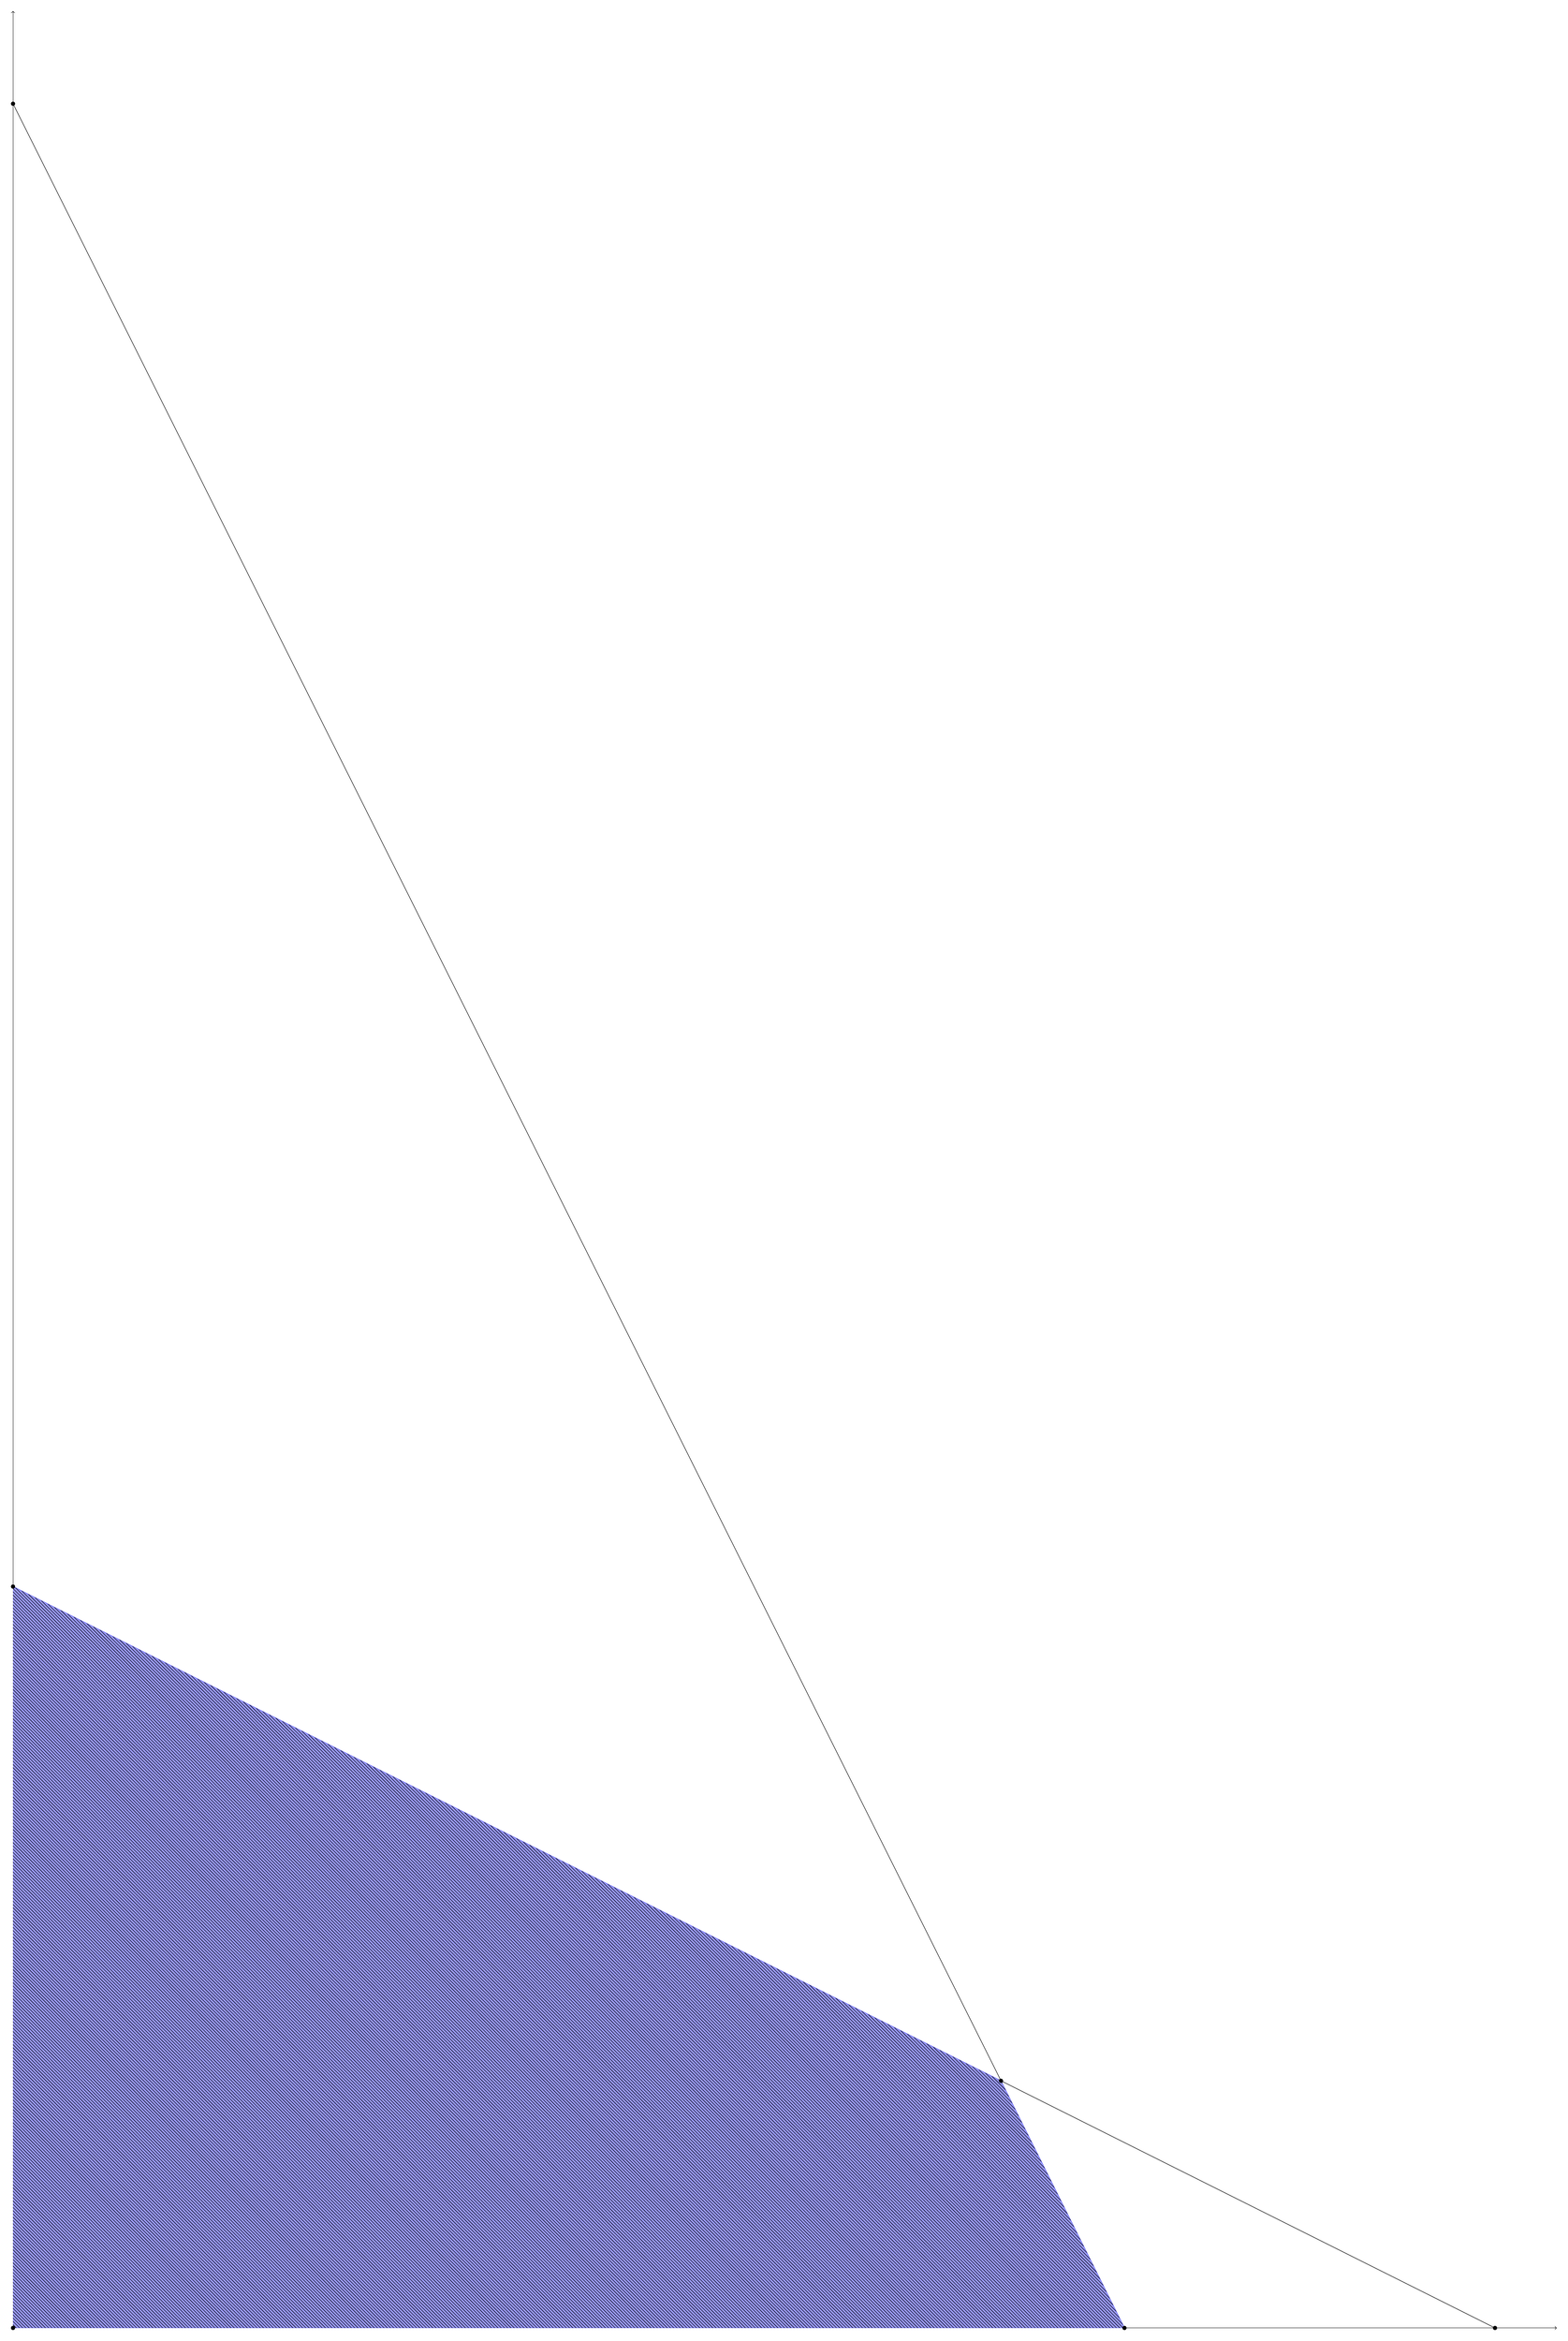
\begin{tikzpicture}
\coordinate (o) at (0,0);
\coordinate (a) at (36,0);
\coordinate (b) at (48,0);
\coordinate (c) at (32,8);
\coordinate (d) at (0,24);
\coordinate (e) at (0,72);
\draw[->] (o) -- (50,0);
\draw[->] (o) -- (0,75);
\draw[-,blue] (a) -- (o);
\draw[-,blue] (a) -- (c);
\draw[-,blue] (d) -- (c);
\draw[-,blue] (d) -- (o);
\fill [blue!40!white] (o) -- (a) -- (c) -- (d) -- (o);
\pattern [pattern=north west lines] (o) -- (a) -- (c) -- (d) -- (o);
\draw[-] (b) -- (c);
\draw[-] (e) -- (c);
\foreach \x in {a,b,c,d,e,o}
{
\fill (\x) circle (2pt);
}

\end{tikzpicture}
}
  \end{figure}
\subsection{}

Maximize 
\begin{align*}
Z           & = 117 x_1 + 111 x_2 \\
\end{align*}
subject to
\begin{align*}
9 x_1+5 x_2 & \ge 50              \\
7 x_1+9 x_2 & \ge 30              \\
5 x_1+3 x_2 & \le 150             \\
7 x_1+9 x_2 & \le 190             \\
2 x_1+4 x_2 & \le 100             \\
x_1         & \ge 0               \\
x_2         & \ge 0
\end{align*}

  \begin{figure}[H]
    \centering
\scalebox{0.25}{
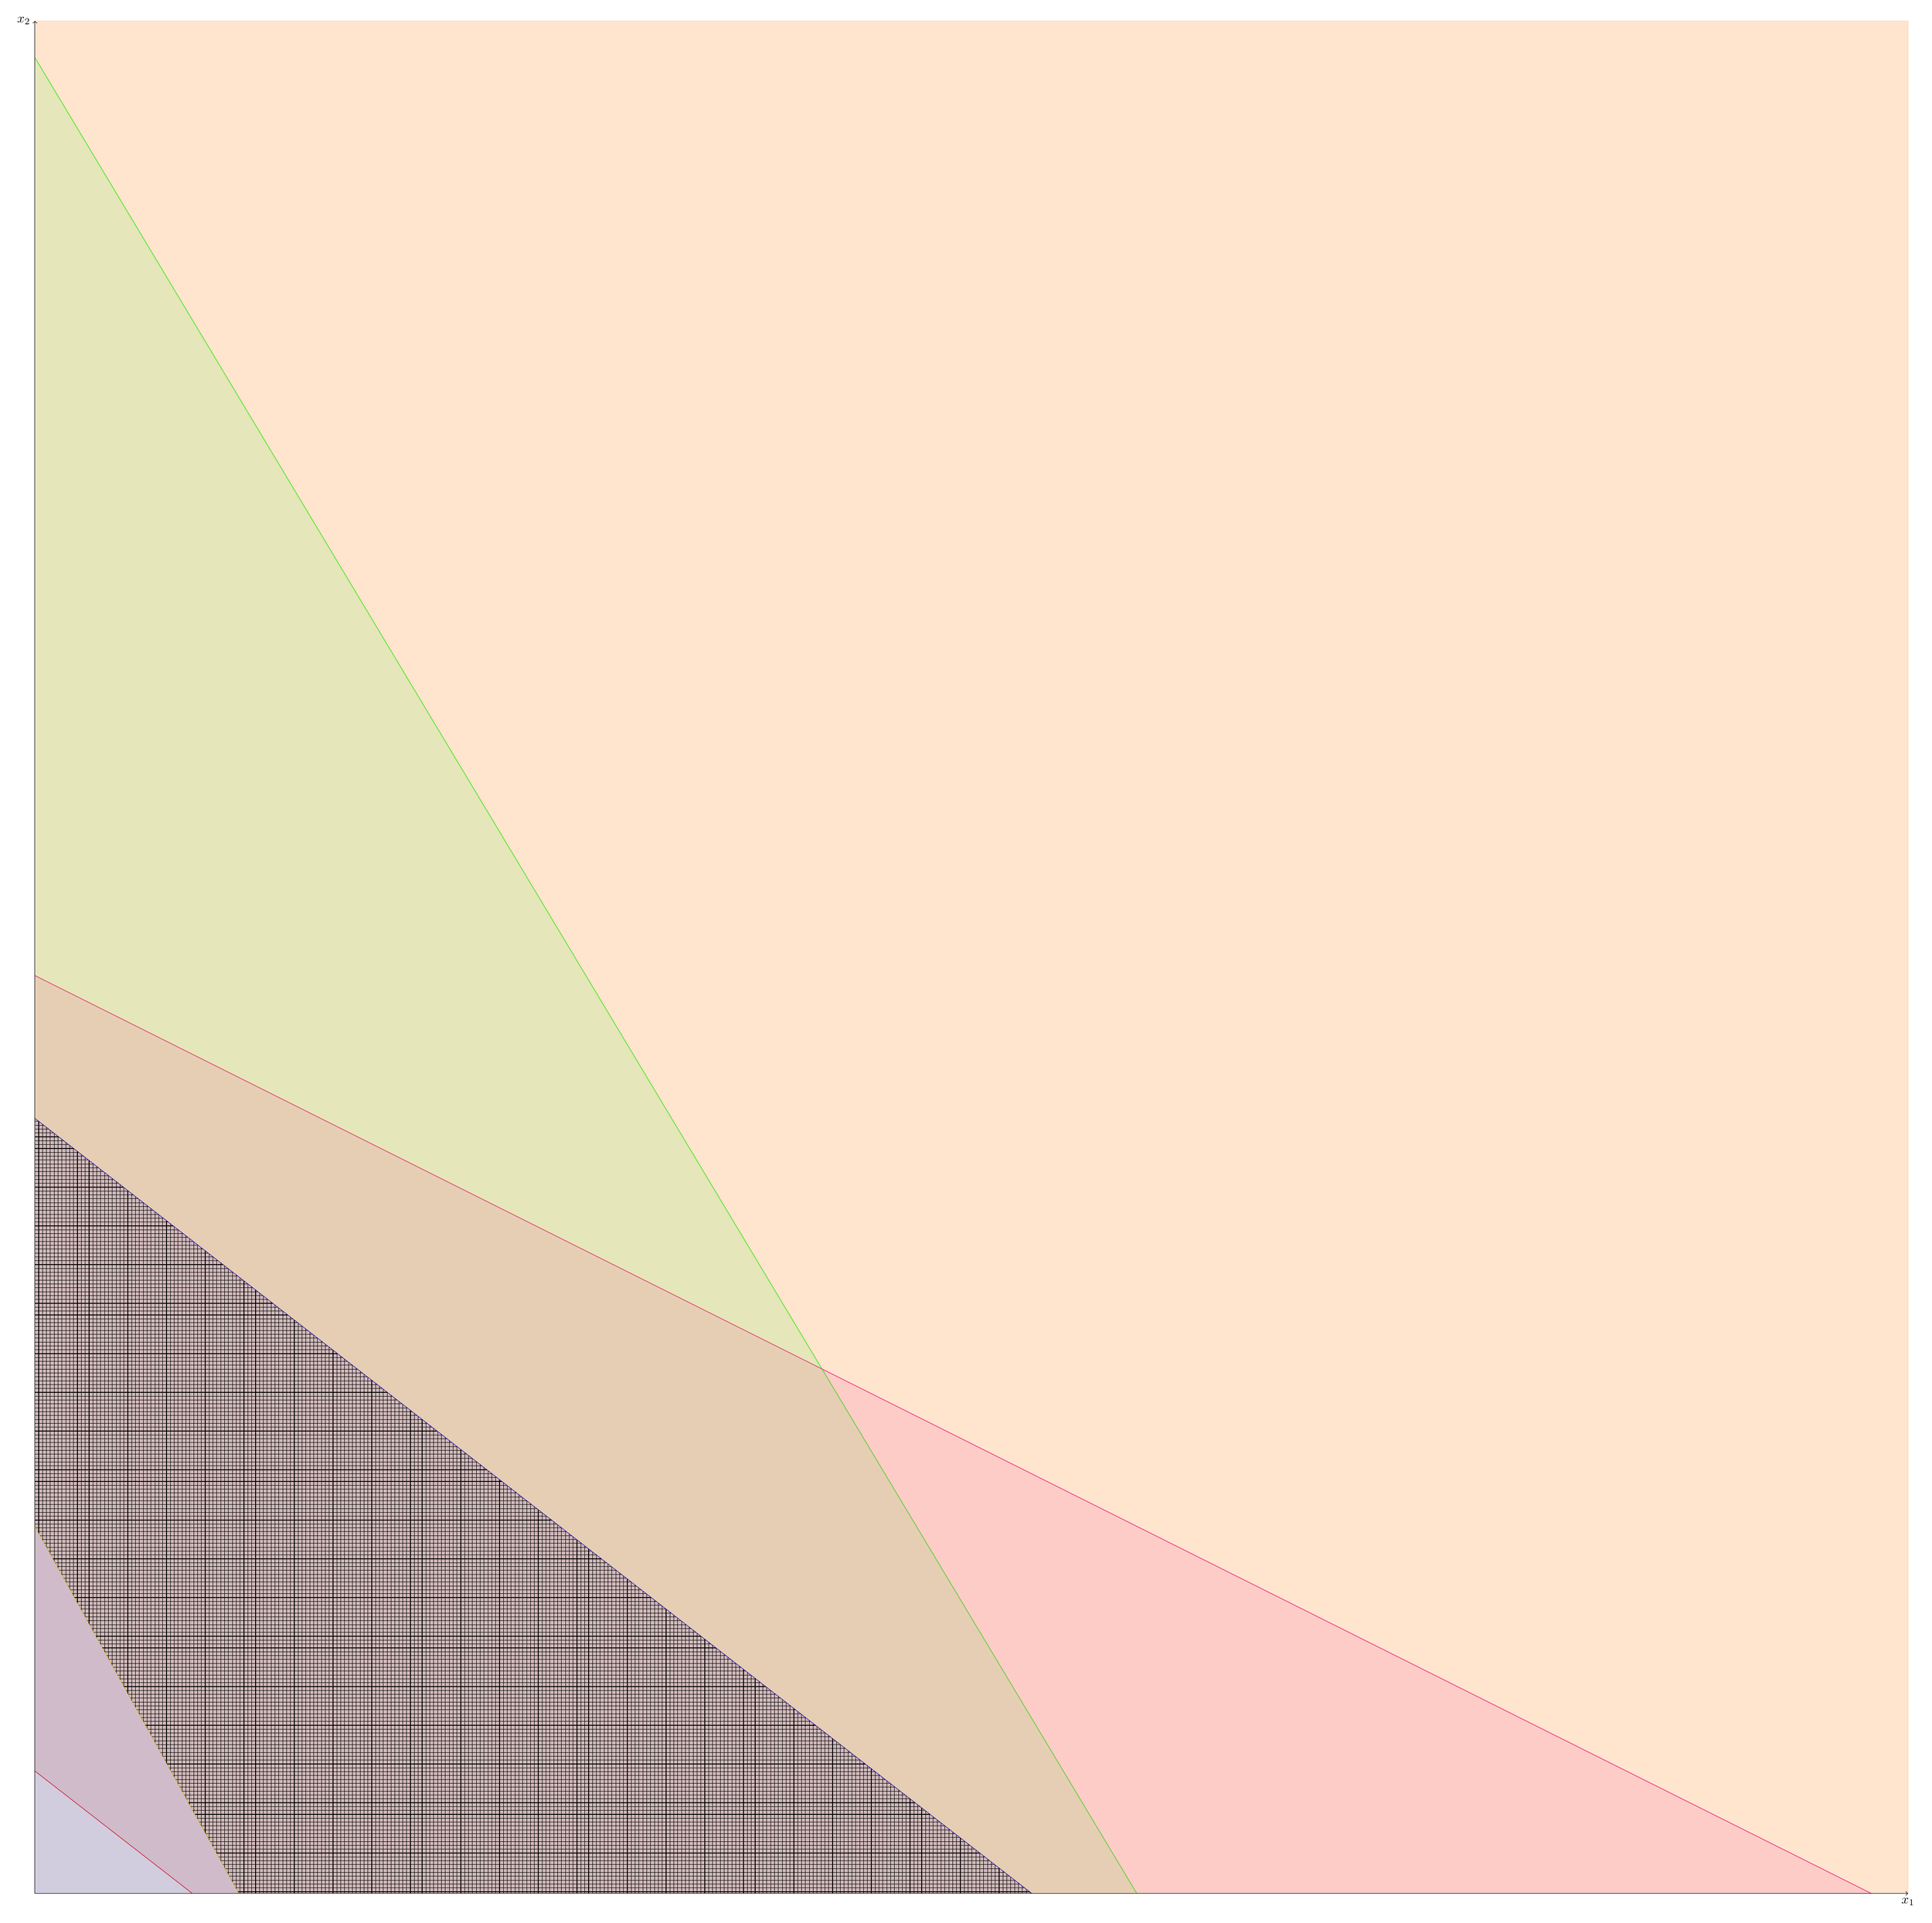
\begin{tikzpicture}
\coordinate (o) at (0,0);
\coordinate (a) at (50/9,0);
\coordinate (b) at (190/7,0);
\coordinate (c) at (0,190/9);
\coordinate (d) at (0,10);
\coordinate (f) at (190/7,190/9);
\coordinate (tl) at (0,51);
\coordinate (tr) at (51,51);
\coordinate (br) at (51,0);

 \draw[-, color=yellow]  (0,10) -- (50/9,0) ;
 \draw[-, color=red]  (0,10/3) -- (30/7,0) ;
 \draw[-, color=green]  (0,50) -- (30,0) ;
 \draw[-, color=blue]  (c) -- (b);
 \draw[-, color=magenta]  (0,25) -- (50,0) ;
 \filldraw[color=yellow,  opacity=0.1]  (0,10) -- (50/9,0) -- (br) -- (tr) -- (tl) -- (0,10) -- cycle;
 \filldraw[color=red,  opacity=0.1]  (0,10/3) -- (30/7,0) -- (br) -- (tr) -- (tl) --(0,10/3) -- cycle;
 \filldraw[color=green,  opacity=0.1]  (0,50) -- (30,0) -- (o) -- (0,50)  -- cycle;
 \filldraw[color=blue,  opacity=0.1]  (b) -- (o) -- (c) -- (b) -- cycle;
 \filldraw[color=magenta,  opacity=0.1]  (0,25) -- (50,0) -- (o) -- (0,25)  -- cycle;
 \pattern [pattern=grid]  (a) -- (b) -- (c) -- (d) -- (a);
 \draw[->] (o) -- (br)node[below]{$x_1$} ;
 \draw[->] (o) -- (tl)node[left]{$x_2$} ;
\end{tikzpicture}
}
\end{figure}
Optimal solution is $\left(\frac{190}{7}, 0\right)$, and Max $Z=\frac{22230}{7}\approx 3175.71429$

\subsection{}

Maximize the value of
\begin{align*}
Z           & = 60 x_1 + 60 x_2 \\
\end{align*}
Subject to 
\begin{align*}
x_1+x_2     & \le 12            \\
2 x_1+3 x_2 & \ge 60            \\
 x_1        & \ge 0             \\
 x_2        & \ge 0  
\end{align*}

  \begin{figure}[H]
    \centering
\scalebox{0.5}{
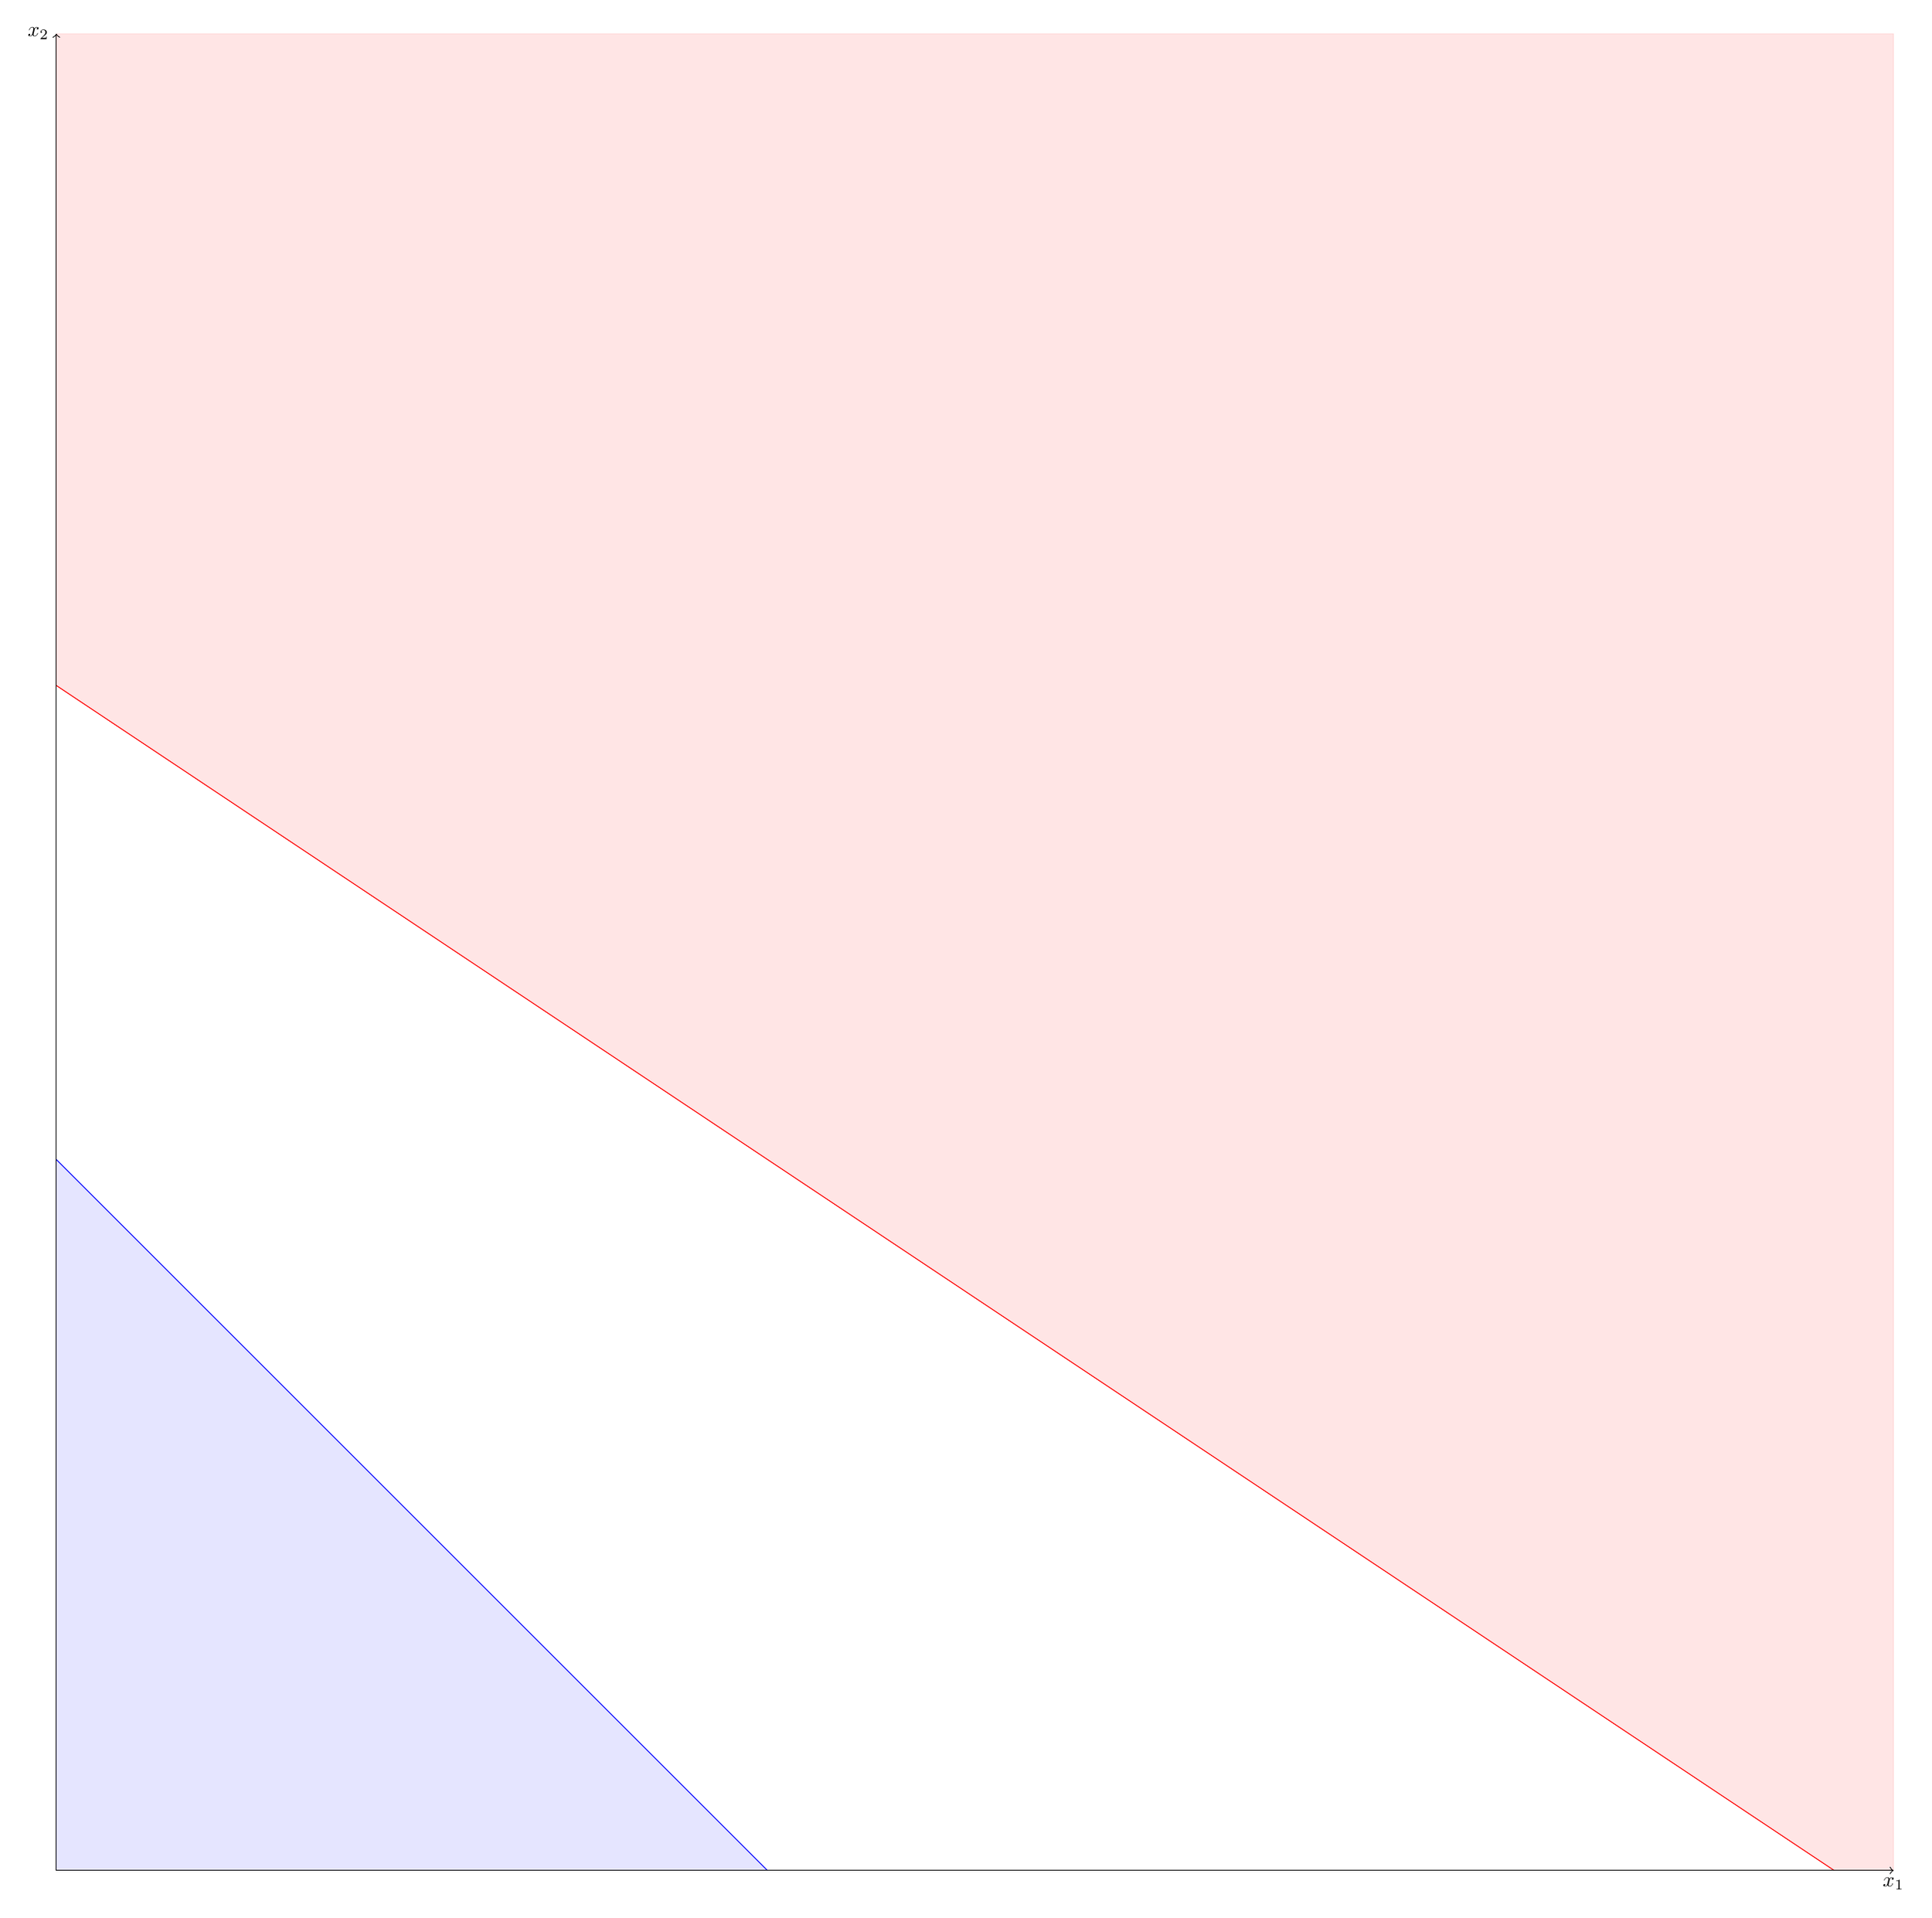
\begin{tikzpicture}
\coordinate (tl) at (0,31);
\coordinate (tr) at (31,31);
\coordinate (br) at (31,0);
\coordinate (o) at (0,0);
 \draw[-, color=blue]  (0,12) -- (12,0);
 \draw[-, color=red]  (0,20) -- (30,0);
 \filldraw[color=blue,  opacity=0.1] (0,12) -- (12,0) -- (o) -- (0,12) -- cycle;
 \filldraw[color=red,  opacity=0.1]  (0,20) -- (30,0) -- (br) -- (tr) -- (tl) --(0,20) -- cycle;
 \draw[->] (o) -- (br)node[below]{$x_1$} ;
 \draw[->] (o) -- (tl)node[left]{$x_2$} ;
\end{tikzpicture}
}
\end{figure}
There is no feasible region, hence no feasible solution too.

\subsection{}

Maximize 
\begin{align*}
Z       & = 2 x_1+3 x_2 \\
\end{align*}
subject to 
\begin{align*}
x_1-x_2 & \le 2         \\
x_1+x_2 & \ge 4         \\
x_1,x_2 & \ge 0
\end{align*}
  \begin{figure}[H]
    \centering
\scalebox{0.5}{
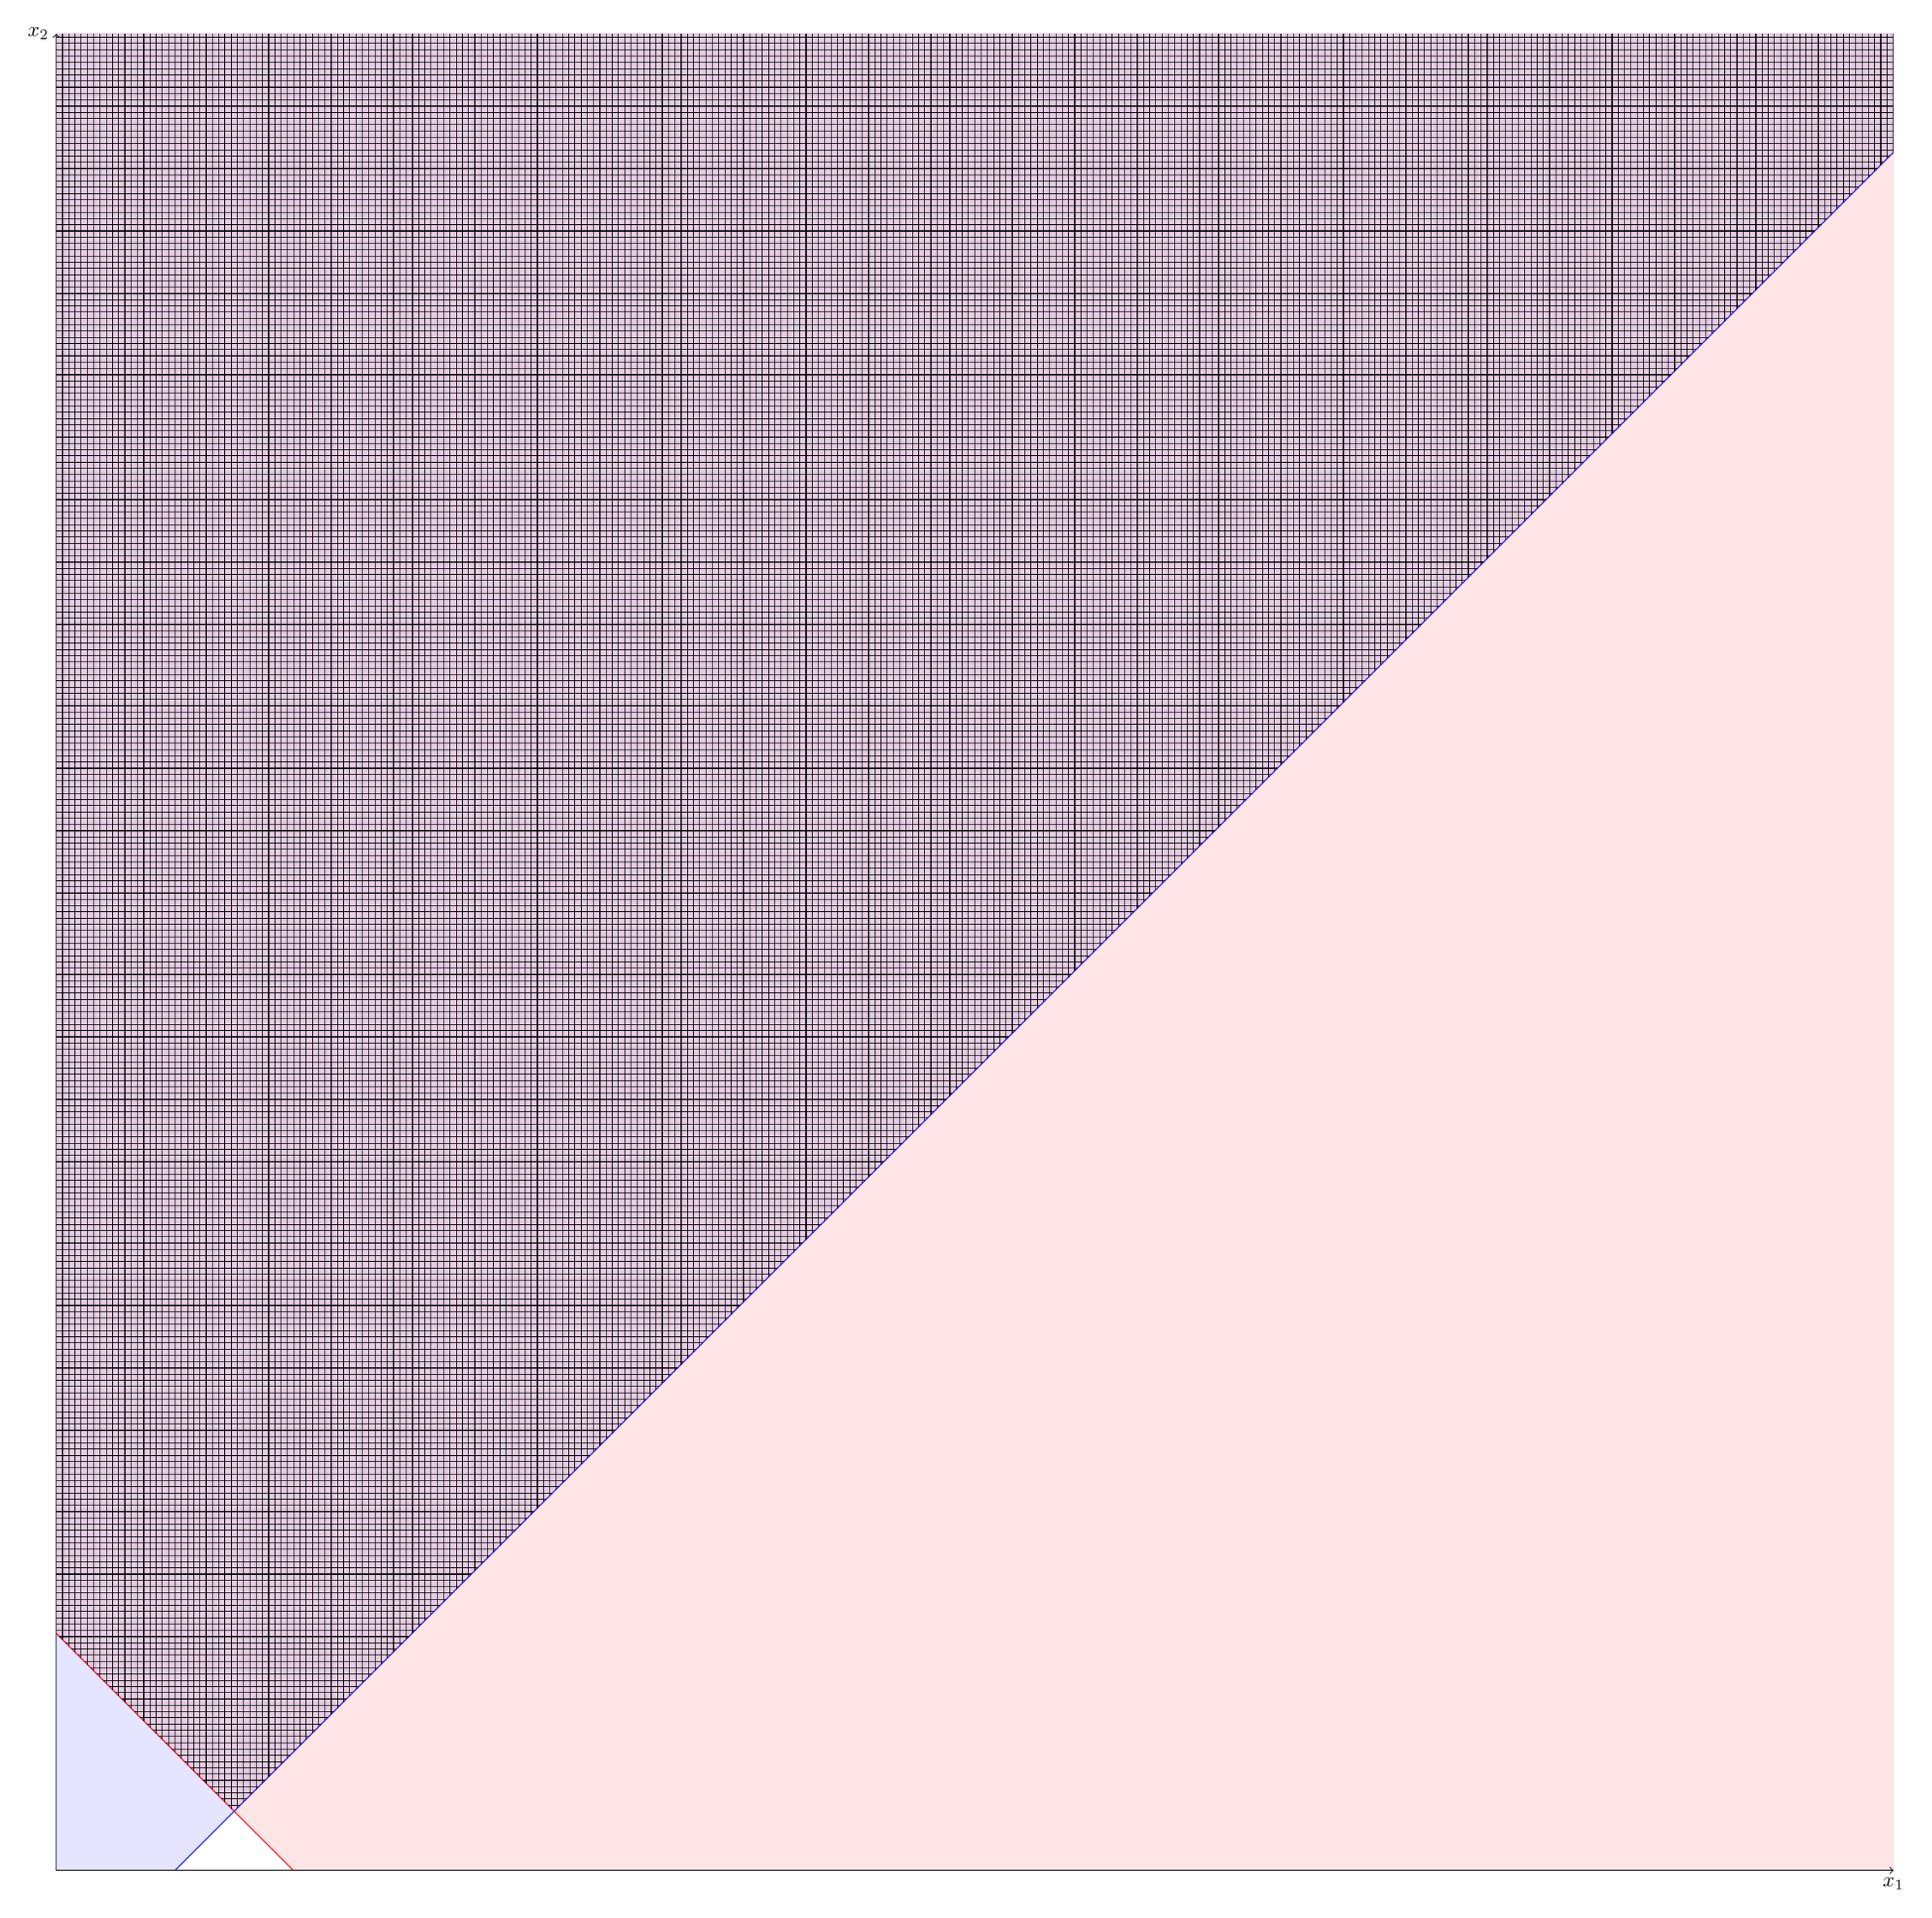
\begin{tikzpicture}
\coordinate (tl) at (0,31);
\coordinate (tr) at (31,31);
\coordinate (br) at (31,0);
\coordinate (o) at (0,0);
 \draw[-, color=blue]  (2,0) -- (31,29);
 \draw[-, color=red]  (0,4) -- (4,0);
 \filldraw[color=blue,  opacity=0.1]  (2,0) -- (31,29) -- (tr) -- (tl) -- (o) -- (2,0) -- cycle;
 \filldraw[color=red,  opacity=0.1]  (0,4) -- (4,0) -- (br) -- (tr) -- (tl) --(0,4) -- cycle;
 \pattern [pattern=grid]  (0,4) -- (3,1) -- (31,29) -- (tr) -- (tl) -- (0,4);
 \draw[->] (o) -- (br)node[below]{$x_1$} ;
 \draw[->] (o) -- (tl)node[left]{$x_2$} ;
\end{tikzpicture}
}
\end{figure}

The feasible region is unbounded, which means the max value occurs at infinity.

It can be called as an unbounded feasible solution.
\subsection{}

Maximize 
\begin{align*}
Z            & = 15 x_1 + 9 x_2 \\
\end{align*}
Subject to 
\begin{align*}
10 x_1+6 x_2 & \le 60           \\
x_1+2 x_2    & \le 10           \\
x_1          & \ge 0            \\
x_2          & \ge 0            \\
\end{align*}

  \begin{figure}[H]
    \centering
\scalebox{1}{
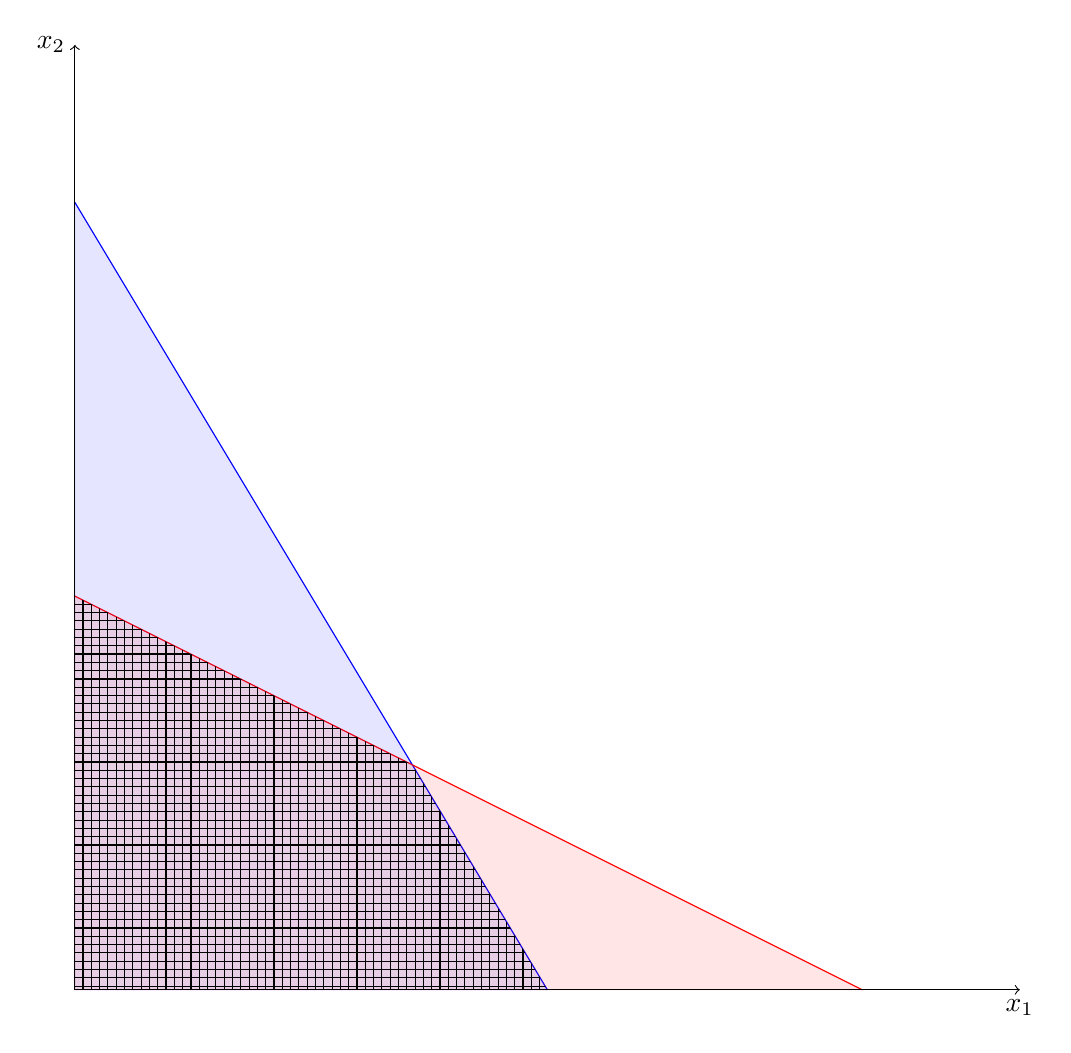
\begin{tikzpicture}
\coordinate (tl) at (0,12);
\coordinate (tr) at (12,12);
\coordinate (br) at (12,0);
\coordinate (o) at (0,0);
 \draw[-, color=blue]  (0,10) -- (6,0);
 \draw[-, color=red]  (0,5) -- (10,0);
 \filldraw[color=blue,  opacity=0.1]  (0,10) -- (6,0) -- (o) -- (0,10);
 \filldraw[color=red,  opacity=0.1]  (0,5) -- (10,0) -- (o) -- (0,5);
 \pattern [pattern=grid]  (0,5) -- (30/7,20/7) -- (6,0) -- (o) -- (0,10);
 \draw[->] (o) -- (br)node[below]{$x_1$} ;
 \draw[->] (o) -- (tl)node[left]{$x_2$} ;
\end{tikzpicture}
}
\end{figure}

The objective function is parallel to the constraint $10x_1+6x_2\le 60$, and the Max $Z=90$ for the corner feasible points 
$\left(\frac{30}{7}, \frac{20}{7}\right)$ and $\left(6,0\right)$, which lie on the mentioned constraint. Hence, there are multiple optimal 
solutions on that line. 

\subsection{}

Maximize 
\begin{align*}
Z           & = x_1 - 2 x_2 \\
\end{align*}
Subject to 
\begin{align*}
-x_1+x_2    & \le 1         \\
6 x_1+4 x_2 & \ge 24        \\
0 \le x_1   & \le 5         \\
2 \le x_2   & \le 4         \\
\end{align*}

  \begin{figure}[H]
    \centering
\scalebox{1}{
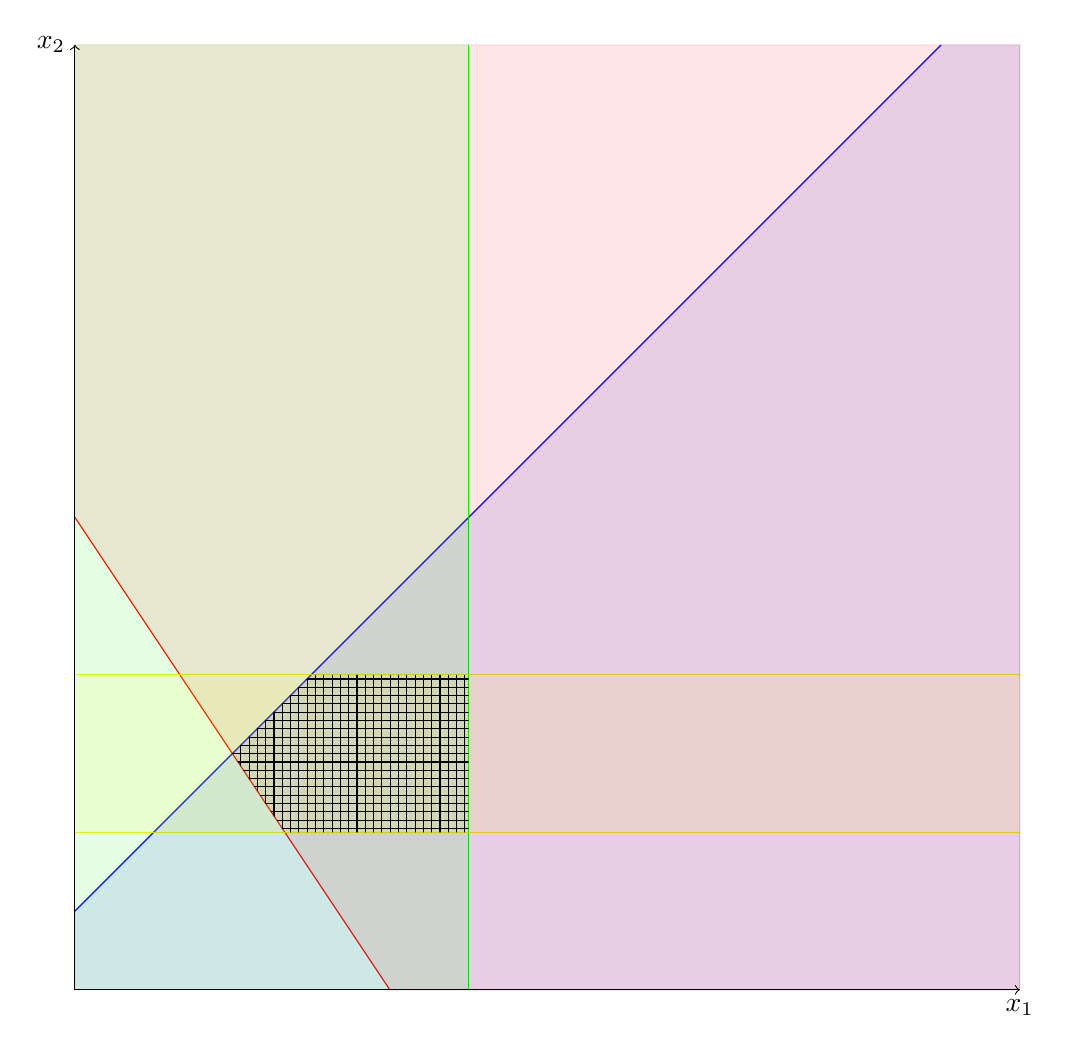
\begin{tikzpicture}
\coordinate (tl) at (0,12);
\coordinate (tr) at (12,12);
\coordinate (br) at (12,0);
\coordinate (o) at (0,0);
 \draw[-, color=blue]  (0,1) -- (11,12);
 \draw[-, color=red]  (0,6) -- (4,0);
 \draw[-, color=green]  (5,0) -- (5,12);
 \draw[-, color=yellow]  (0,4) -- (12,4);
 \draw[-, color=yellow]  (0,2) -- (12,2);
 \filldraw[color=blue,  opacity=0.1] (0,1) -- (11,12) -- (tr) -- (br) -- (o) -- (0,1);
 \filldraw[color=red,  opacity=0.1] (0,6) -- (4,0) -- (br) -- (tr) -- (tl) -- (0,6);
 \filldraw[color=green,  opacity=0.1] (5,0) -- (5,12) -- (tl) -- (o) -- (5,0);
 \filldraw[color=yellow,  opacity=0.1] (0,4) -- (0,2) -- (12,2) -- (12,4) -- (0,4);
 \pattern [pattern=grid]  (2,3) -- (3,4) -- (5,4) -- (5,2) -- (8/3,2) -- (2,3);
 \draw[->] (o) -- (br)node[below]{$x_1$} ;
 \draw[->] (o) -- (tl)node[left]{$x_2$} ;
\end{tikzpicture}
}
\end{figure}

Max $Z=1$ at $\left(5,2\right)$

\subsection{}

Minimize 
\begin{align*}
Z              & = 3 x_1+5 x_2 \\
\end{align*}
Subject to 
\begin{align*}
-3 x_1 + 4 x_2 & \le 12        \\
2 x_1 - x_2    & \ge -2        \\
2 x_1 + 3 x_2  & \ge 12        \\
 x_1           & \le 4         \\
 x_2           & \ge 2         \\
 x_1           & \ge 0         \\
\end{align*}

 \begin{figure}[H]
    \centering
\scalebox{1}{
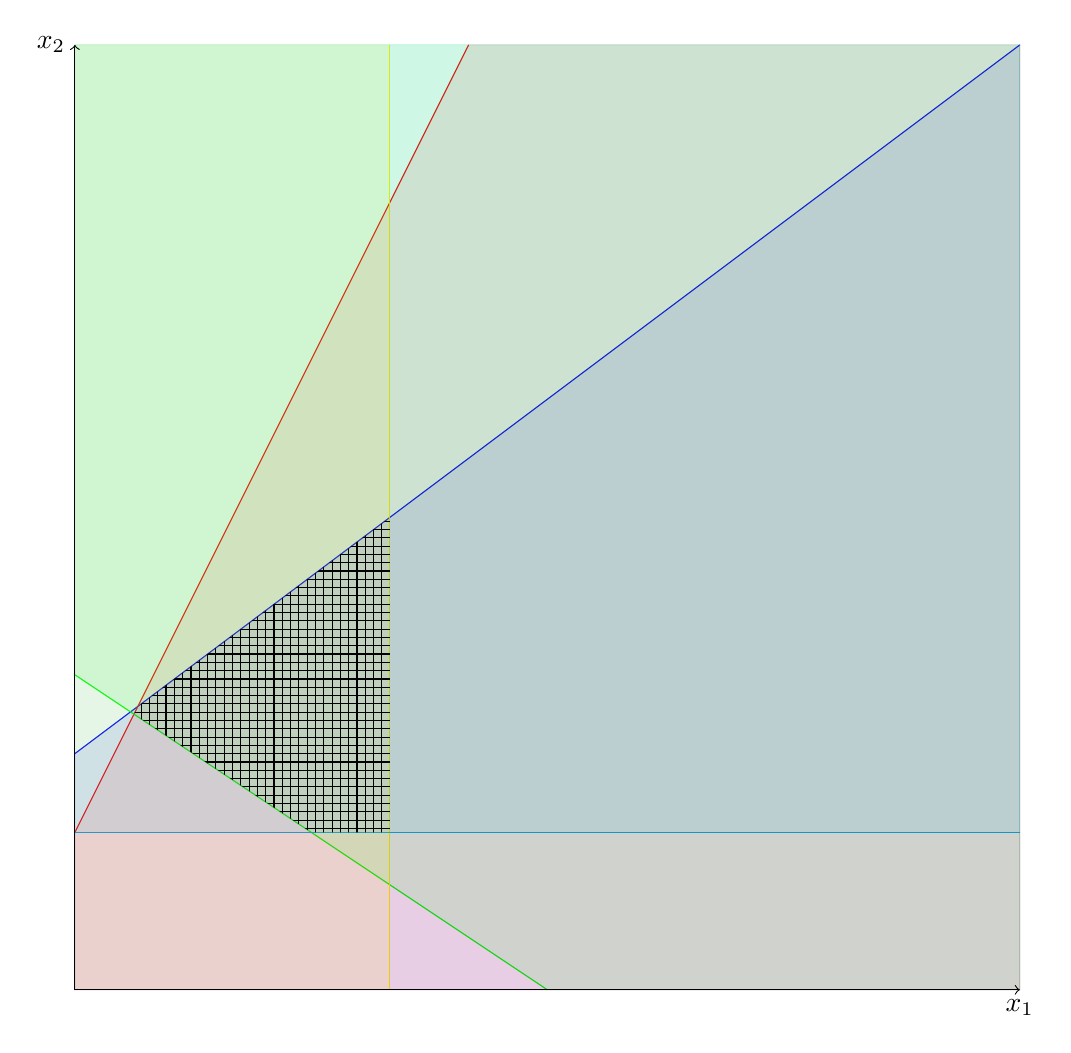
\begin{tikzpicture}
\coordinate (tl) at (0,12);
\coordinate (tr) at (12,12);
\coordinate (br) at (12,0);
\coordinate (o) at (0,0);
 \draw[-, color=blue]  (0,3) -- (12,12);
 \draw[-, color=red]  (0,2) -- (5,12);
 \draw[-, color=green]  (0,4) -- (6,0);
 \draw[-, color=yellow]   (4,0) -- (4,12);
 \draw[-, color=cyan]  (0,2) -- (12,2);
 \filldraw[color=blue,  opacity=0.1] (0,3) -- (12,12) -- (br) -- (o) -- (0,3);
 \filldraw[color=red,  opacity=0.1] (0,2) -- (5,12) -- (tr) -- (br) -- (o) -- (0,2);
 \filldraw[color=green,  opacity=0.1] (0,4) -- (6,0) -- (br) -- (tr) -- (tl) -- (0,2);
 \filldraw[color=yellow,  opacity=0.1] (4,0) -- (4,12) --  (tl) -- (o) -- (4,0);
 \filldraw[color=cyan,  opacity=0.1] (0,2) -- (12,2) -- (tr) -- (tl) -- (0,2);
 \pattern [pattern=grid]  (4/5,18/5) -- (3/4,7/2) -- (3,2) -- (4,2) -- (4,6) -- (4/5,18/5);
 \draw[->] (o) -- (br)node[below]{$x_1$} ;
 \draw[->] (o) -- (tl)node[left]{$x_2$} ;
\end{tikzpicture}
}
\end{figure}
Min $Z=19$ at $\left(3,2\right)$

\subsection{}

Maximize 
\begin{align*}
Z            & = 3 x_1 + 2 x_2 \\
\end{align*}
Subject to 
\begin{align*}
x_1 + 3 x_2  & \le 15          \\
2 x_1 +  x_2 & \le 10          \\
0 \le x_1    & \le 4           \\
x_2          & \ge 0
\end{align*}

Also, 
\begin{enumerate}
\item Identify the feasible and infeasible regions
\item Write all the CPF solutions and CP infeasible solutions
\end{enumerate}

\begin{figure}[H]
    \centering
\scalebox{1}{
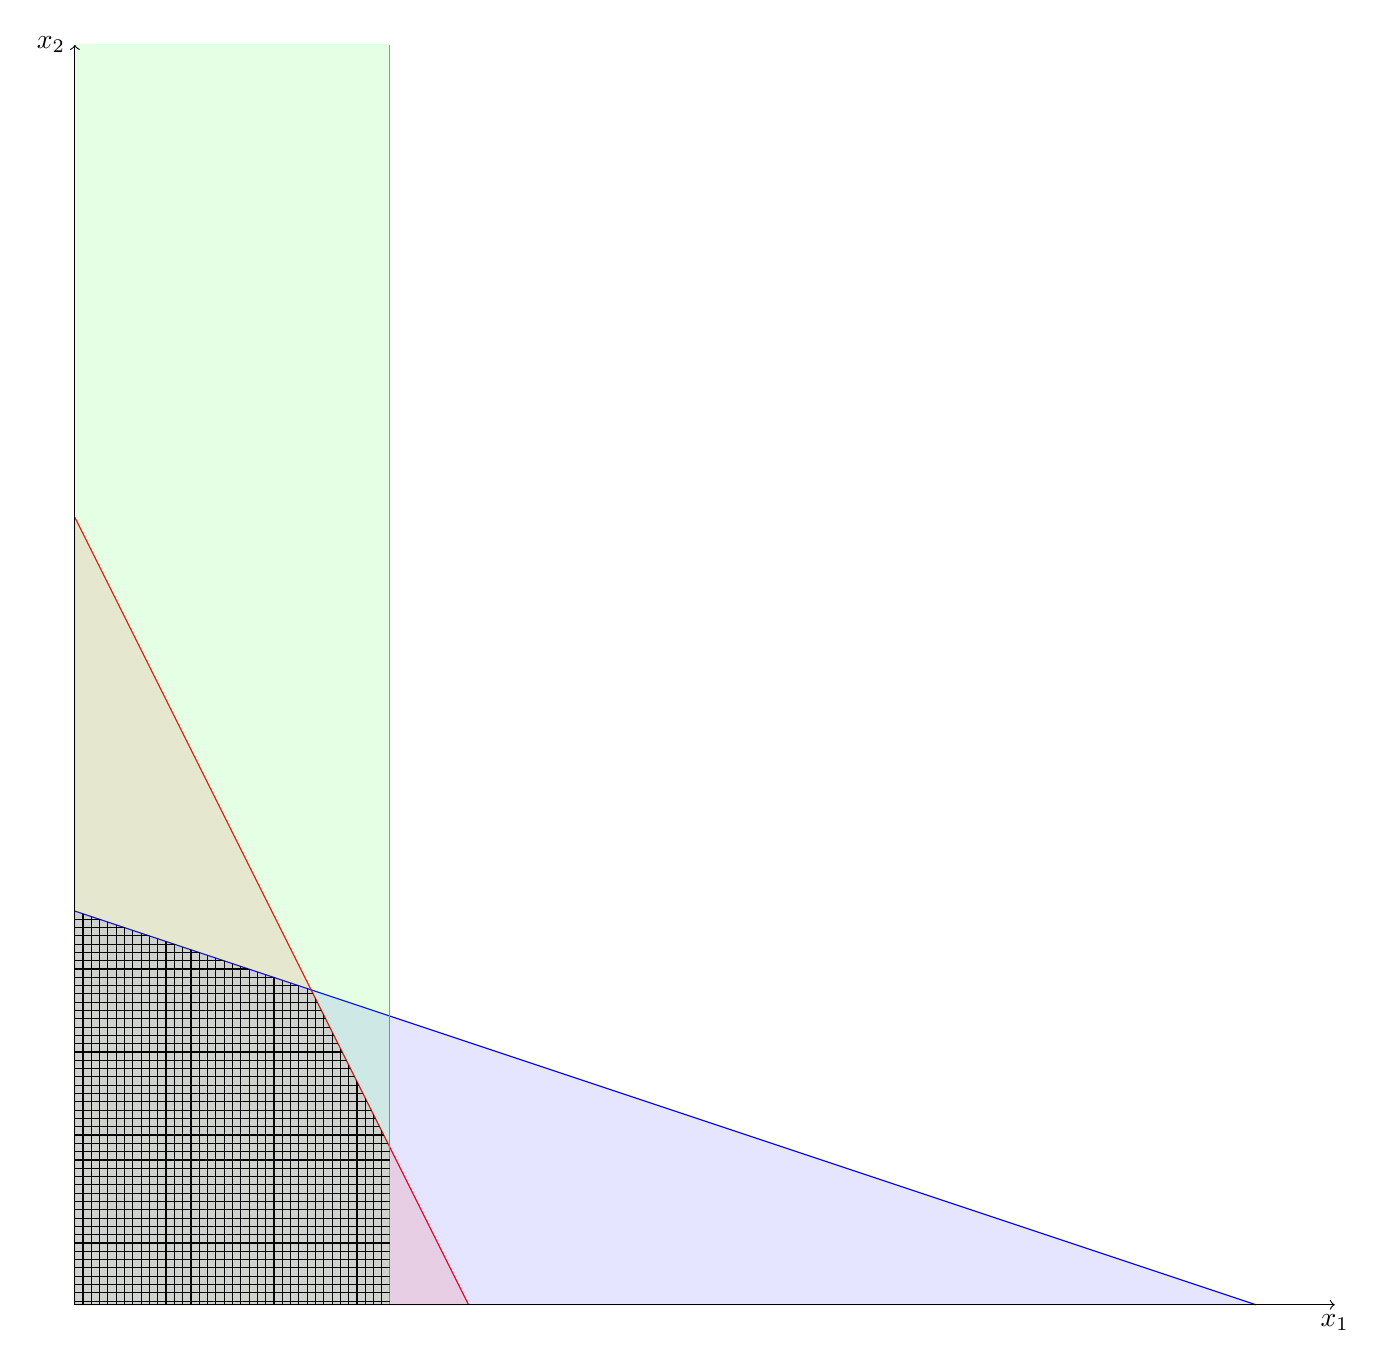
\begin{tikzpicture}
\coordinate (tl) at (0,16);
\coordinate (tr) at (16,16);
\coordinate (br) at (16,0);
\coordinate (o) at (0,0);
 \draw[-, color=blue]  (0,5) -- (15,0);
 \draw[-, color=red]  (0,10) -- (5,0);
 \draw[-, color=green]  (4,0) -- (4,16);
 \filldraw[color=blue,  opacity=0.1] (0,5) -- (15,0) -- (o) -- (0,5);
 \filldraw[color=red,  opacity=0.1] (0,10) -- (5,0) -- (o) -- (0,10);
 \filldraw[color=green,  opacity=0.1] (4,0) -- (4,16) -- (tl) -- (o) -- (4,0);
 \pattern[pattern=grid] (0,5) -- (3,4) -- (4,2) -- (4,0) -- (o) -- (0,5);
 \draw[->] (o) -- (br)node[below]{$x_1$} ;
 \draw[->] (o) -- (tl)node[left]{$x_2$} ;
\end{tikzpicture}
}
\end{figure}

The gridded area is the feasible region, and the area outside it is the infeasible region.

The points lying on the gridded area are the corner point feasible solutions, and the remaining points are the 
corner point infeasible solutions. 

\section{Simplex Method}
\subsection{}


\subsubsection*{The essence of simplex method}
\begin{itemize}
\item Five constraint boundaries and their points of intersection
\item Points of intersection are \textbf{corner point solutions}
\item Those on the corners of the feasible region are called \textbf{CPF solutions}
\item Each corner point solution lies in the intersection of two constraint boundaries
\item For a LPP with n decision variables, two CPF solutions are adjacent if they share $n-1$ constraint boundaries
\item The line segment connecting the two adjacent points is called edge of the feasible region
\item Optimality test: Any LPP that possesses at least one optimal solution, if a CPF solution has no adjacnet CPF solutions 
that are better, then it must be an optimal solution
\end{itemize}

  \subsubsection*{The essence}
Consider the following LPP and its associated graph:

Maximize $Z=3 x_1 + 5 x_2$

Subject to 
\begin{align*}
x_1           & \le 4  \\
2 x_2         & \le 12 \\
3 x_1 + 2 x_2 & \le 18 \\
\end{align*}
and 
$x_1 \ge 0, x_2 \ge 0$

  \begin{figure}[h]
    \centering
\scalebox{0.5}{      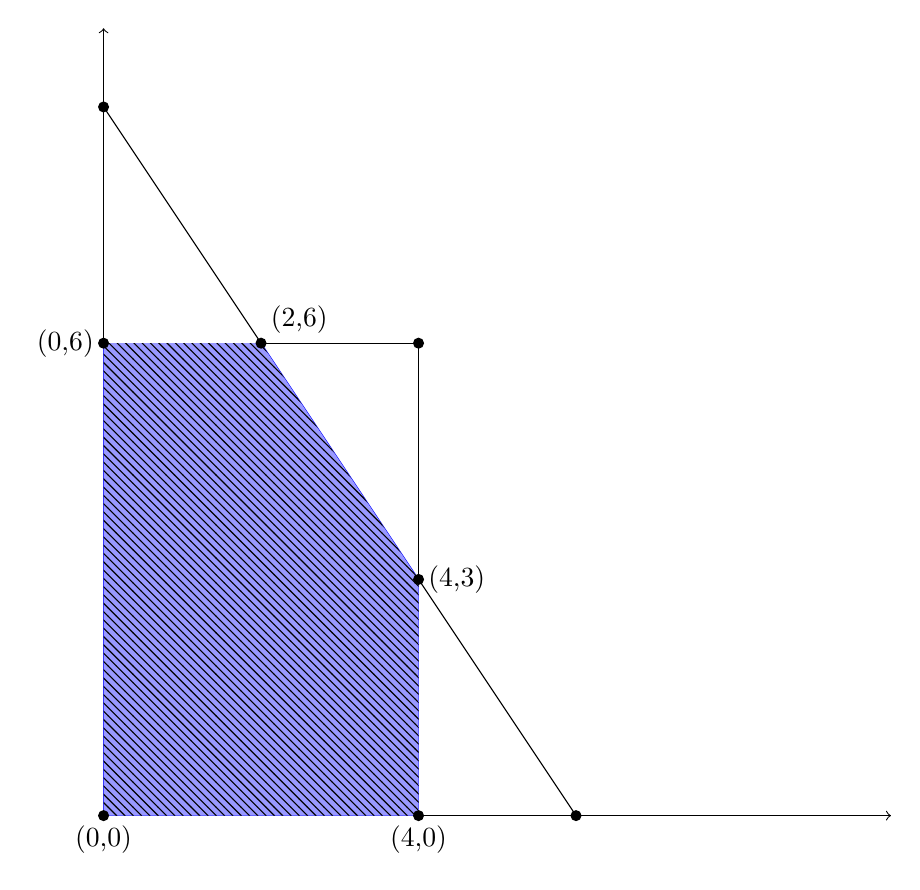
\begin{tikzpicture}
\coordinate (o) at (0,0);
\coordinate (a) at (4,0);
\coordinate (b) at (6,0);
\coordinate (c) at (4,3);
\coordinate (d) at (4,6);
\coordinate (e) at (2,6);
\coordinate (f) at (0,6);
\coordinate (g) at (0,9);
\draw[->] (o) -- (10,0);
\draw[->] (o) -- (0,10);
\draw[-,blue] (a) -- (o);
\draw[-,blue] (a) -- (c);
\draw[-,blue] (e) -- (c);
\draw[-,blue] (f) -- (e);
\draw[-,blue] (f) -- (o);
\fill [blue!40!white] (o) -- (a) -- (c) -- (e) -- (f) -- (o);
\pattern [pattern=north west lines] (o) -- (a) -- (c) -- (e) -- (f) -- (o);
\draw[-] (b) -- (c);
\draw[-] (d) -- (c);
\draw[-] (d) -- (e);
\draw[-] (g) -- (e);
\draw (o) node[below] {(0,0)};
\draw (a) node[below] {(4,0)};
\draw (c) node[right] {(4,3)};
\draw (e) node[above right] {(2,6)};
\draw (f) node[left] {(0,6)};
\foreach \x in {a,b,c,d,e,f,g,o}
{
\fill (\x) circle (2pt);
}

\end{tikzpicture}
}
    \caption{Constraint boundaries and CPF}
  \end{figure}


  \begin{itemize}
  \item Initialization: Choose (0, 0) as the initial CPF solution to examine. 
  \item Optimality Test: Conclude that (0, 0) is not an optimal solution. 
  \item Iteration 1: Move to a better adjacent CPF solution, (0, 6), by performing the following three steps:
    \begin{enumerate}
    \item Considering the two edges of the feasible region that emanate from (0, 0), choose to move
along the edge that leads up the $x_2$ axis. ($x_2$ axis increases Z at a faster rate than moving along the $x_1$ axis)
\item Stop at the first new constraint boundary: $2x_2 = 12$. 
\item Solve for the intersection of the new set of constraint boundaries: (0, 6). 
    \end{enumerate}
\item Continue with optimality test and iteration 2, and conclude the optimal solution
  \end{itemize}



\subsubsection*{The key solution concepts}
\begin{itemize}
\item The simplex method focuses solely on CPF solutions. For
any problem with at least one optimal solution, finding one requires only finding a best CPF solution
\item The simplex method is an iterative algorithm (a systematic
solution procedure that keeps repeating a fixed series of steps, called an iteration,
until a desired result has been obtained) 
\item Whenever possible, the initialization of the simplex method
chooses the origin (all decision variables equal to zero) to be the initial CPF solution. 
\item Given a CPF solution, it is much quicker computationally
to gather information about its adjacent CPF solutions than about other CPF solutions. 
the entire path followed to eventually reach an optimal solution is along
the edges of the feasible region.
\end{itemize}



\begin{itemize}
\item After the current CPF solution is identified, the simplex
method examines each of the edges of the feasible region that emanate from this
CPF solution. 
It simply identifies the rate of improvement in Z that would
be obtained by moving along the edge. Among the edges with a positive rate of
improvement in Z, it then chooses to move along the one with the largest rate of
improvement in Z
\item The optimality test consists simply of checking whether
any of the edges give a positive rate of improvement in Z. If none do, then the
current CPF solution is optimal
\end{itemize}




\subsubsection*{Setting up the simplex method}
\begin{itemize}
\item It's an algebraic procedure -- first step is to convert the inequalities to equivalent equality constraints
\item Introduce slack variables

E.g. $x_1 \le 4$, slack variable is $x_3 = 4 - x_1 $
\end{itemize}

Maximize $$Z=3 x_1 + 5 x_2$$

Subject to 
\begin{align*}
x_1           & \le 4  \\
2 x_2         & \le 12 \\
3 x_1 + 2 x_2 & \le 18 \\
\end{align*}
and 
$x_1 \ge 0, x_2 \ge 0$

In the simplex method, the LPP is converted to its standard form by adding slack variables to the constraints:

Maximize $$Z=3 x_1 + 5 x_2$$

Subject to 
\begin{align*}
x_1 +x_3& = 4   \\
2 x_2 +x_4& = 12 \\
3 x_1 + 2 x_2+x_5 & = 18 \\
\end{align*}
and 
$x_i \ge 0$ for $i=1,2,3,4,5$

\begin{tabular}{r|l}
  slack variable & solution lies              \\ \hline
  = 0            & on the constraint boundary \\
  $>0$           & on the feasible side       \\ 
  $<0$           & on the infeasible side
\end{tabular}



  \begin{itemize}
  \item An augmented solution is a solution for the original variables (the decision variables) that has been augmented by the corresponding values of the slack variables
  \item A basic solution is an augmented corner-point solution
  \item A basic feasible (BF) solution is an augmented CPF solution
  \item Two BF solutions are adjacent if all but one of their nonbasic variables are the same.
This implies that all but one of their basic variables also are the same, although perhaps
with different numerical values
  \end{itemize}


  \begin{itemize}
\item Number of variables -- Number of equations $= 5-3=2$ degrees of freedom
\item 2 variables can be set to arbitrary values and solve the system of equations (3 variables, 3 equations)
  \item 2 variables are called nonbasic variables (set to zero)
  \item The simultaneous solution of the other three variables (basic variables) is called basic solution
  \end{itemize}


  \subsubsection*{Properties of basic solution}
  \begin{enumerate}
  \item Each variable is designated as either a nonbasic variable or a basic variable.
  \item The number of basic variables equals the number of functional constraints (now equations). Therefore, the number of nonbasic 
variables equals the total number of variables minus the number of functional constraints.
\item The nonbasic variables are set equal to zero.
\item The values of the basic variables are obtained as the simultaneous solution of the system of equations (set of basic variables called as basis)
\item If the basic variables satisfy the nonnegativity constraints, the basic solution is a BF solution.
  \end{enumerate}
Two BF solutions are adjacent if all but one of their nonbasic variables are the same.
This implies that all but one of their basic variables also are the same, although perhaps
with different numerical values.


  \subsubsection*{The algebra of simplex method}
  \begin{itemize}
  \item Initialization: $x_1$ and $x_2$ are nonbasic variables for the initial BF solution
  \item Optimality test: $Z=3 x_1 + 5 x_2$, rates of improvements are positive, so not optimal
  \item Determining the direction of movement: $x_2$ is the entering basic variable:
At any iteration of the simplex method, the purpose of step 1 is to choose one nonbasic
variable to increase from zero (while the values of the basic variables are adjusted to continue satisfying the system of equations). Increasing this nonbasic variable from zero will
convert it to a basic variable for the next BF solution. Therefore, this variable is called
the entering basic variable for the current iteration (because it is entering the basis)
  \end{itemize}


  \subsubsection*{The algebra of simplex method}
  \begin{itemize}
  \item Determining where to stop: Keeping $x_1=0$ (nonbasic variable)the equations become
    \begin{align*}
      x_1 &= 0 \\
      x_3 &= 4 \\
      x_4 &= 12 - 2 x_1 \\
      x_5 &= 18 - 2 x_2 
    \end{align*}
  \item Because of non negativity constraint, $x_2 \le 6$
  \item These calculations are called minimum ratio test
  \item $x_4$ is the leaving basic variable
  \end{itemize}



  \begin{itemize}
  \item Solving for the new BF solution:
    \begin{align*}
      Z-3 x_1-5 x_2       & = 0  \\
      x_1+x_3             & = 4  \\
      2 x_2 + x_4         & = 12 \\
      3 x_1 + 2 x_2 + x_5 & = 18 
    \end{align*}
\item Solve by Gaussian elimination: $(x_1,x_2,x_3,x_4,x_5) = (0,6,4,0,6)$, $Z=30$
  \end{itemize}



  \begin{itemize}
  \item Optimality test of the new BF solution: 

    $Z = 30 + 3 x_1 - \frac{5}{2}x_4$

    Increasing $x_1$ would lead to a better adjacent BF solution
  \item Iteration 2: $x_5 = 6 - 3 x_1 \ge 0 \implies x_1 \le \frac{6}{3} = 2$ is the minimum ratio
  \item Hence, $x_5$ is the leaving basic variable
  \item Under the new system of equations, $Z=36-\frac{3}{2}x_4-x_5$, and cannot increase either $x_4$ or $x_5$, hence, $Z=36$ is optimal
  \end{itemize}



  \begin{tabular}{cc|c|c|ccccc|c} \hline 
    \multicolumn{2}{c|}{}  &           & \multicolumn{6}{|c|}{Coefficient of} &                                                                                                                          \\ 
    Iteration              & Basic var & Eq.                                  & Z & $x_1$                  & $x_2$                   & $x_3$ & $x_4$          & $x_5$          & Right                   \\ \hline 
                           & Z         & 0                                    & 1 & -3                     & -5                      & 0     & 0              & 0              & 0                       \\ \cline{6-6}
                         0 & $x_3$     & 1                                    & 0 & 1                      & \multicolumn{1}{|c|}{0} & 1     & 0              & 0              & 4                       \\ \cline{5-10}
                           & $x_4$     & 2                                    & 0 & 0                      & \multicolumn{1}{|c|}{2} & 0     & 1              & 0              & \multicolumn{1}{c|}{12} \\ \cline{5-10}
                           & $x_5$     & 3                                    & 0 & 3                      & \multicolumn{1}{|c|}{2} & 0     & 0              & 1              & 18                      \\ \thline 
                           & Z         & 0                                    & 1 & -3                     & 0                       & 0     & $\frac{5}{2}$  & 0              & 30                      \\ \cline{5-5}
                         1 & $x_3$     & 1                                    & 0 & \multicolumn{1}{c|}{1} & 0                       & 1     & 0              & 0              & 4                       \\ 
                           & $x_2$     & 2                                    & 0 & \multicolumn{1}{c|}{0} & 1                       & 0     & $\frac{1}{2}$  & 0              & 6                       \\ \cline{5-10}
                           & $x_5$     & 3                                    & 0 & \multicolumn{1}{c|}{3} & 0                       & 0     & -1             & 1              & \multicolumn{1}{c|}{6}  \\  \thline
                           & Z         & 0                                    & 1 & 0                      & 0                       & 0     & $\frac{3}{2}$  & 1              & 36                      \\
                         2 & $x_3$     & 1                                    & 0 & 0                      & 0                       & 1     & $\frac{1}{3}$  & $-\frac{1}{3}$ & 2                       \\
                           & $x_2$     & 2                                    & 0 & 0                      & 1                       & 0     & $\frac{1}{2}$  & 0              & 6                       \\
                           & $x_1$     & 3                                    & 0 & 1                      & 0                       & 0     & $-\frac{1}{3}$ & $\frac{1}{3}$  & 2
\end{tabular}


  \subsubsection*{Tie breaking in the simplex method}
  Tie for the Entering Basic Variable:

  \begin{itemize}
  \item Ties can be broken arbitrarily
  \item E.g. $Z = 3 x_1 + 3 x_2$
  \item Either $x_1$ or $x_2$ can be chosen as the entering basic variable
  \end{itemize}

\subsection{}
Maximize
\begin{align*}
Z &= 2x_{1}+5x_{2}
\end{align*}
Subject to
\begin{align*}
-8x_{1}+9x_{2}& \le 8\\
3x_{1}+2x_{2}& \le 7\\
2x_{1}+7x_{2}& \le 11\\
3x_{1}+8x_{2}& \le 2\\
\end{align*}

(Assume non-negativity of the variables for this and all the future problems)

$\begin{tabu}{|c|c|c|cccccc|c|}
\hline
          &            & \multicolumn{7}{c|}{\text{Coefficient of}} &                                                                                             \\
\text{BV} & \text{Eqn} & Z                                          & x_{1}                  & x_{2}        & x_{3} & x_{4} & x_{5} & x_{6}        & \text{RHS}   \\ \hline
Z         & 0          & 1                                          & -2                     & -5           & 0     & 0     & 0     & 0            & 0            \\
x_3       & 1          & 0                                          & -8                     & 9            & 1     & 0     & 0     & 0            & 8            \\
x_4       & 2          & 0                                          & 3                      & 2            & 0     & 1     & 0     & 0            & 7            \\
x_5       & 3          & 0                                          & 2                      & 7            & 0     & 0     & 1     & 0            & 11           \\
x_6       & 4          & 0                                          & 3                      & $\fbox{$8$}$ & 0     & 0     & 0     & 1            & 2            \\
\hline
Z         & 0          & 1                                          & -\frac{1}{8}           & 0            & 0     & 0     & 0     & \frac{5}{8}  & \frac{5}{4}  \\
x_3       & 1          & 0                                          & -\frac{91}{8}          & 0            & 1     & 0     & 0     & -\frac{9}{8} & \frac{23}{4} \\
x_4       & 2          & 0                                          & \frac{9}{4}            & 0            & 0     & 1     & 0     & -\frac{1}{4} & \frac{13}{2} \\
x_5       & 3          & 0                                          & -\frac{5}{8}           & 0            & 0     & 0     & 1     & -\frac{7}{8} & \frac{37}{4} \\
x_2       & 4          & 0                                          & $\fbox{$\frac{3}{8}$}$ & 1            & 0     & 0     & 0     & \frac{1}{8}  & \frac{1}{4}  \\
\hline
Z         & 0          & 1                                          & 0                      & \frac{1}{3}  & 0     & 0     & 0     & \frac{2}{3}  & \frac{4}{3}  \\
x_3       & 1          & 0                                          & 0                      & \frac{91}{3} & 1     & 0     & 0     & \frac{8}{3}  & \frac{40}{3} \\
x_4       & 2          & 0                                          & 0                      & -6           & 0     & 1     & 0     & -1           & 5            \\
x_5       & 3          & 0                                          & 0                      & \frac{5}{3}  & 0     & 0     & 1     & -\frac{2}{3} & \frac{29}{3} \\
x_1       & 4          & 0                                          & 1                      & \frac{8}{3}  & 0     & 0     & 0     & \frac{1}{3}  & \frac{2}{3}  \\
\hline 
\end{tabu}$

\subsection{}

Maximize
\begin{align*}
Z                     & = -3x_{1}+6x_{2}+5x_{3}
\end{align*}
Subject to
\begin{align*}
11x_{1}+3x_{2}+2x_{3} & \le 18                                                                                                                                               \\
2x_{1}-7x_{2}+5x_{3}  & \le 71                                                                                                                                               \\
3x_{1}+8x_{2}+11x_{3} & \le 11                                                                                                                                               \\
\end{align*}
$\begin{tabu}{|c|c|c|cccccc|c|}
\hline
                      &            & \multicolumn{7}{c|}{\text{Coefficient of}} &                                                                                            \\
\text{BV}             & \text{Eqn} & Z                                          & x_{1}        & x_{2}        & x_{3}         & x_{4} & x_{5} & x_{6}        & \text{RHS}    \\ \hline
Z                     & 0          & 1                                          & 3            & -6           & -5            & 0     & 0     & 0            & 0             \\
x_4                   & 1          & 0                                          & 11           & 3            & 2             & 1     & 0     & 0            & 18            \\
x_5                   & 2          & 0                                          & 2            & -7           & 5             & 0     & 1     & 0            & 71            \\
x_6                   & 3          & 0                                          & 3            & $\fbox{$8$}$ & 11            & 0     & 0     & 1            & 11            \\
\hline
Z                     & 0          & 1                                          & \frac{21}{4} & 0            & \frac{13}{4}  & 0     & 0     & \frac{3}{4}  & \frac{33}{4}  \\
x_4                   & 1          & 0                                          & \frac{79}{8} & 0            & -\frac{17}{8} & 1     & 0     & -\frac{3}{8} & \frac{111}{8} \\
x_5                   & 2          & 0                                          & \frac{37}{8} & 0            & \frac{117}{8} & 0     & 1     & \frac{7}{8}  & \frac{645}{8} \\
x_2                   & 3          & 0                                          & \frac{3}{8}  & 1            & \frac{11}{8}  & 0     & 0     & \frac{1}{8}  & \frac{11}{8}  \\
\hline 
\end{tabu}$

\subsection{}
Maximize
\begin{align*}
Z                           & = 4x_{1}+7x_{2}+2x_{3}+11x_{4}
\end{align*}
Subject to
\begin{align*}
2x_{1}+3x_{2}+6x_{3}+2x_{4} & \le 11                                                                                                                                                                          \\
4x_{1}-2x_{2}+2x_{3}+5x_{4} & \le 25                                                                                                                                                                          \\
\end{align*}
$\begin{tabu}{|c|c|c|cccccc|c|}
\hline
                            &            & \multicolumn{7}{c|}{\text{Coefficient of}} &                                                                                                                       \\
\text{BV}                   & \text{Eqn} & Z                                          & x_{1}         & x_{2}                   & x_{3}         & x_{4}        & x_{5}        & x_{6}         & \text{RHS}    \\ \hline
Z                           & 0          & 1                                          & -4            & -7                      & -2            & -11          & 0            & 0             & 0             \\
x_5                         & 1          & 0                                          & 2             & 3                       & 6             & 2            & 1            & 0             & 11            \\
x_6                         & 2          & 0                                          & 4             & -2                      & 2             & $\fbox{$5$}$ & 0            & 1             & 25            \\
\hline
Z                           & 0          & 1                                          & \frac{24}{5}  & -\frac{57}{5}           & \frac{12}{5}  & 0            & 0            & \frac{11}{5}  & 55            \\
x_5                         & 1          & 0                                          & \frac{2}{5}   & $\fbox{$\frac{19}{5}$}$ & \frac{26}{5}  & 0            & 1            & -\frac{2}{5}  & 1             \\
x_4                         & 2          & 0                                          & \frac{4}{5}   & -\frac{2}{5}            & \frac{2}{5}   & 1            & 0            & \frac{1}{5}   & 5             \\
\hline
Z                           & 0          & 1                                          & 6             & 0                       & 18            & 0            & 3            & 1             & 58            \\
x_2                         & 1          & 0                                          & \frac{2}{19}  & 1                       & \frac{26}{19} & 0            & \frac{5}{19} & -\frac{2}{19} & \frac{5}{19}  \\
x_4                         & 2          & 0                                          & \frac{16}{19} & 0                       & \frac{18}{19} & 1            & \frac{2}{19} & \frac{3}{19}  & \frac{97}{19} \\
\hline 
\end{tabu}$

\subsection{}
Maximize
\begin{align*}
Z                    & = x_{1}+4x_{2}+5x_{3}
\end{align*}
Subject to
\begin{align*}
3x_{1}+6x_{2}+3x_{3} & \le 22                                                                                                                                                   \\
x_{1}+2x_{2}+3x_{3}  & \le 14                                                                                                                                                   \\
3x_{1}+2x_{2}        & \le 14                                                                                                                                                   \\
\end{align*}
$\begin{tabu}{|c|c|c|cccccc|c|}
\hline
                     &            & \multicolumn{7}{c|}{\text{Coefficient of}} &                                                                                                \\
\text{BV}            & \text{Eqn} & Z                                          & x_{1}       & x_{2}        & x_{3}        & x_{4}        & x_{5}        & x_{6} & \text{RHS}   \\ \hline
Z                    & 0          & 1                                          & -1          & -4           & -5           & 0            & 0            & 0     & 0            \\
x_4                  & 1          & 0                                          & 3           & 6            & 3            & 1            & 0            & 0     & 22           \\
x_5                  & 2          & 0                                          & 1           & 2            & $\fbox{$3$}$ & 0            & 1            & 0     & 14           \\
x_6                  & 3          & 0                                          & 3           & 2            & 0            & 0            & 0            & 1     & 14           \\
\hline
Z                    & 0          & 1                                          & \frac{2}{3} & -\frac{2}{3} & 0            & 0            & \frac{5}{3}  & 0     & \frac{70}{3} \\
x_4                  & 1          & 0                                          & 2           & $\fbox{$4$}$ & 0            & 1            & -1           & 0     & 8            \\
x_3                  & 2          & 0                                          & \frac{1}{3} & \frac{2}{3}  & 1            & 0            & \frac{1}{3}  & 0     & \frac{14}{3} \\
x_6                  & 3          & 0                                          & 3           & 2            & 0            & 0            & 0            & 1     & 14           \\
\hline
Z                    & 0          & 1                                          & 1           & 0            & 0            & \frac{1}{6}  & \frac{3}{2}  & 0     & \frac{74}{3} \\
x_2                  & 1          & 0                                          & \frac{1}{2} & 1            & 0            & \frac{1}{4}  & -\frac{1}{4} & 0     & 2            \\
x_3                  & 2          & 0                                          & 0           & 0            & 1            & -\frac{1}{6} & \frac{1}{2}  & 0     & \frac{10}{3} \\
x_6                  & 3          & 0                                          & 2           & 0            & 0            & -\frac{1}{2} & \frac{1}{2}  & 1     & 10           \\
\hline 
\end{tabu}$

\subsection{}
Maximize
\begin{align*}
Z                              & = 12x_{1}+14x_{2}+3x_{3}+23x_{4}
\end{align*}
Subject to
\begin{align*}
12x_{1}+55x_{2}+11x_{3}+2x_{4} & \le 220                                                                                                                                                                                                \\
4x_{1}+3x_{2}+2x_{3}+1x_{4}    & \le 110                                                                                                                                                                                                \\
13x_{1}+2x_{2}+5x_{3}+4x_{4}   & \le 330                                                                                                                                                                                                \\
34x_{1}-11x_{2}+6x_{3}+3x_{4}  & \le 500                                                                                                                                                                                                \\
\end{align*}
$\begin{tabu}{|c|c|c|cccccccc|c|}
\hline
                               &            & \multicolumn{9}{c|}{\text{Coefficient of}} &                                                                                                                                              \\
\text{BV}                      & \text{Eqn} & Z                                          & x_{1}             & x_{2}         & x_{3}            & x_{4}        & x_{5}          & x_{6} & x_{7}            & x_{8} & \text{RHS}         \\ \hline
Z                              & 0          & 1                                          & -12               & -14           & -3               & -23          & 0              & 0     & 0                & 0     & 0                  \\
x_5                            & 1          & 0                                          & 12                & 55            & 11               & 2            & 1              & 0     & 0                & 0     & 220                \\
x_6                            & 2          & 0                                          & 4                 & 3             & 2                & 1            & 0              & 1     & 0                & 0     & 110                \\
x_7                            & 3          & 0                                          & 13                & 2             & 5                & $\fbox{$4$}$ & 0              & 0     & 1                & 0     & 330                \\
x_8                            & 4          & 0                                          & 34                & -11           & 6                & 3            & 0              & 0     & 0                & 1     & 500                \\
\hline
Z                              & 0          & 1                                          & \frac{251}{4}     & -\frac{5}{2}  & \frac{103}{4}    & 0            & 0              & 0     & \frac{23}{4}     & 0     & \frac{3795}{2}     \\
x_5                            & 1          & 0                                          & \frac{11}{2}      & $\fbox{$54$}$ & \frac{17}{2}     & 0            & 1              & 0     & -\frac{1}{2}     & 0     & 55                 \\
x_6                            & 2          & 0                                          & \frac{3}{4}       & \frac{5}{2}   & \frac{3}{4}      & 0            & 0              & 1     & -\frac{1}{4}     & 0     & \frac{55}{2}       \\
x_4                            & 3          & 0                                          & \frac{13}{4}      & \frac{1}{2}   & \frac{5}{4}      & 1            & 0              & 0     & \frac{1}{4}      & 0     & \frac{165}{2}      \\
x_8                            & 4          & 0                                          & \frac{97}{4}      & -\frac{25}{2} & \frac{9}{4}      & 0            & 0              & 0     & -\frac{3}{4}     & 1     & \frac{505}{2}      \\
\hline
Z                              & 0          & 1                                          & \frac{13609}{216} & 0             & \frac{5647}{216} & 0            & \frac{5}{108}  & 0     & \frac{1237}{216} & 0     & \frac{205205}{108} \\
x_2                            & 1          & 0                                          & \frac{11}{108}    & 1             & \frac{17}{108}   & 0            & \frac{1}{54}   & 0     & -\frac{1}{108}   & 0     & \frac{55}{54}      \\
x_6                            & 2          & 0                                          & \frac{107}{216}   & 0             & \frac{77}{216}   & 0            & -\frac{5}{108} & 1     & -\frac{49}{216}  & 0     & \frac{2695}{108}   \\
x_4                            & 3          & 0                                          & \frac{691}{216}   & 0             & \frac{253}{216}  & 1            & -\frac{1}{108} & 0     & \frac{55}{216}   & 0     & \frac{8855}{108}   \\
x_8                            & 4          & 0                                          & \frac{5513}{216}  & 0             & \frac{911}{216}  & 0            & \frac{25}{108} & 0     & -\frac{187}{216} & 1     & \frac{28645}{108}  \\
\hline 
\end{tabu}$

\subsection{}
Maximize
\begin{align*}
Z                           & = 2x_{1}+3x_{2}+2x_{3}+5x_{4}
\end{align*}
Subject to
\begin{align*}
3x_{1}+2x_{2}+5x_{3}+5x_{4} & \le 20                                                                                                                                                                            \\
2x_{1}+x_{2}+2x_{3}+6x_{4}  & \le 75                                                                                                                                                                            \\
x_{1}+x_{2}+5x_{3}+2x_{4}   & \le 66                                                                                                                                                                            \\
4x_{1}+2x_{2}+3x_{3}+5x_{4} & \le 90                                                                                                                                                                            \\
\end{align*}
$\begin{tabu}{|c|c|c|cccccccc|c|}
\hline
                            &            & \multicolumn{9}{c|}{\text{Coefficient of}} &                                                                                                                         \\
\text{BV}                   & \text{Eqn} & Z                                          & x_{1}        & x_{2}                  & x_{3}        & x_{4}        & x_{5}        & x_{6} & x_{7} & x_{8} & \text{RHS} \\ \hline
Z                           & 0          & 1                                          & -2           & -3                     & -2           & -5           & 0            & 0     & 0     & 0     & 0          \\
x_5                         & 1          & 0                                          & 3            & 2                      & 5            & $\fbox{$5$}$ & 1            & 0     & 0     & 0     & 20         \\
x_6                         & 2          & 0                                          & 2            & 1                      & 2            & 6            & 0            & 1     & 0     & 0     & 75         \\
x_7                         & 3          & 0                                          & 1            & 1                      & 5            & 2            & 0            & 0     & 1     & 0     & 66         \\
x_8                         & 4          & 0                                          & 4            & 2                      & 3            & 5            & 0            & 0     & 0     & 1     & 90         \\
\hline
Z                           & 0          & 1                                          & 1            & -1                     & 3            & 0            & 1            & 0     & 0     & 0     & 20         \\
x_4                         & 1          & 0                                          & \frac{3}{5}  & $\fbox{$\frac{2}{5}$}$ & 1            & 1            & \frac{1}{5}  & 0     & 0     & 0     & 4          \\
x_6                         & 2          & 0                                          & -\frac{8}{5} & -\frac{7}{5}           & -4           & 0            & -\frac{6}{5} & 1     & 0     & 0     & 51         \\
x_7                         & 3          & 0                                          & -\frac{1}{5} & \frac{1}{5}            & 3            & 0            & -\frac{2}{5} & 0     & 1     & 0     & 58         \\
x_8                         & 4          & 0                                          & 1            & 0                      & -2           & 0            & -1           & 0     & 0     & 1     & 70         \\
\hline
Z                           & 0          & 1                                          & \frac{5}{2}  & 0                      & \frac{11}{2} & \frac{5}{2}  & \frac{3}{2}  & 0     & 0     & 0     & 30         \\
x_2                         & 1          & 0                                          & \frac{3}{2}  & 1                      & \frac{5}{2}  & \frac{5}{2}  & \frac{1}{2}  & 0     & 0     & 0     & 10         \\
x_6                         & 2          & 0                                          & \frac{1}{2}  & 0                      & -\frac{1}{2} & \frac{7}{2}  & -\frac{1}{2} & 1     & 0     & 0     & 65         \\
x_7                         & 3          & 0                                          & -\frac{1}{2} & 0                      & \frac{5}{2}  & -\frac{1}{2} & -\frac{1}{2} & 0     & 1     & 0     & 56         \\
x_8                         & 4          & 0                                          & 1            & 0                      & -2           & 0            & -1           & 0     & 0     & 1     & 70         \\
\hline 
\end{tabu}$

\section{Simplex -- BigM}
\subsection{}

Minimize
\begin{align*}
Z          & = 4x_1+3x_2 \\
\end{align*}
Subject to
\begin{align*}
2x_1+x_2   & \ge 10      \\
-3x_1+2x_2 & \le 6       \\
x_1+x_2    & \ge 6       \\
x_1,x_2    & \ge 0
\end{align*}

Step 1:

Apply artificial variable technique, by introducing artificial variable to the constraints

\begin{align*}
2x_1+x_2-x_3+\overline{x_4} & = 10  \tag 1 \\
-3x_1+2x_2 +x_5             & = 6 \tag 2   \\ x_1+x_2-x_6+\overline{x_7} & = 6 \tag 3\\
x_1,x_2                     & \ge 0
\end{align*}

Step 2:

Assign a huge penalty for having the A.V. $\overline{x_4}$ and $\overline{x_7}$ more than 0 by changing the objective function as
$$Z=4x_1+3x_2+M\overline{x_4}+M\overline{x_7}$$

Then proceed as follows:

Rewrite the objective function as:

Maximize $$-Z=-4x_1-3x_2-M\overline{x_4}-M\overline{x_7}$$
$$-Z+4x_1+3x_2+M\overline{x_4}+M\overline{x_7}=0$$
Eliminate the artificial variables from (0) using (1) and (3),
$$-Z+(4-3 M) x_1+(3-2 M) x_2+M x_3+M x_6 = -16 M$$

After this, the usual simplex method is applied:

\begin{center}
\begin{tabular}{|c|c|c|c|ccccccc|c|c|c|}
\hline
 Iter  &  BV                &  Eq  &   Z  &       $x_1$  &                 $x_2$  &                 $x_3$  &     $\overline{x_4}$  &  $x_5$  &  $x_6$  &  $\overline{x_7}$  &      RHS  &  Ratio  &                \\
\hline
       &  -Z                &   0  &  -1  &    -3 M + 4  &              -2 M + 3  &                     M  &                    0  &      0  &      M  &                 0  &    -16 M  &         &                \\
    1  &  $\overline{x_4}$  &   1  &   0  &    \fbox{2}  &                     1  &                    -1  &                    1  &      0  &      0  &                 0  &       10  &      5  &  $\Leftarrow$  \\
       &  $x_5$             &   2  &   0  &          -3  &                     2  &                     0  &                    0  &      1  &      0  &                 0  &        6  &         &                \\
       &  $\overline{x_7}$  &   3  &   0  &           1  &                     1  &                     0  &                    0  &      0  &     -1  &                 1  &        6  &      6  &                \\
\hline
       &                    &      &      &  $\Uparrow$  &                        &                        &                       &         &         &                    &           &         &                \\
\hline
       &  -Z                &   0  &  -1  &           0  &  -$\frac{1}{2}$ M + 1  &  -$\frac{1}{2}$ M + 2  &  $\frac{3}{2}$ M - 2  &      0  &      M  &                 0  &  -M - 20  &         &                \\
    2  &  $x_1$             &   1  &   0  &           1  &         $\frac{1}{2}$  &        -$\frac{1}{2}$  &        $\frac{1}{2}$  &      0  &      0  &                 0  &        5  &     10  &                \\
       &  $x_5$             &   2  &   0  &           0  &         $\frac{7}{2}$  &        -$\frac{3}{2}$  &        $\frac{3}{2}$  &      1  &      0  &                 0  &       21  &      6  &                \\
       &  $\overline{x_7}$  &   3  &   0  &           0  &  \fbox{$\frac{1}{2}$}  &         $\frac{1}{2}$  &       -$\frac{1}{2}$  &      0  &     -1  &                 1  &        1  &      2  &  $\Leftarrow$  \\
\hline
       &                    &      &      &              &            $\Uparrow$  &                        &                       &         &         &                    &           &         &                \\
\hline
       &  -Z                &   0  &  -1  &           0  &                     0  &                     1  &                M - 1  &      0  &      2  &             M - 2  &      -22  &         &                \\
    3  &  $x_1$             &   1  &   0  &           1  &                     0  &                    -1  &                    1  &      0  &      1  &                -1  &        4  &         &                \\
       &  $x_5$             &   2  &   0  &           0  &                     0  &                    -5  &                    5  &      1  &      7  &                -7  &       14  &         &                \\
       &  $x_2$             &   3  &   0  &           0  &                     1  &                     1  &                   -1  &      0  &     -2  &                 2  &        2  &         &                \\
\hline
\end{tabular}
\end{center}



Since all the coefficients in the third iteration are non negative, the obtained value for $-Z$ is the maximum.

Hence, the minimum value of $Z=22$ and optimal solution is $x_1=4, x_2=2$
\subsection{}


Minimize
\begin{align*}
Z            & =3x_1+2x_2+x_3 \\
\end{align*}
subject to:
\begin{align*}
x_1+x_2      & = 7            \\
2x_1+x_2+x_3 & \ge 10         \\
x_1,x_2      & \ge 0
\end{align*}


\begin{center}
\begin{tabular}{|c|c|c|c|cccccc|c|c|c|}
\hline
 Iter  &  BV                &  Eq  &   Z  &       $x_1$  &  $x_2$                             &                            $x_3$  &  $\overline{x}_4$  &                             $x_5$  &                 $\overline{x}_6$  &        RHS  &  Ratio  &                \\
\hline
       &  -Z                &   0  &  -1  &    -3 M + 3  &  -2 M + 2                          &                           -M + 1  &                 0  &                                 M  &                                0  &      -17 M  &         &                \\
    1  &  $\overline{x}_4$  &   1  &   0  &           1  &  1                                 &                                0  &                 1  &                                 0  &                                0  &          7  &      7  &                \\
       &  $\overline{x}_6$  &   2  &   0  &           2  &  1                                 &                                1  &                 0  &                                -1  &                                1  &         10  &      5  &  $\Leftarrow$  \\
\hline
       &                    &      &      &  $\Uparrow$  &                                    &                                   &                    &                                    &                                   &             &         &                \\
\hline
       &  -Z                &   0  &  -1  &           0  &  -$\frac{1}{2}$ M + $\frac{1}{2}$  &  $\frac{1}{2}$ M - $\frac{1}{2}$  &                 0  &  -$\frac{1}{2}$ M + $\frac{3}{2}$  &  $\frac{3}{2}$ M - $\frac{3}{2}$  &  -2 M - 15  &         &                \\
    2  &  $\overline{x}_4$  &   1  &   0  &           0  &  $\frac{1}{2}$                     &                   -$\frac{1}{2}$  &                 1  &                     $\frac{1}{2}$  &                   -$\frac{1}{2}$  &          2  &         &  $\Leftarrow$  \\
       &  $x_1$             &   2  &   0  &           1  &  $\frac{1}{2}$                     &                    $\frac{1}{2}$  &                 0  &                    -$\frac{1}{2}$  &                    $\frac{1}{2}$  &          5  &         &                \\
\hline
       &                    &      &      &              &  $\Uparrow$                        &                                   &                    &                                    &                                   &             &         &                \\
\hline
       &  -Z                &   0  &  -1  &           0  &  0                                 &                                0  &             M - 1  &                                 1  &                            M - 1  &        -17  &         &                \\
    3  &  $x_2$             &   1  &   0  &           0  &  1                                 &                               -1  &                 2  &                                 1  &                               -1  &          4  &         &                \\
       &  $x_1$             &   2  &   0  &           1  &  0                                 &                                1  &                -1  &                                -1  &                                1  &          3  &         &                \\
\hline
\end{tabular}
\end{center}



$x_1=3$, $x_2=4$ , Min $Z = 17$
\subsection{}

Maximize
\begin{align*}
Z         & =6x_1+4x_2 \\
\end{align*}
subject to
\begin{align*}
2x_1+3x_2 & \le 30     \\
3x_1+2x_2 & \le 24     \\
x_1+x_2   & \ge 3      \\
x_1,x_2   & \ge 0
\end{align*}


\begin{center}
\begin{tabular}{|c|c|c|c|cccccc|c|c|c|}
\hline
 Iter  &  BV                &  Eq  &  Z  &       $x_1$  &   $x_2$  &  $x_3$  &  $x_4$  &       $x_5$  &  $\overline{x}_6$  &   RHS  &  Ratio  &                \\
\hline
       &  Z                 &   0  &  1  &      -M - 6  &  -M - 4  &      0  &      0  &           M  &                 0  &  -3 M  &         &                \\
    1  &  $x_3$             &   1  &  0  &           2  &       3  &      1  &      0  &           0  &                 0  &    30  &     10  &                \\
       &  $x_4$             &   2  &  0  &           3  &       2  &      0  &      1  &           0  &                 0  &    24  &      8  &                \\
       &  $\overline{x}_6$  &   3  &  0  &           1  &       1  &      0  &      0  &          -1  &                 1  &     3  &      3  &  $\Leftarrow$  \\
\hline
       &                    &      &     &  $\Uparrow$  &          &         &         &              &                    &        &         &                \\
\hline
       &  Z                 &   0  &  1  &           0  &       2  &      0  &      0  &          -6  &             M + 6  &    18  &         &                \\
    2  &  $x_3$             &   1  &  0  &           0  &       1  &      1  &      0  &           2  &                -2  &    24  &     12  &                \\
       &  $x_4$             &   2  &  0  &           0  &      -1  &      0  &      1  &           3  &                -3  &    15  &      5  &  $\Leftarrow$  \\
       &  $x_1$             &   3  &  0  &           1  &       1  &      0  &      0  &          -1  &                 1  &     3  &         &                \\
\hline
       &                    &      &     &              &          &         &         &  $\Uparrow$  &                    &        &         &                \\
\hline
       &  Z                 &   0  &  1  &           0  &       0  &      0  &      2  &           0  &                 M  &    48  &         &                \\
    3  &  $x_3$             &   1  &  0  &           0  &     5/3  &      1  &   -2/3  &           0  &                 0  &    14  &         &                \\
       &  $x_5$             &   2  &  0  &           0  &    -1/3  &      0  &    1/3  &           1  &                -1  &     5  &         &                \\
       &  $x_1$             &   3  &  0  &           1  &     2/3  &      0  &    1/3  &           0  &                 0  &     8  &         &                \\
\hline
\end{tabular}
\end{center}


\subsection{}
Maximize
\begin{align*}
Z                        & = x_{1}+2x_{2}+3x_{3}-x_{4}
\end{align*}
Subject to
\begin{align*}
x_{1}+2x_{2}+3x_{3}      & = 15                                                                                                                                                                                                                                                             \\
2x_{1}+x_{2}+5x_{3}      & = 20                                                                                                                                                                                                                                                             \\
x_{1}+2x_{2}+x_{3}+x_{4} & = 10                                                                                                                                                                                                                                                             \\
\end{align*}
$\begin{tabu}{|c|c|c|ccccccc|c|}
\hline
                         &            & \multicolumn{8}{c|}{\text{Coefficient of}} &                                                                                                                                                                                                        \\
\text{BV}                & \text{Eqn} & Z                                          & x_{1}                           & x_{2}                            & x_{3}        & x_{4}        & \overline{x}_{5}      & \overline{x}_{6}               & \overline{x}_{7} & \text{RHS}              \\ \hline
Z                        & 0          & 1                                          & -4 \, M - 1                     & -5 \, M - 2                      & -9 \, M - 3  & -M + 1       & 0                     & 0                              & 0                & -45 \, M                \\
\overline{x}_5           & 1          & 0                                          & 1                               & 2                                & 3            & 0            & 1                     & 0                              & 0                & 15                      \\
\overline{x}_6           & 2          & 0                                          & 2                               & 1                                & $\fbox{$5$}$ & 0            & 0                     & 1                              & 0                & 20                      \\
\overline{x}_7           & 3          & 0                                          & 1                               & 2                                & 1            & 1            & 0                     & 0                              & 1                & 10                      \\
\hline
Z                        & 0          & 1                                          & -\frac{2}{5} \, M + \frac{1}{5} & -\frac{16}{5} \, M - \frac{7}{5} & 0            & -M + 1       & 0                     & \frac{9}{5} \, M + \frac{3}{5} & 0                & -9 \, M + 12            \\
\overline{x}_5           & 1          & 0                                          & -\frac{1}{5}                    & $\fbox{$\frac{7}{5}$}$           & 0            & 0            & 1                     & -\frac{3}{5}                   & 0                & 3                       \\
x_3                      & 2          & 0                                          & \frac{2}{5}                     & \frac{1}{5}                      & 1            & 0            & 0                     & \frac{1}{5}                    & 0                & 4                       \\
\overline{x}_7           & 3          & 0                                          & \frac{3}{5}                     & \frac{9}{5}                      & 0            & 1            & 0                     & -\frac{1}{5}                   & 1                & 6                       \\
\hline
Z                        & 0          & 1                                          & -\frac{6}{7} \, M               & 0                                & 0            & -M + 1       & \frac{16}{7} \, M + 1 & \frac{3}{7} \, M               & 0                & -\frac{15}{7} \, M + 15 \\
x_2                      & 1          & 0                                          & -\frac{1}{7}                    & 1                                & 0            & 0            & \frac{5}{7}           & -\frac{3}{7}                   & 0                & \frac{15}{7}            \\
x_3                      & 2          & 0                                          & \frac{3}{7}                     & 0                                & 1            & 0            & -\frac{1}{7}          & \frac{2}{7}                    & 0                & \frac{25}{7}            \\
\overline{x}_7           & 3          & 0                                          & \frac{6}{7}                     & 0                                & 0            & $\fbox{$1$}$ & -\frac{9}{7}          & \frac{4}{7}                    & 1                & \frac{15}{7}            \\
\hline
Z                        & 0          & 1                                          & -\frac{6}{7}                    & 0                                & 0            & 0            & M + \frac{16}{7}      & M - \frac{4}{7}                & M - 1            & \frac{90}{7}            \\
x_2                      & 1          & 0                                          & -\frac{1}{7}                    & 1                                & 0            & 0            & \frac{5}{7}           & -\frac{3}{7}                   & 0                & \frac{15}{7}            \\
x_3                      & 2          & 0                                          & \frac{3}{7}                     & 0                                & 1            & 0            & -\frac{1}{7}          & \frac{2}{7}                    & 0                & \frac{25}{7}            \\
x_4                      & 3          & 0                                          & $\fbox{$\frac{6}{7}$}$          & 0                                & 0            & 1            & -\frac{9}{7}          & \frac{4}{7}                    & 1                & \frac{15}{7}            \\
\hline
Z                        & 0          & 1                                          & 0                               & 0                                & 0            & 1            & M + 1                 & M                              & M                & 15                      \\
x_2                      & 1          & 0                                          & 0                               & 1                                & 0            & \frac{1}{6}  & \frac{1}{2}           & -\frac{1}{3}                   & \frac{1}{6}      & \frac{5}{2}             \\
x_3                      & 2          & 0                                          & 0                               & 0                                & 1            & -\frac{1}{2} & \frac{1}{2}           & 0                              & -\frac{1}{2}     & \frac{5}{2}             \\
x_1                      & 3          & 0                                          & 1                               & 0                                & 0            & \frac{7}{6}  & -\frac{3}{2}          & \frac{2}{3}                    & \frac{7}{6}      & \frac{5}{2}             \\
\hline 
\end{tabu}$

\subsection{}
Minimize
\begin{align*}
Z              & = 5x_{1}+3x_{2}
\end{align*}
Subject to
\begin{align*}
2x_{1}+4x_{2}  & \le 12                                                                                                                                                                                                                                            \\
2x_{1}+2x_{2}  & = 10                                                                                                                                                                                                                                              \\
5x_{1}+2x_{2}  & \ge 10                                                                                                                                                                                                                                            \\
\end{align*}
$\begin{tabu}{|c|c|c|cccccc|c|}
\hline
               &            & \multicolumn{7}{c|}{\text{Coefficient of}} &                                                                                                                                                                                         \\
\text{BV}      & \text{Eqn} & Z                                          & x_{1}        & x_{2}                   & x_{3}                           & \overline{x}_{4} & x_{5}                           & \overline{x}_{6}               & \text{RHS}             \\ \hline
Z              & 0          & -1                                         & -7 \, M + 5  & -4 \, M + 3             & 0                               & 0                & M                               & 0                              & -20 \, M               \\
x_3            & 1          & 0                                          & 2            & 4                       & 1                               & 0                & 0                               & 0                              & 12                     \\
\overline{x}_4 & 2          & 0                                          & 2            & 2                       & 0                               & 1                & 0                               & 0                              & 10                     \\
\overline{x}_6 & 3          & 0                                          & $\fbox{$5$}$ & 2                       & 0                               & 0                & -1                              & 1                              & 10                     \\
\hline
Z              & 0          & -1                                         & 0            & -\frac{6}{5} \, M + 1   & 0                               & 0                & -\frac{2}{5} \, M + 1           & \frac{7}{5} \, M - 1           & -6 \, M - 10           \\
x_3            & 1          & 0                                          & 0            & $\fbox{$\frac{16}{5}$}$ & 1                               & 0                & \frac{2}{5}                     & -\frac{2}{5}                   & 8                      \\
\overline{x}_4 & 2          & 0                                          & 0            & \frac{6}{5}             & 0                               & 1                & \frac{2}{5}                     & -\frac{2}{5}                   & 6                      \\
x_1            & 3          & 0                                          & 1            & \frac{2}{5}             & 0                               & 0                & -\frac{1}{5}                    & \frac{1}{5}                    & 2                      \\
\hline
Z              & 0          & -1                                         & 0            & 0                       & \frac{3}{8} \, M - \frac{5}{16} & 0                & -\frac{1}{4} \, M + \frac{7}{8} & \frac{5}{4} \, M - \frac{7}{8} & -3 \, M - \frac{25}{2} \\
x_2            & 1          & 0                                          & 0            & 1                       & \frac{5}{16}                    & 0                & \frac{1}{8}                     & -\frac{1}{8}                   & \frac{5}{2}            \\
\overline{x}_4 & 2          & 0                                          & 0            & 0                       & -\frac{3}{8}                    & 1                & $\fbox{$\frac{1}{4}$}$          & -\frac{1}{4}                   & 3                      \\
x_1            & 3          & 0                                          & 1            & 0                       & -\frac{1}{8}                    & 0                & -\frac{1}{4}                    & \frac{1}{4}                    & 1                      \\
\hline
Z              & 0          & -1                                         & 0            & 0                       & 1                               & M - \frac{7}{2}  & 0                               & M                              & -23                    \\
x_2            & 1          & 0                                          & 0            & 1                       & \frac{1}{2}                     & -\frac{1}{2}     & 0                               & 0                              & 1                      \\
x_5            & 2          & 0                                          & 0            & 0                       & -\frac{3}{2}                    & 4                & 1                               & -1                             & 12                     \\
x_1            & 3          & 0                                          & 1            & 0                       & -\frac{1}{2}                    & 1                & 0                               & 0                              & 4                      \\
\hline 
\end{tabu}$
Hence, Min $Z=23$ when $x_1=4, x_2=1$

\subsection{}
Minimize
\begin{align*}
Z              & = 12x_{1}+20x_{2}
\end{align*}
Subject to
\begin{align*}
6x_{1}+8x_{2}  & \ge 100                                                                                                                                                                                                                         \\
7x_{1}+12x_{2} & \ge 120                                                                                                                                                                                                                         \\
\end{align*}
$\begin{tabu}{|c|c|c|cccccc|c|}
\hline
               &            & \multicolumn{7}{c|}{\text{Coefficient of}} &                                                                                                                                                                       \\
\text{BV}      & \text{Eqn} & Z                                          & x_{1}                           & x_{2}         & x_{3}        & \overline{x}_{4} & x_{5}                           & \overline{x}_{6}               & \text{RHS}     \\ \hline
Z              & 0          & -1                                         & -13 \, M + 12                   & -20 \, M + 20 & M            & 0                & M                               & 0                              & -220 \, M      \\
\overline{x}_4 & 1          & 0                                          & 6                               & 8             & -1           & 1                & 0                               & 0                              & 100            \\
\overline{x}_6 & 2          & 0                                          & 7                               & $\fbox{$12$}$ & 0            & 0                & -1                              & 1                              & 120            \\
\hline
Z              & 0          & -1                                         & -\frac{4}{3} \, M + \frac{1}{3} & 0             & M            & 0                & -\frac{2}{3} \, M + \frac{5}{3} & \frac{5}{3} \, M - \frac{5}{3} & -20 \, M - 200 \\
\overline{x}_4 & 1          & 0                                          & $\fbox{$\frac{4}{3}$}$          & 0             & -1           & 1                & \frac{2}{3}                     & -\frac{2}{3}                   & 20             \\
x_2            & 2          & 0                                          & \frac{7}{12}                    & 1             & 0            & 0                & -\frac{1}{12}                   & \frac{1}{12}                   & 10             \\
\hline
Z              & 0          & -1                                         & 0                               & 0             & \frac{1}{4}  & M - \frac{1}{4}  & \frac{3}{2}                     & M - \frac{3}{2}                & -205           \\
x_1            & 1          & 0                                          & 1                               & 0             & -\frac{3}{4} & \frac{3}{4}      & \frac{1}{2}                     & -\frac{1}{2}                   & 15             \\
x_2            & 2          & 0                                          & 0                               & 1             & \frac{7}{16} & -\frac{7}{16}    & -\frac{3}{8}                    & \frac{3}{8}                    & \frac{5}{4}    \\
\hline 
\end{tabu}$

Hence, Min $Z=205$ for $x_1=15, x_2 = \frac{5}{4}$

\subsection{}
Maximize
\begin{align*}
Z                    & = -2x_{1}-11x_{2}-3x_{3}
\end{align*}
Subject to
\begin{align*}
5x_{1}+5x_{2}+3x_{3} & \le 2                                                                                                                                                                                                                         \\
7x_{1}+2x_{2}+6x_{3} & = 5                                                                                                                                                                                                                           \\
x_{1}+2x_{2}+8x_{3}  & \ge 8                                                                                                                                                                                                                         \\
4x_{1}-2x_{2}-5x_{3} & \le 10                                                                                                                                                                                                                        \\
\end{align*}
$\begin{tabu}{|c|c|c|cccccccc|c|}
\hline
                     &            & \multicolumn{9}{c|}{\text{Coefficient of}} &                                                                                                                                                                     \\
\text{BV}            & \text{Eqn} & Z                                          & x_{1}                 & x_{2}                 & x_{3}        & x_{4}                 & \overline{x}_{5} & x_{6} & \overline{x}_{7} & x_{8} & \text{RHS}             \\ \hline
Z                    & 0          & 1                                          & -8 \, M + 2           & -4 \, M + 11          & -14 \, M + 3 & 0                     & 0                & M     & 0                & 0     & -13 \, M               \\
x_4                  & 1          & 0                                          & 5                     & 5                     & $\fbox{$3$}$ & 1                     & 0                & 0     & 0                & 0     & 2                      \\
\overline{x}_5       & 2          & 0                                          & 7                     & 2                     & 6            & 0                     & 1                & 0     & 0                & 0     & 5                      \\
\overline{x}_7       & 3          & 0                                          & 1                     & 2                     & 8            & 0                     & 0                & -1    & 1                & 0     & 8                      \\
x_8                  & 4          & 0                                          & 4                     & -2                    & -5           & 0                     & 0                & 0     & 0                & 1     & 10                     \\
\hline
Z                    & 0          & 1                                          & \frac{46}{3} \, M - 3 & \frac{58}{3} \, M + 6 & 0            & \frac{14}{3} \, M - 1 & 0                & M     & 0                & 0     & -\frac{11}{3} \, M - 2 \\
x_3                  & 1          & 0                                          & \frac{5}{3}           & \frac{5}{3}           & 1            & \frac{1}{3}           & 0                & 0     & 0                & 0     & \frac{2}{3}            \\
\overline{x}_5       & 2          & 0                                          & -3                    & -8                    & 0            & -2                    & 1                & 0     & 0                & 0     & 1                      \\
\overline{x}_7       & 3          & 0                                          & -\frac{37}{3}         & -\frac{34}{3}         & 0            & -\frac{8}{3}          & 0                & -1    & 1                & 0     & \frac{8}{3}            \\
x_8                  & 4          & 0                                          & \frac{37}{3}          & \frac{19}{3}          & 0            & \frac{5}{3}           & 0                & 0     & 0                & 1     & \frac{40}{3}           \\
\hline 
\end{tabu}$

Since artificial variables are the basic variables in the end, it has only a pseudo-optimal solution.

\subsection{}
We increase the bounds of the constraints in the previous problem:

Maximize
\begin{align*}
Z                    & = -2x_{1}-11x_{2}-3x_{3}
\end{align*}
Subject to
\begin{align*}
5x_{1}+5x_{2}+3x_{3} & \le 21                                                                                                                                                                                                                                                                 \\
7x_{1}+2x_{2}+6x_{3} & = 15                                                                                                                                                                                                                                                                   \\
x_{1}+2x_{2}+8x_{3}  & \ge 8                                                                                                                                                                                                                                                                  \\
4x_{1}-2x_{2}-5x_{3} & \le 10                                                                                                                                                                                                                                                                 \\
\end{align*}
$\begin{tabu}{|c|c|c|cccccccc|c|}
\hline
                     &            & \multicolumn{9}{c|}{\text{Coefficient of}} &                                                                                                                                                                                                              \\
\text{BV}            & \text{Eqn} & Z                                          & x_{1}                             & x_{2}                            & x_{3}        & x_{4} & \overline{x}_{5}  & x_{6}                           & \overline{x}_{7}               & x_{8} & \text{RHS}      \\ \hline
Z                    & 0          & 1                                          & -8 \, M + 2                       & -4 \, M + 11                     & -14 \, M + 3 & 0     & 0                 & M                               & 0                              & 0     & -23 \, M        \\
x_4                  & 1          & 0                                          & 5                                 & 5                                & 3            & 1     & 0                 & 0                               & 0                              & 0     & 21              \\
\overline{x}_5       & 2          & 0                                          & 7                                 & 2                                & 6            & 0     & 1                 & 0                               & 0                              & 0     & 15              \\
\overline{x}_7       & 3          & 0                                          & 1                                 & 2                                & $\fbox{$8$}$ & 0     & 0                 & -1                              & 1                              & 0     & 8               \\
x_8                  & 4          & 0                                          & 4                                 & -2                               & -5           & 0     & 0                 & 0                               & 0                              & 1     & 10              \\
\hline
Z                    & 0          & 1                                          & -\frac{25}{4} \, M + \frac{13}{8} & -\frac{1}{2} \, M + \frac{41}{4} & 0            & 0     & 0                 & -\frac{3}{4} \, M + \frac{3}{8} & \frac{7}{4} \, M - \frac{3}{8} & 0     & -9 \, M - 3     \\
x_4                  & 1          & 0                                          & \frac{37}{8}                      & \frac{17}{4}                     & 0            & 1     & 0                 & \frac{3}{8}                     & -\frac{3}{8}                   & 0     & 18              \\
\overline{x}_5       & 2          & 0                                          & $\fbox{$\frac{25}{4}$}$           & \frac{1}{2}                      & 0            & 0     & 1                 & \frac{3}{4}                     & -\frac{3}{4}                   & 0     & 9               \\
x_3                  & 3          & 0                                          & \frac{1}{8}                       & \frac{1}{4}                      & 1            & 0     & 0                 & -\frac{1}{8}                    & \frac{1}{8}                    & 0     & 1               \\
x_8                  & 4          & 0                                          & \frac{37}{8}                      & -\frac{3}{4}                     & 0            & 0     & 0                 & -\frac{5}{8}                    & \frac{5}{8}                    & 1     & 15              \\
\hline
Z                    & 0          & 1                                          & 0                                 & \frac{253}{25}                   & 0            & 0     & M - \frac{13}{50} & \frac{9}{50}                    & M - \frac{9}{50}               & 0     & -\frac{267}{50} \\
x_4                  & 1          & 0                                          & 0                                 & \frac{97}{25}                    & 0            & 1     & -\frac{37}{50}    & -\frac{9}{50}                   & \frac{9}{50}                   & 0     & \frac{567}{50}  \\
x_1                  & 2          & 0                                          & 1                                 & \frac{2}{25}                     & 0            & 0     & \frac{4}{25}      & \frac{3}{25}                    & -\frac{3}{25}                  & 0     & \frac{36}{25}   \\
x_3                  & 3          & 0                                          & 0                                 & \frac{6}{25}                     & 1            & 0     & -\frac{1}{50}     & -\frac{7}{50}                   & \frac{7}{50}                   & 0     & \frac{41}{50}   \\
x_8                  & 4          & 0                                          & 0                                 & -\frac{28}{25}                   & 0            & 0     & -\frac{37}{50}    & -\frac{59}{50}                  & \frac{59}{50}                  & 1     & \frac{417}{50}  \\
\hline 
\end{tabu}$

\section{Two phase method}
\label{sec-2}
\subsection{}

Minimize
\begin{align*}
Z&= 4x_1+x_2  \\
\end{align*}
subject to
\begin{align*}
3x_1+x_2&= 3  \\
4x_1+3x_2&\ge 6\\
x_1+2x_2&\le 4\\
x_1,x_2&\ge 0
\end{align*}


We solve the problem in two phases. In the first phase, we need to minimize the sum of artificial variables until they become zero.

In the second phase, we delete all the artificial variables and minimize the given objective function.

Phase 1 problem:

Minimize
\begin{align*}
Z                                             & = \overline{x}_3+\overline{x}_5 \\
\end{align*}
subject to
\begin{align*}
3x_1+x_2+\overline{x}_3                       & = 3                             \\
4x_1+3x_2-x_4+\overline{x}_5                  & = 6                             \\
x_1+2x_2+x_6                                  & = 4                             \\
x_1,x_2,\overline{x}_3,x_4,\overline{x}_5,x_6 & \ge 0
\end{align*}

Phase 2 problem:

Minimize
\begin{align*}
Z               & = 4x_1+x_2 \\
\end{align*}
subject to
\begin{align*}
3x_1+x_2        & = 3        \\
4x_1+3x_2-x_4   & = 6        \\
x_1+2x_2+x_6    & = 4        \\
x_1,x_2,x_4,x_6 & \ge 0
\end{align*}

We will solve the phase 1 problem as follows:

To obtain Eq 0, eliminate the artificial variables $x_3$ and $x_5$ using elementary row operations, and then start with the iterations.


\begin{center}
\begin{tabular}{|c|c|c|c|cccccc|c|c|}
\hline
 Iter  &  BV                &  Eq  &   Z  &       $x_1$  &       $x_2$  &  $\overline{x}_3$  &  $x_4$  &  $\overline{x}_5$  &  $x_6$  &  RHS  &                \\
\hline
       &  Z                 &   0  &  -1  &          -7  &          -4  &  0                 &      1  &                 0  &      0  &   -9  &                \\
    1  &  $\overline{x}_3$  &   1  &   0  &    \fbox{3}  &           1  &  1                 &      0  &                 0  &      0  &    3  &  $\Leftarrow$  \\
       &  $\overline{x}_5$  &   2  &   0  &           4  &           3  &  0                 &     -1  &                 1  &      0  &    6  &                \\
       &  $x_6$             &   3  &   0  &           1  &           2  &  0                 &      0  &                 0  &      1  &    4  &                \\
\hline
       &                    &      &      &  $\Uparrow$  &              &                    &         &                    &         &       &                \\
\hline
       &  Z                 &   0  &  -1  &           0  &        -5/3  &  7/3               &      1  &                 0  &      0  &   -2  &                \\
    2  &  $x_1$             &   1  &   0  &           1  &         1/3  &  1/3               &      0  &                 0  &      0  &    1  &                \\
       &  $\overline{x}_5$  &   2  &   0  &           0  &  \fbox{5/3}  &  -4/3              &     -1  &                 1  &      0  &    2  &  $\Leftarrow$  \\
       &  $x_6$             &   3  &   0  &           0  &         5/3  &  -1/3              &      0  &                 0  &      1  &    3  &                \\
\hline
       &                    &      &      &              &  $\Uparrow$  &                    &         &                    &         &       &                \\
\hline
       &  Z                 &   0  &  -1  &           0  &           0  &  1                 &      0  &                 1  &      0  &    0  &                \\
    3  &  $x_1$             &   1  &   0  &           1  &           0  &  3/5               &    1/5  &              -1/5  &      0  &  3/5  &                \\
       &  $x_2$             &   2  &   0  &           0  &           1  &  -4/5              &   -3/5  &               3/5  &      0  &  6/5  &                \\
       &  $x_6$             &   3  &   0  &           0  &           0  &  1                 &      1  &                -1  &      1  &    1  &                \\
\hline
\end{tabular}
\end{center}



From the last iteration, delete the columns of artificial variables, and substitute phase 2's objective function. 

\begin{center}
\begin{tabular}{|c|c|c|c|cccc|c|c|}
\hline
 Iter  &  BV     &  Eq  &   Z  &  $x_1$  &  $x_2$  &  $x_4$       &  $x_6$  &  RHS    &                \\
\hline
       &  Z      &   0  &  -1  &      4  &      1  &  0           &      0  &  0      &                \\
       &  $x_1$  &   1  &   0  &      1  &      0  &  1/5         &      0  &  3/5    &                \\
       &  $x_2$  &   2  &   0  &      0  &      1  &  -3/5        &      0  &  6/5    &                \\
       &  $x_6$  &   3  &   0  &      0  &      0  &  1           &      1  &  1      &                \\
\hline
\hline
       &  Z      &   0  &  -1  &      0  &      0  &  -1/5        &      0  &  -18/5  &                \\
    1  &  $x_1$  &   1  &   0  &      1  &      0  &  1/5         &      0  &  3/5    &                \\
       &  $x_2$  &   2  &   0  &      0  &      1  &  -3/5        &      0  &  6/5    &                \\
       &  $x_6$  &   3  &   0  &      0  &      0  &  \fbox{1}    &      1  &  1      &  $\Leftarrow$  \\
\hline
       &         &      &      &         &         &  $\Uparrow$  &         &         &                \\
\hline
       &  Z      &   0  &  -1  &      0  &      0  &  0           &    1/5  &  -17/5  &                \\
    2  &  $x_1$  &   1  &   0  &      1  &      0  &  0           &   -1/5  &  2/5    &                \\
       &  $x_2$  &   2  &   0  &      0  &      1  &  0           &    3/5  &  9/5    &                \\
       &  $x_4$  &   3  &   0  &      0  &      0  &  1           &      1  &  1      &                \\
\hline
\end{tabular}
\end{center}



Min $Z=17/5$ and $x_1=2/5, x_2=9/5$

\subsection{}

Maximize
\begin{align*}
Z              & = 3x_{1}-x_{2}
\end{align*}
Subject to
\begin{align*}
2x_{1}+x_{2}   & \ge 2                                                                                                                                                         \\
x_{1}+3x_{2}   & \le 2                                                                                                                                                         \\
x_{2}          & \le 4                                                                                                                                                         \\
\end{align*}
Phase 1                                                                                                                                                                        \\[5pt]
$\begin{tabu}{|c|c|c|cccccc|c|}
\hline
               &            & \multicolumn{7}{c|}{\text{Coefficient of}} &                                                                                                     \\
\text{BV}      & \text{Eqn} & Z                                          & x_{1}        & x_{2}       & x_{3}                  & \overline{x}_{4} & x_{5} & x_{6} & \text{RHS} \\ \hline
Z              & 0          & 1                                          & -2           & -1          & 1                      & 0                & 0     & 0     & -2         \\
\overline{x}_4 & 1          & 0                                          & $\fbox{$2$}$ & 1           & -1                     & 1                & 0     & 0     & 2          \\
x_5            & 2          & 0                                          & 1            & 3           & 0                      & 0                & 1     & 0     & 2          \\
x_6            & 3          & 0                                          & 0            & 1           & 0                      & 0                & 0     & 1     & 4          \\
\hline
Z              & 0          & 1                                          & 0            & 0           & 0                      & 1                & 0     & 0     & 0          \\
x_1            & 1          & 0                                          & 1            & \frac{1}{2} & -\frac{1}{2}           & \frac{1}{2}      & 0     & 0     & 1          \\
x_5            & 2          & 0                                          & 0            & \frac{5}{2} & \frac{1}{2}            & -\frac{1}{2}     & 1     & 0     & 1          \\
x_6            & 3          & 0                                          & 0            & 1           & 0                      & 0                & 0     & 1     & 4          \\
\hline 
\end{tabu}$
                                                                                                                                                                               \\[5pt]
Phase 2                                                                                                                                                                        \\[10pt]
$\begin{tabu}{|c|c|c|ccccc|c|}
\hline
               &            & \multicolumn{6}{c|}{\text{Coefficient of}} &                                                                                                     \\
\text{BV}      & \text{Eqn} & Z                                          & x_{1}        & x_{2}       & x_{3}                  & x_{5}            & x_{6} & \text{RHS}         \\ \hline
Z              & 0          & 1                                          & 0            & \frac{5}{2} & -\frac{3}{2}           & 0                & 0     & 3                  \\
x_1            & 1          & 0                                          & 1            & \frac{1}{2} & -\frac{1}{2}           & 0                & 0     & 1                  \\
x_5            & 2          & 0                                          & 0            & \frac{5}{2} & $\fbox{$\frac{1}{2}$}$ & 1                & 0     & 1                  \\
x_6            & 3          & 0                                          & 0            & 1           & 0                      & 0                & 1     & 4                  \\
\hline
Z              & 0          & 1                                          & 0            & 10          & 0                      & 3                & 0     & 6                  \\
x_1            & 1          & 0                                          & 1            & 3           & 0                      & 1                & 0     & 2                  \\
x_3            & 2          & 0                                          & 0            & 5           & 1                      & 2                & 0     & 2                  \\
x_6            & 3          & 0                                          & 0            & 1           & 0                      & 0                & 1     & 4                  \\
\hline 
\end{tabu}$

\subsection{}

Maximize
\begin{align*}
Z                    & = -4x_{1}-3x_{2}-9x_{3}
\end{align*}
Subject to
\begin{align*}
2x_{1}+4x_{2}+6x_{3} & \ge 15                                                                                                                                                                                               \\
6x_{1}+x_{2}+6x_{3}  & \ge 12                                                                                                                                                                                               \\
\end{align*}
Phase 1                                                                                                                                                                                                                     \\[5pt]
$\begin{tabu}{|c|c|c|ccccccc|c|}
\hline
                     &            & \multicolumn{8}{c|}{\text{Coefficient of}} &                                                                                                                                            \\
\text{BV}            & \text{Eqn} & Z                                          & x_{1}                   & x_{2}        & x_{3}         & x_{4}         & \overline{x}_{5} & x_{6}        & \overline{x}_{7} & \text{RHS}   \\ \hline
Z                    & 0          & 1                                          & -8                      & -5           & -12           & 1             & 0                & 1            & 0                & -27          \\
\overline{x}_5       & 1          & 0                                          & 2                       & 4            & 6             & -1            & 1                & 0            & 0                & 15           \\
\overline{x}_7       & 2          & 0                                          & 6                       & 1            & $\fbox{$6$}$  & 0             & 0                & -1           & 1                & 12           \\
\hline
Z                    & 0          & 1                                          & 4                       & -3           & 0             & 1             & 0                & -1           & 2                & -3           \\
\overline{x}_5       & 1          & 0                                          & -4                      & $\fbox{$3$}$ & 0             & -1            & 1                & 1            & -1               & 3            \\
x_3                  & 2          & 0                                          & 1                       & \frac{1}{6}  & 1             & 0             & 0                & -\frac{1}{6} & \frac{1}{6}      & 2            \\
\hline
Z                    & 0          & 1                                          & 0                       & 0            & 0             & 0             & 1                & 0            & 1                & 0            \\
x_2                  & 1          & 0                                          & -\frac{4}{3}            & 1            & 0             & -\frac{1}{3}  & \frac{1}{3}      & \frac{1}{3}  & -\frac{1}{3}     & 1            \\
x_3                  & 2          & 0                                          & \frac{11}{9}            & 0            & 1             & \frac{1}{18}  & -\frac{1}{18}    & -\frac{2}{9} & \frac{2}{9}      & \frac{11}{6} \\
\hline 
\end{tabu}$
                                                                                                                                                                                                                            \\[5pt]
Phase 2                                                                                                                                                                                                                     \\[10pt]
$\begin{tabu}{|c|c|c|ccccc|c|}
\hline
                     &            & \multicolumn{6}{c|}{\text{Coefficient of}} &                                                                                                                                            \\
\text{BV}            & \text{Eqn} & Z                                          & x_{1}                   & x_{2}        & x_{3}         & x_{4}         & x_{6}            & \text{RHS}                                     \\ \hline
Z                    & 0          & 1                                          & -3                      & 0            & 0             & \frac{1}{2}   & 1                & -\frac{39}{2}                                  \\
x_2                  & 1          & 0                                          & -\frac{4}{3}            & 1            & 0             & -\frac{1}{3}  & \frac{1}{3}      & 1                                              \\
x_3                  & 2          & 0                                          & $\fbox{$\frac{11}{9}$}$ & 0            & 1             & \frac{1}{18}  & -\frac{2}{9}     & \frac{11}{6}                                   \\
\hline
Z                    & 0          & 1                                          & 0                       & 0            & \frac{27}{11} & \frac{7}{11}  & \frac{5}{11}     & -15                                            \\
x_2                  & 1          & 0                                          & 0                       & 1            & \frac{12}{11} & -\frac{3}{11} & \frac{1}{11}     & 3                                              \\
x_1                  & 2          & 0                                          & 1                       & 0            & \frac{9}{11}  & \frac{1}{22}  & -\frac{2}{11}    & \frac{3}{2}                                    \\
\hline 
\end{tabu}$

\subsection{}

Maximize
\begin{align*}
Z                    & = 2x_{1}+x_{2}+x_{3}
\end{align*}
Subject to
\begin{align*}
2x_{1}+3x_{2}-5x_{3} & \ge 4                                                                                                                                                                            \\
4x_{1}+6x_{2}+3x_{3} & \le 8                                                                                                                                                                            \\
3x_{1}-6x_{2}-4x_{3} & \le 1                                                                                                                                                                            \\
\end{align*}
Phase 1                                                                                                                                                                                                 \\[5pt]
$\begin{tabu}{|c|c|c|ccccccc|c|}
\hline
                     &            & \multicolumn{8}{c|}{\text{Coefficient of}} &                                                                                                                        \\
\text{BV}            & \text{Eqn} & Z                                          & x_{1}        & x_{2}        & x_{3}         & x_{4}           & \overline{x}_{5} & x_{6}         & x_{7} & \text{RHS}  \\ \hline
Z                    & 0          & 1                                          & -2           & -3           & 5             & 1               & 0                & 0             & 0     & -4          \\
\overline{x}_5       & 1          & 0                                          & 2            & $\fbox{$3$}$ & -5            & -1              & 1                & 0             & 0     & 4           \\
x_6                  & 2          & 0                                          & 4            & 6            & 3             & 0               & 0                & 1             & 0     & 8           \\
x_7                  & 3          & 0                                          & 3            & -6           & -4            & 0               & 0                & 0             & 1     & 1           \\
\hline
Z                    & 0          & 1                                          & 0            & 0            & 0             & 0               & 1                & 0             & 0     & 0           \\
x_2                  & 1          & 0                                          & \frac{2}{3}  & 1            & -\frac{5}{3}  & -\frac{1}{3}    & \frac{1}{3}      & 0             & 0     & \frac{4}{3} \\
x_6                  & 2          & 0                                          & 0            & 0            & 13            & 2               & -2               & 1             & 0     & 0           \\
x_7                  & 3          & 0                                          & 7            & 0            & -14           & -2              & 2                & 0             & 1     & 9           \\
\hline 
\end{tabu}$
                                                                                                                                                                                                        \\[5pt]
Phase 2                                                                                                                                                                                                 \\[10pt]
$\begin{tabu}{|c|c|c|cccccc|c|}
\hline
                     &            & \multicolumn{7}{c|}{\text{Coefficient of}} &                                                                                                                        \\
\text{BV}            & \text{Eqn} & Z                                          & x_{1}        & x_{2}        & x_{3}         & x_{4}           & x_{6}            & x_{7}         & \text{RHS}          \\ \hline
Z                    & 0          & 1                                          & -\frac{4}{3} & 0            & -\frac{8}{3}  & -\frac{1}{3}    & 0                & 0             & \frac{4}{3}         \\
x_2                  & 1          & 0                                          & \frac{2}{3}  & 1            & -\frac{5}{3}  & -\frac{1}{3}    & 0                & 0             & \frac{4}{3}         \\
x_6                  & 2          & 0                                          & 0            & 0            & $\fbox{$13$}$ & 2               & 1                & 0             & 0                   \\
x_7                  & 3          & 0                                          & 7            & 0            & -14           & -2              & 0                & 1             & 9                   \\
\hline
Z                    & 0          & 1                                          & -\frac{4}{3} & 0            & 0             & \frac{1}{13}    & \frac{8}{39}     & 0             & \frac{4}{3}         \\
x_2                  & 1          & 0                                          & \frac{2}{3}  & 1            & 0             & -\frac{1}{13}   & \frac{5}{39}     & 0             & \frac{4}{3}         \\
x_3                  & 2          & 0                                          & 0            & 0            & 1             & \frac{2}{13}    & \frac{1}{13}     & 0             & 0                   \\
x_7                  & 3          & 0                                          & $\fbox{$7$}$ & 0            & 0             & \frac{2}{13}    & \frac{14}{13}    & 1             & 9                   \\
\hline
Z                    & 0          & 1                                          & 0            & 0            & 0             & \frac{29}{273}  & \frac{16}{39}    & \frac{4}{21}  & \frac{64}{21}       \\
x_2                  & 1          & 0                                          & 0            & 1            & 0             & -\frac{25}{273} & \frac{1}{39}     & -\frac{2}{21} & \frac{10}{21}       \\
x_3                  & 2          & 0                                          & 0            & 0            & 1             & \frac{2}{13}    & \frac{1}{13}     & 0             & 0                   \\
x_1                  & 3          & 0                                          & 1            & 0            & 0             & \frac{2}{91}    & \frac{2}{13}     & \frac{1}{7}   & \frac{9}{7}         \\
\hline 
\end{tabu}$

\subsection{}
Maximize
\begin{align*}
Z                   & = 5x_{1}-2x_{2}+3x_{3}
\end{align*}
Subject to
\begin{align*}
2x_{1}+2x_{2}-x_{3} & \ge 2                                                                                                                                                                                             \\
3x_{1}-4x_{2}       & \le 3                                                                                                                                                                                             \\
x_{2}+3x_{3}        & \le 5                                                                                                                                                                                             \\
\end{align*}
Phase 1                                                                                                                                                                                                                 \\[5pt]
$\begin{tabu}{|c|c|c|ccccccc|c|}
\hline
                    &            & \multicolumn{8}{c|}{\text{Coefficient of}} &                                                                                                                                         \\
\text{BV}           & \text{Eqn} & Z                                          & x_{1}        & x_{2}         & x_{3}                  & x_{4}                   & \overline{x}_{5} & x_{6}         & x_{7} & \text{RHS} \\ \hline
Z                   & 0          & 1                                          & -2           & -2            & 1                      & 1                       & 0                & 0             & 0     & -2         \\
\overline{x}_5      & 1          & 0                                          & $\fbox{$2$}$ & 2             & -1                     & -1                      & 1                & 0             & 0     & 2          \\
x_6                 & 2          & 0                                          & 3            & -4            & 0                      & 0                       & 0                & 1             & 0     & 3          \\
x_7                 & 3          & 0                                          & 0            & 1             & 3                      & 0                       & 0                & 0             & 1     & 5          \\
\hline
Z                   & 0          & 1                                          & 0            & 0             & 0                      & 0                       & 1                & 0             & 0     & 0          \\
x_1                 & 1          & 0                                          & 1            & 1             & -\frac{1}{2}           & -\frac{1}{2}            & \frac{1}{2}      & 0             & 0     & 1          \\
x_6                 & 2          & 0                                          & 0            & -7            & \frac{3}{2}            & \frac{3}{2}             & -\frac{3}{2}     & 1             & 0     & 0          \\
x_7                 & 3          & 0                                          & 0            & 1             & 3                      & 0                       & 0                & 0             & 1     & 5          \\
\hline 
\end{tabu}$
                                                                                                                                                                                                                        \\[5pt]
Phase 2                                                                                                                                                                                                                 \\[10pt]
$\begin{tabu}{|c|c|c|cccccc|c|}
\hline
                    &            & \multicolumn{7}{c|}{\text{Coefficient of}} &                                                                                                                                         \\
\text{BV}           & \text{Eqn} & Z                                          & x_{1}        & x_{2}         & x_{3}                  & x_{4}                   & x_{6}            & x_{7}         & \text{RHS}         \\ \hline
Z                   & 0          & 1                                          & 0            & 7             & -\frac{11}{2}          & -\frac{5}{2}            & 0                & 0             & 5                  \\
x_1                 & 1          & 0                                          & 1            & 1             & -\frac{1}{2}           & -\frac{1}{2}            & 0                & 0             & 1                  \\
x_6                 & 2          & 0                                          & 0            & -7            & $\fbox{$\frac{3}{2}$}$ & \frac{3}{2}             & 1                & 0             & 0                  \\
x_7                 & 3          & 0                                          & 0            & 1             & 3                      & 0                       & 0                & 1             & 5                  \\
\hline
Z                   & 0          & 1                                          & 0            & -\frac{56}{3} & 0                      & 3                       & \frac{11}{3}     & 0             & 5                  \\
x_1                 & 1          & 0                                          & 1            & -\frac{4}{3}  & 0                      & 0                       & \frac{1}{3}      & 0             & 1                  \\
x_3                 & 2          & 0                                          & 0            & -\frac{14}{3} & 1                      & 1                       & \frac{2}{3}      & 0             & 0                  \\
x_7                 & 3          & 0                                          & 0            & $\fbox{$15$}$ & 0                      & -3                      & -2               & 1             & 5                  \\
\hline
Z                   & 0          & 1                                          & 0            & 0             & 0                      & -\frac{11}{15}          & \frac{53}{45}    & \frac{56}{45} & \frac{101}{9}      \\
x_1                 & 1          & 0                                          & 1            & 0             & 0                      & -\frac{4}{15}           & \frac{7}{45}     & \frac{4}{45}  & \frac{13}{9}       \\
x_3                 & 2          & 0                                          & 0            & 0             & 1                      & $\fbox{$\frac{1}{15}$}$ & \frac{2}{45}     & \frac{14}{45} & \frac{14}{9}       \\
x_2                 & 3          & 0                                          & 0            & 1             & 0                      & -\frac{1}{5}            & -\frac{2}{15}    & \frac{1}{15}  & \frac{1}{3}        \\
\hline
Z                   & 0          & 1                                          & 0            & 0             & 11                     & 0                       & \frac{5}{3}      & \frac{14}{3}  & \frac{85}{3}       \\
x_1                 & 1          & 0                                          & 1            & 0             & 4                      & 0                       & \frac{1}{3}      & \frac{4}{3}   & \frac{23}{3}       \\
x_4                 & 2          & 0                                          & 0            & 0             & 15                     & 1                       & \frac{2}{3}      & \frac{14}{3}  & \frac{70}{3}       \\
x_2                 & 3          & 0                                          & 0            & 1             & 3                      & 0                       & 0                & 1             & 5                  \\
\hline 
\end{tabu}$

\subsection{}
Maximize
\begin{align*}
Z                    & = -2x_{1}-11x_{2}-3x_{3}
\end{align*}
Subject to
\begin{align*}
5x_{1}+5x_{2}+3x_{3} & \le 21 \\
7x_{1}+2x_{2}+6x_{3} & = 15   \\
x_{1}+2x_{2}+8x_{3}  & \ge 8  \\
4x_{1}-2x_{2}-5x_{3} & \le 10 \\
\end{align*}

Phase 1                                                                                                                                                                                                                    \\[5pt]
$\begin{tabu}{|c|c|c|cccccccc|c|}
\hline
               &            & \multicolumn{9}{c|}{\text{Coefficient of}} &                                                                                                                                                 \\
\text{BV}      & \text{Eqn} & Z                                          & x_{1}                   & x_{2}          & x_{3}        & x_{4} & \overline{x}_{5} & x_{6}          & \overline{x}_{7} & x_{8} & \text{RHS}     \\ \hline
Z              & 0          & 1                                          & -8                      & -4             & -14          & 0     & 0                & 1              & 0                & 0     & -23            \\
x_4            & 1          & 0                                          & 5                       & 5              & 3            & 1     & 0                & 0              & 0                & 0     & 21             \\
\overline{x}_5 & 2          & 0                                          & 7                       & 2              & 6            & 0     & 1                & 0              & 0                & 0     & 15             \\
\overline{x}_7 & 3          & 0                                          & 1                       & 2              & $\fbox{$8$}$ & 0     & 0                & -1             & 1                & 0     & 8              \\
x_8            & 4          & 0                                          & 4                       & -2             & -5           & 0     & 0                & 0              & 0                & 1     & 10             \\
\hline
Z              & 0          & 1                                          & -\frac{25}{4}           & -\frac{1}{2}   & 0            & 0     & 0                & -\frac{3}{4}   & \frac{7}{4}      & 0     & -9             \\
x_4            & 1          & 0                                          & \frac{37}{8}            & \frac{17}{4}   & 0            & 1     & 0                & \frac{3}{8}    & -\frac{3}{8}     & 0     & 18             \\
\overline{x}_5 & 2          & 0                                          & $\fbox{$\frac{25}{4}$}$ & \frac{1}{2}    & 0            & 0     & 1                & \frac{3}{4}    & -\frac{3}{4}     & 0     & 9              \\
x_3            & 3          & 0                                          & \frac{1}{8}             & \frac{1}{4}    & 1            & 0     & 0                & -\frac{1}{8}   & \frac{1}{8}      & 0     & 1              \\
x_8            & 4          & 0                                          & \frac{37}{8}            & -\frac{3}{4}   & 0            & 0     & 0                & -\frac{5}{8}   & \frac{5}{8}      & 1     & 15             \\
\hline
Z              & 0          & 1                                          & 0                       & 0              & 0            & 0     & 1                & 0              & 1                & 0     & 0              \\
x_4            & 1          & 0                                          & 0                       & \frac{97}{25}  & 0            & 1     & -\frac{37}{50}   & -\frac{9}{50}  & \frac{9}{50}     & 0     & \frac{567}{50} \\
x_1            & 2          & 0                                          & 1                       & \frac{2}{25}   & 0            & 0     & \frac{4}{25}     & \frac{3}{25}   & -\frac{3}{25}    & 0     & \frac{36}{25}  \\
x_3            & 3          & 0                                          & 0                       & \frac{6}{25}   & 1            & 0     & -\frac{1}{50}    & -\frac{7}{50}  & \frac{7}{50}     & 0     & \frac{41}{50}  \\
x_8            & 4          & 0                                          & 0                       & -\frac{28}{25} & 0            & 0     & -\frac{37}{50}   & -\frac{59}{50} & \frac{59}{50}    & 1     & \frac{417}{50} \\
\hline 
\end{tabu}$
                                                                                                                                                                                                                           \\[5pt]
Phase 2                                                                                                                                                                                                                    \\[10pt]
$\begin{tabu}{|c|c|c|cccccc|c|}
\hline
               &            & \multicolumn{7}{c|}{\text{Coefficient of}} &                                                                                                                                                 \\
\text{BV}      & \text{Eqn} & Z                                          & x_{1}                   & x_{2}          & x_{3}        & x_{4} & x_{6}            & x_{8}          & \text{RHS}                                \\ \hline
Z              & 0          & 1                                          & 0                       & \frac{253}{25} & 0            & 0     & \frac{9}{50}     & 0              & -\frac{267}{50}                           \\
x_4            & 1          & 0                                          & 0                       & \frac{97}{25}  & 0            & 1     & -\frac{9}{50}    & 0              & \frac{567}{50}                            \\
x_1            & 2          & 0                                          & 1                       & \frac{2}{25}   & 0            & 0     & \frac{3}{25}     & 0              & \frac{36}{25}                             \\
x_3            & 3          & 0                                          & 0                       & \frac{6}{25}   & 1            & 0     & -\frac{7}{50}    & 0              & \frac{41}{50}                             \\
x_8            & 4          & 0                                          & 0                       & -\frac{28}{25} & 0            & 0     & -\frac{59}{50}   & 1              & \frac{417}{50}                            \\
\hline 
\end{tabu}$

\subsection{}
Maximize
\begin{align*}
Z                     & = 2x_{1}-3x_{2}+11x_{3}
\end{align*}
Subject to
\begin{align*}
9x_{1}+3x_{2}-x_{3}   & \le 21                                                                                                                                                                                                                 \\
4x_{1}-2x_{2}+6x_{3}  & = 15                                                                                                                                                                                                                   \\
12x_{1}+x_{2}+8x_{3}  & \ge 82                                                                                                                                                                                                                 \\
-4x_{1}+2x_{2}+5x_{3} & \le 101                                                                                                                                                                                                                \\
\end{align*}
Phase 1                                                                                                                                                                                                                                        \\[5pt]
$\begin{tabu}{|c|c|c|cccccccc|c|}
\hline
                      &            & \multicolumn{9}{c|}{\text{Coefficient of}} &                                                                                                                                                              \\
\text{BV}             & \text{Eqn} & Z                                          & x_{1}          & x_{2}                   & x_{3}                   & x_{4}          & \overline{x}_{5} & x_{6} & \overline{x}_{7} & x_{8} & \text{RHS}       \\ \hline
Z                     & 0          & 1                                          & -16            & 1                       & -14                     & 0              & 0                & 1     & 0                & 0     & -97              \\
x_4                   & 1          & 0                                          & $\fbox{$9$}$   & 3                       & -1                      & 1              & 0                & 0     & 0                & 0     & 21               \\
\overline{x}_5        & 2          & 0                                          & 4              & -2                      & 6                       & 0              & 1                & 0     & 0                & 0     & 15               \\
\overline{x}_7        & 3          & 0                                          & 12             & 1                       & 8                       & 0              & 0                & -1    & 1                & 0     & 82               \\
x_8                   & 4          & 0                                          & -4             & 2                       & 5                       & 0              & 0                & 0     & 0                & 1     & 101              \\
\hline
Z                     & 0          & 1                                          & 0              & \frac{19}{3}            & -\frac{142}{9}          & \frac{16}{9}   & 0                & 1     & 0                & 0     & -\frac{179}{3}   \\
x_1                   & 1          & 0                                          & 1              & \frac{1}{3}             & -\frac{1}{9}            & \frac{1}{9}    & 0                & 0     & 0                & 0     & \frac{7}{3}      \\
\overline{x}_5        & 2          & 0                                          & 0              & -\frac{10}{3}           & $\fbox{$\frac{58}{9}$}$ & -\frac{4}{9}   & 1                & 0     & 0                & 0     & \frac{17}{3}     \\
\overline{x}_7        & 3          & 0                                          & 0              & -3                      & \frac{28}{3}            & -\frac{4}{3}   & 0                & -1    & 1                & 0     & 54               \\
x_8                   & 4          & 0                                          & 0              & \frac{10}{3}            & \frac{41}{9}            & \frac{4}{9}    & 0                & 0     & 0                & 1     & \frac{331}{3}    \\
\hline
Z                     & 0          & 1                                          & 0              & -\frac{53}{29}          & 0                       & \frac{20}{29}  & \frac{71}{29}    & 1     & 0                & 0     & -\frac{1328}{29} \\
x_1                   & 1          & 0                                          & 1              & $\fbox{$\frac{8}{29}$}$ & 0                       & \frac{3}{29}   & \frac{1}{58}     & 0     & 0                & 0     & \frac{141}{58}   \\
x_3                   & 2          & 0                                          & 0              & -\frac{15}{29}          & 1                       & -\frac{2}{29}  & \frac{9}{58}     & 0     & 0                & 0     & \frac{51}{58}    \\
\overline{x}_7        & 3          & 0                                          & 0              & \frac{53}{29}           & 0                       & -\frac{20}{29} & -\frac{42}{29}   & -1    & 1                & 0     & \frac{1328}{29}  \\
x_8                   & 4          & 0                                          & 0              & \frac{165}{29}          & 0                       & \frac{22}{29}  & -\frac{41}{58}   & 0     & 0                & 1     & \frac{6167}{58}  \\
\hline
Z                     & 0          & 1                                          & \frac{53}{8}   & 0                       & 0                       & \frac{11}{8}   & \frac{41}{16}    & 1     & 0                & 0     & -\frac{475}{16}  \\
x_2                   & 1          & 0                                          & \frac{29}{8}   & 1                       & 0                       & \frac{3}{8}    & \frac{1}{16}     & 0     & 0                & 0     & \frac{141}{16}   \\
x_3                   & 2          & 0                                          & \frac{15}{8}   & 0                       & 1                       & \frac{1}{8}    & \frac{3}{16}     & 0     & 0                & 0     & \frac{87}{16}    \\
\overline{x}_7        & 3          & 0                                          & -\frac{53}{8}  & 0                       & 0                       & -\frac{11}{8}  & -\frac{25}{16}   & -1    & 1                & 0     & \frac{475}{16}   \\
x_8                   & 4          & 0                                          & -\frac{165}{8} & 0                       & 0                       & -\frac{11}{8}  & -\frac{17}{16}   & 0     & 0                & 1     & \frac{899}{16}   \\
\hline 
\end{tabu}$

At the end of phase 1, all the artificial variables are not zero. Hence, we only have a pseudo-optimal solution.

\subsection{}
Now, let's increase the bounds of the constraints and see whether an optimal solution can be found for the same objective function:

Maximize
\begin{align*}
Z                     & = 2x_{1}-3x_{2}+11x_{3}
\end{align*}
Subject to
\begin{align*}
9x_{1}+3x_{2}-x_{3}   & \le 211                                                                                                                                                                                                                              \\
4x_{1}-2x_{2}+6x_{3}  & = 150                                                                                                                                                                                                                                \\
12x_{1}+x_{2}+8x_{3}  & \ge 82                                                                                                                                                                                                                               \\
-4x_{1}+2x_{2}+5x_{3} & \le 101                                                                                                                                                                                                                              \\
\end{align*}
Phase 1                                                                                                                                                                                                                                                      \\[5pt]
$\begin{tabu}{|c|c|c|cccccccc|c|}
\hline
                      &            & \multicolumn{9}{c|}{\text{Coefficient of}} &                                                                                                                                                                            \\
\text{BV}             & \text{Eqn} & Z                                          & x_{1}                   & x_{2}         & x_{3}                  & x_{4} & \overline{x}_{5} & x_{6}                  & \overline{x}_{7} & x_{8}          & \text{RHS}      \\ \hline
Z                     & 0          & 1                                          & -16                     & 1             & -14                    & 0     & 0                & 1                      & 0                & 0              & -232            \\
x_4                   & 1          & 0                                          & 9                       & 3             & -1                     & 1     & 0                & 0                      & 0                & 0              & 211             \\
\overline{x}_5        & 2          & 0                                          & 4                       & -2            & 6                      & 0     & 1                & 0                      & 0                & 0              & 150             \\
\overline{x}_7        & 3          & 0                                          & $\fbox{$12$}$           & 1             & 8                      & 0     & 0                & -1                     & 1                & 0              & 82              \\
x_8                   & 4          & 0                                          & -4                      & 2             & 5                      & 0     & 0                & 0                      & 0                & 1              & 101             \\
\hline
Z                     & 0          & 1                                          & 0                       & \frac{7}{3}   & -\frac{10}{3}          & 0     & 0                & -\frac{1}{3}           & \frac{4}{3}      & 0              & -\frac{368}{3}  \\
x_4                   & 1          & 0                                          & 0                       & \frac{9}{4}   & -7                     & 1     & 0                & \frac{3}{4}            & -\frac{3}{4}     & 0              & \frac{299}{2}   \\
\overline{x}_5        & 2          & 0                                          & 0                       & -\frac{7}{3}  & \frac{10}{3}           & 0     & 1                & \frac{1}{3}            & -\frac{1}{3}     & 0              & \frac{368}{3}   \\
x_1                   & 3          & 0                                          & 1                       & \frac{1}{12}  & $\fbox{$\frac{2}{3}$}$ & 0     & 0                & -\frac{1}{12}          & \frac{1}{12}     & 0              & \frac{41}{6}    \\
x_8                   & 4          & 0                                          & 0                       & \frac{7}{3}   & \frac{23}{3}           & 0     & 0                & -\frac{1}{3}           & \frac{1}{3}      & 1              & \frac{385}{3}   \\
\hline
Z                     & 0          & 1                                          & 5                       & \frac{11}{4}  & 0                      & 0     & 0                & -\frac{3}{4}           & \frac{7}{4}      & 0              & -\frac{177}{2}  \\
x_4                   & 1          & 0                                          & \frac{21}{2}            & \frac{25}{8}  & 0                      & 1     & 0                & -\frac{1}{8}           & \frac{1}{8}      & 0              & \frac{885}{4}   \\
\overline{x}_5        & 2          & 0                                          & -5                      & -\frac{11}{4} & 0                      & 0     & 1                & \frac{3}{4}            & -\frac{3}{4}     & 0              & \frac{177}{2}   \\
x_3                   & 3          & 0                                          & \frac{3}{2}             & \frac{1}{8}   & 1                      & 0     & 0                & -\frac{1}{8}           & \frac{1}{8}      & 0              & \frac{41}{4}    \\
x_8                   & 4          & 0                                          & -\frac{23}{2}           & \frac{11}{8}  & 0                      & 0     & 0                & $\fbox{$\frac{5}{8}$}$ & -\frac{5}{8}     & 1              & \frac{199}{4}   \\
\hline
Z                     & 0          & 1                                          & -\frac{44}{5}           & \frac{22}{5}  & 0                      & 0     & 0                & 0                      & 1                & \frac{6}{5}    & -\frac{144}{5}  \\
x_4                   & 1          & 0                                          & \frac{41}{5}            & \frac{17}{5}  & 0                      & 1     & 0                & 0                      & 0                & \frac{1}{5}    & \frac{1156}{5}  \\
\overline{x}_5        & 2          & 0                                          & $\fbox{$\frac{44}{5}$}$ & -\frac{22}{5} & 0                      & 0     & 1                & 0                      & 0                & -\frac{6}{5}   & \frac{144}{5}   \\
x_3                   & 3          & 0                                          & -\frac{4}{5}            & \frac{2}{5}   & 1                      & 0     & 0                & 0                      & 0                & \frac{1}{5}    & \frac{101}{5}   \\
x_6                   & 4          & 0                                          & -\frac{92}{5}           & \frac{11}{5}  & 0                      & 0     & 0                & 1                      & -1               & \frac{8}{5}    & \frac{398}{5}   \\
\hline
Z                     & 0          & 1                                          & 0                       & 0             & 0                      & 0     & 1                & 0                      & 1                & 0              & 0               \\
x_4                   & 1          & 0                                          & 0                       & \frac{15}{2}  & 0                      & 1     & -\frac{41}{44}   & 0                      & 0                & \frac{29}{22}  & \frac{2248}{11} \\
x_1                   & 2          & 0                                          & 1                       & -\frac{1}{2}  & 0                      & 0     & \frac{5}{44}     & 0                      & 0                & -\frac{3}{22}  & \frac{36}{11}   \\
x_3                   & 3          & 0                                          & 0                       & 0             & 1                      & 0     & \frac{1}{11}     & 0                      & 0                & \frac{1}{11}   & \frac{251}{11}  \\
x_6                   & 4          & 0                                          & 0                       & -7            & 0                      & 0     & \frac{23}{11}    & 1                      & -1               & -\frac{10}{11} & \frac{1538}{11} \\
\hline 
\end{tabu}$
                                                                                                                                                                                                                                                             \\[5pt]
Phase 2                                                                                                                                                                                                                                                      \\[10pt]
$\begin{tabu}{|c|c|c|cccccc|c|}
\hline
                      &            & \multicolumn{7}{c|}{\text{Coefficient of}} &                                                                                                                                                                            \\
\text{BV}             & \text{Eqn} & Z                                          & x_{1}                   & x_{2}         & x_{3}                  & x_{4} & x_{6}            & x_{8}                  & \text{RHS}                                          \\ \hline
Z                     & 0          & 1                                          & 0                       & 2             & 0                      & 0     & 0                & \frac{8}{11}           & \frac{2833}{11}                                     \\
x_4                   & 1          & 0                                          & 0                       & \frac{15}{2}  & 0                      & 1     & 0                & \frac{29}{22}          & \frac{2248}{11}                                     \\
x_1                   & 2          & 0                                          & 1                       & -\frac{1}{2}  & 0                      & 0     & 0                & -\frac{3}{22}          & \frac{36}{11}                                       \\
x_3                   & 3          & 0                                          & 0                       & 0             & 1                      & 0     & 0                & \frac{1}{11}           & \frac{251}{11}                                      \\
x_6                   & 4          & 0                                          & 0                       & -7            & 0                      & 0     & 1                & -\frac{10}{11}         & \frac{1538}{11}                                     \\
\hline 
\end{tabu}$
\section{The Transportation Problem}

\begin{itemize}
\item The general transportation problem is concerned with distributing \emph{any} commodity from \emph{any} group of supply centers, called \textbf{sources}, to \emph{any} group of receiving centers, called \textbf{destinations}, in such a way as to minimize the total distribution cost.
\item Each source has a certain \textbf{supply} of units to distribute to the destinations
\item Each destination has a certain \textbf{demand} of units to be received from the sources
\item \textbf{Feasible solutions property}: A transportation problem will have feasible solutions if and only if  $$ \sum_{i=1}^m s_i = \sum_{j=1}^n d_j $$
\item \textbf{Cost assumption}: The cost of distributing units from any source to any destination is \emph{directly proportional} to the number of units distributed.
\item It can be written as a special kind of Linear Programming Problem:
\end{itemize}

\subsubsection*{Transportation Problem Model}
A general model will be of the form:

Minimize
\begin{align*}
Z &= \sum_{i=1}^{m} \sum_{j=1}^{n} c_{ij} x_{ij}  \\
\end{align*}
subject to:
\begin{align*}
\sum_{j=1}^{n} x_{ij}&= s_i \tag{for i=1,2,3\ldots m}  \\
\sum_{i=1}^{m} x_{ij}&= d_j \tag{for j=1,2,3\ldots n}  \\
\end{align*}
\begin{itemize}
\item If $\sum_{i=1}^{m} s_i =  \sum_{j=1}^{n} d_j$, it's called a balanced transportation problem. Otherwise, it's unbalanced.
\item A feasible solution to a $m\times n$ transportation problem that contains no more than $m+n-1$ non-negative allocations is called a basic feasible solution to the transportation problem
\end{itemize}
\subsection{Obtaining Initial Basic Feasible Solution}
\subsubsection*{North-West Corner Rule}
\begin{itemize}
\item Begin by selecting $x_{11}$ 
\item If $x_{ij}$ was the last basic variable selected, then next select $x_{i,j+1}$ if source $i$ has any supply remaining.
\item Otherwise, next select $x_{i+1,j}$
\end{itemize}

\subsubsection*{Least Cost Method}
\begin{itemize}
\item For each row and column remaining under the consideration, select $x_{ij}$ which has the lowest cost $c_{ij}$ 
\end{itemize}

\subsubsection*{Vogel's Approximation Method}
\begin{itemize}
\item For each row and column remaining under the consideration, calculate the difference between smallest and next-to-the-smallest unit cost $c_{ij}$ still remaining in that row or column. 
\item In that row or column having the largest difference, select the variable having the smallest remaining unit cost.
\end{itemize}

In all the above methods, the ties are broken arbitrarily.

\subsection{Problem on obtaining IBFS}

Solve the following transportation problem by North-West corner rule, Least Cost and VAM Method:

\begin{center}
\begin{tabular}{|r|cccc|c|}
\hline
       & $W_1$ & $W_2$ & $W_3$ & $W_4$ & Supply \\
\hline
$F_1$  & 6     & 4     & 1     & 5     & 14     \\
$F_2$  & 8     & 9     & 2     & 7     & 16     \\
$F_3$  & 4     & 3     & 6     & 2     & 5      \\
\hline
Demand & 6     & 10    & 15    & 4     &        \\
\hline
\end{tabular}
\end{center}


This is a balanced transportation problem, since total supply is equal to total demand

North-West Corner Rule:

\begin{center}
\begin{tabular}{|r|llll|c|}
\hline
Factories & $W_1$         & $W_2$         & $W_3$          & $W_4$         & Supply \\
\hline
$F_1$     & 6 \circled{6} & 4 \circled{8} & 1              & 5             & 14     \\
$F_2$     & 8             & 9 \circled{2} & 2 \circled{14} & 7             & 16     \\
$F_3$     & 4             & 3             & 6 \circled{1}  & 2 \circled{4} & 5      \\
\hline
Demand    & 6             & 10            & 15             & 4             & 35     \\
\hline
\end{tabular}
\end{center}

The total cost of transportation = 128

Matrix minima method or least cost method:

The lowest cost in the matrix is 1

\begin{center}
\begin{tabular}{|r|llll|c|}
\hline
            & $W_1$ & $W_2$ & $W_3$          & $W_4$ & Rem. Supply \\
\hline
$F_1$       & 6     & 4     & 1 \circled{14} & 5     & 0           \\
$F_2$       & 8     & 9     & 2              & 7     & 16          \\
$F_3$       & 4     & 3     & 6              & 2     & 5           \\
\hline
Rem. Demand & 6     & 10    & 1              & 4     &             \\
\hline
\end{tabular}
\end{center}

Delete row $F_1$ since the remaining supply has become 0, and select the least cost among the remaining costs.

\begin{center}
\begin{tabular}{|r|llll|c|}
\hline
            & $W_1$ & $W_2$ & $W_3$         & $W_4$ & Rem. Supply \\
\hline
$F_2$       & 8     & 9     & 2 \circled{1} & 7     & 15          \\
$F_3$       & 4     & 3     & 6             & 2     & 5           \\
\hline
Rem. Demand & 6     & 10    & 0             & 4     &             \\
\hline
\end{tabular}
\end{center}

The smallest cost now is 2, and select any one among the two costs, allocate 1 unit and delete the column $W_3$.

\begin{center}
\begin{tabular}{|r|lll|c|}
\hline
            & $W_1$ & $W_2$ & $W_4$         & Rem. Supply \\
\hline
$F_2$       & 8     & 9     & 7             & 15          \\
$F_3$       & 4     & 3     & 2 \circled{4} & 1           \\
\hline
Rem. Demand & 6     & 10    & 0             &             \\
\hline
\end{tabular}
\end{center}

Now, allocate 4 units and delete $W_4$.

\begin{center}
\begin{tabular}{|r|ll|c|}
\hline
            & $W_1$ & $W_2$         & Rem. Supply \\
\hline
$F_2$       & 8     & 9             & 15          \\
$F_3$       & 4     & 3 \circled{1} & 0           \\
\hline
Rem. Demand & 6     & 9             &             \\
\hline
\end{tabular}
\end{center}
Delete $F_3$

\begin{center}
\begin{tabular}{|r|ll|c|}
\hline
            & $W_1$         & $W_2$          & Rem. Supply                             \\
\hline
$F_2$       & 8 \circled{6} & 9  \circled{9} & 0                                       \\
\hline
Rem. Demand & 0             & 0              &                                         \\
\hline
\end{tabular}
\end{center}
Allocate the remaining units, and finally we have the following Initial BFS:
\begin{center}
\begin{tabular}{|r|llll|c|}
\hline
Factories   & $W_1$         & $W_2$          & $W_3$          & $W_4$         & Supply \\
\hline
$F_1$       & 6             & 4              & 1 \circled{14} & 5             & 14     \\
$F_2$       & 8 \circled{6} & 9 \circled{9}  & 2 \circled{1}  & 7             & 16     \\
$F_3$       & 4             & 3 \circled{1}  & 6              & 2 \circled{4} & 5      \\
\hline
Demand      & 6             & 10             & 15             & 4             & 35     \\
\hline
\end{tabular}
\end{center}

The total cost of transportation = 156

Vogel's Approximation Method:

\begin{center}
\begin{tabular}{|r|llll|c|c|}
\hline
            & $W_1$         & $W_2$ & $W_3$          & $W_4$       & Rem. Supply & Row diff. \\
\hline
$F_1$       & 6             & 4     & 1              & 5           & 14          & 3         \\
$F_2$       & 8             & 9     & 2 \circled{15} & 7           & 1           & 5         \\
$F_3$       & 4             & 3     & 6              & 2           & 5           & 1         \\
\hline
Rem. Demand & 6             & 10    & 0              & 4           &             &           \\ 
 Col. diff. & 2             & 1     & 1              & 3           &             &           \\
\hline
\end{tabular}
\end{center}
Delete column $W_3$ since the remaining demand is 0 there after allocation.
\begin{center}
\begin{tabular}{|r|lll|c|c|}
\hline
            & $W_1$         & $W_2$ & $W_4$          & Rem. Supply & Row diff.               \\
\hline
$F_1$       & 6             & 4     & 5              & 14          & 1                       \\
$F_2$       & 8             & 9     & 7              & 1           & 1                       \\
$F_3$       & 4             & 3     & 2 \circled{4}  & 1           & 1                       \\
\hline
Rem. Demand & 6             & 10    & 0              &             &                         \\ 
 Col. diff. & 2             & 1     & 3              &             &                         \\
\hline
\end{tabular}
\end{center}
Delete $W_4$
\begin{center}
\begin{tabular}{|r|ll|c|c|}
\hline
            & $W_1$         & $W_2$ & Rem. Supply    & Row diff.                             \\
\hline
$F_1$       & 6             & 4     & 14             & 2                                     \\
$F_2$       & 8             & 9     & 1              & 1                                     \\
$F_3$       & 4 \circled{1} & 3     & 0              & 1                                     \\
\hline
Rem. Demand & 5             & 10    &                &                                       \\ 
 Col. diff. & 2             & 1     &                &                                       \\
\hline
\end{tabular}
\end{center}
Delete $F_3$

\begin{center}
\begin{tabular}{|r|ll|c|c|}
\hline
            & $W_1$ & $W_2$          & Rem. Supply & Row diff. \\
\hline
$F_1$       & 6     & 4 \circled{10} & 4           & 2         \\
$F_2$       & 8     & 9              & 1           & 1         \\
\hline
Rem. Demand & 5     & 0              &             &           \\ 
 Col. diff. & 2     & 5              &             &           \\
\hline
\end{tabular}
\end{center}
Delete $W_2$

\begin{center}
\begin{tabular}{|r|l|c|c|}
\hline
            & $W_1$ & Rem. Supply & Row diff. \\
\hline
$F_1$       & 6     & 4           & 2         \\
$F_2$       & 8     & 1           & 1         \\
\hline
Rem. Demand & 5     &             &           \\ 
 Col. diff. & 2     &             &           \\
\hline
\end{tabular}
\end{center}

Hence, the initial BFS is given in the following table:

\begin{center}
\begin{tabular}{|r|llll|c|}
\hline
       & $W_1$         & $W_2$          & $W_3$          & $W_4$         & Supply \\
\hline
$F_1$  & 6 \circled{4} & 4 \circled{10} & 1              & 5             & 14     \\
$F_2$  & 8 \circled{1} & 9              & 2 \circled{15} & 7             & 16     \\
$F_3$  & 4 \circled{1} & 3              & 6              & 2 \circled{4} & 5      \\
\hline
Demand & 6             & 10             & 15             & 4             &        \\
\hline
\end{tabular}
\end{center}
\subsection*{Check for degeneracy}
If $(m+n-1)$ is not equal to the number of allocated cells, then it is called degeneracy in
transportation problems, where $m =$ number of rows, $n =$ number of columns.
This will occur if the source and destination is satisfied simultaneously.
The degeneracy can be avoided by introducing a dummy allocation cell to equate the number of
allocated cells equal to $(m+n-1)$

For the previous problem, $(m+n-1) = (3+4-1) =6=$  Number of allocations $= 6$. 
Hence there is no degeneracy.

\subsection*{Obtaining Optimal Solution}
{\scriptsize Some authors call it MODI (MOdified DIstribution) method}

The following steps are to be followed:
\begin{itemize}
\item Get an initial Basic Feasible Solution using any of the methods
\item Make a new column $u_i$ and a new row $v_j$
  \item Select the $u_i$ that has the largest number of allocations in its row (break any tie arbitrarily) and assign to it the value zero
  \item The cell $x_{ij}$ which is allocated is a basic variable, and for that cell $c_{ij} = u_i + v_j$
  \item Using that relation, fill in all the entries of $u_i$ and $v_j$
  \item Then, perform the optimality test
\item \textbf{Optimality Test}: A BF solution is optimal if and only if $c_{ij} - u_i - v_j \ge 0$ for every $(i, j)$ such that $x_{ij}$ is nonbasic
\item If the solution is not optimal, perform an iteration (which modifies the allocations) and check for optimality again
\end{itemize}

\subsubsection*{An iteration}
\begin{itemize}
\item \textbf{Step 1: Find the entering Basic Variable}: Compute $c_{ij} - u_i - v_j$ for every cell and choose the one having the least value (only when there are negative values, otherwise the current solution is optimal). This variable is called the entering Basic Variable.
\item \textbf{Step 2: Find the Leaving Basic Variable}: Increasing the entering basic variable from zero sets off a chain reaction of compensating changes in other basic variables (allocations), in order to continue satisfying the supply and demand constraints. That chain reaction is indicated by a loop connecting the allocations. The first basic variable to be decreased to zero then becomes the leaving basic variable.
\item \textbf{Step 3: Find the New BF Solution}: The new BF solution is identified simply by adding the value of the leaving basic variable (before any change) to the allocation for each recipient cell and subtracting this same amount from the allocation for each donor cell
\end{itemize}

\subsection{Problem on Obtaining Optimal Solution}

\begin{itemize}
\item The unit costs of transporting goods from each source to destinations are given, find the optimal solution of the following transportation problem:
\end{itemize}

\begin{center}
\begin{tabular}{|l|p{1cm}p{1cm}p{1cm}p{1cm}|l|}
\hline
        & $D_1$ & $D_2$ & $D_3$ & $D_4$ & Supply \\
\hline
 $S_1$  & 1     & 5     & 3     & 3     & 34     \\
 $S_2$  & 3     & 3     & 1     & 2     & 15     \\
 $S_3$  & 0     & 2     & 2     & 3     & 12     \\
 $S_4$  & 2     & 7     & 2     & 4     & 19     \\
\hline
 Demand & 21    & 25    & 17    & 17    &        \\
\hline
\end{tabular}
\end{center}

Obtain an initial BFS using any of the methods. If we use NWCR, we get:

\begin{center}
\begin{tabular}{|l|p{1cm}p{1cm}p{1cm}p{1cm}|l|l|}
\hline
        & $D_1$                 & $D_2$                 & $D_3$                 & $D_4$                 & Supply & $u_i$ \\
\hline
 $S_1$  & 1 \hfill \circled{21} & 5 \hfill \circled{13} & 3 \hfill {}           & 3 \hfill {}           & 34     & 0     \\
 $S_2$  & 3 \hfill {}           & 3 \hfill \circled{12} & 1 \hfill \circled{3}  & 2 \hfill {}           & 15     & -2    \\
 $S_3$  & 0 \hfill {}           & 2 \hfill {}           & 2 \hfill \circled{12} & 3 \hfill {}           & 12     & -1    \\
 $S_4$  & 2 \hfill {}           & 7 \hfill {}           & 2 \hfill \circled{2}  & 4 \hfill \circled{17} & 19     & -1    \\
\hline
 Demand & 21                    & 25                    & 17                    & 17                    &        &       \\
\hline
 $v_j$  & 1                     & 5                     & 3                     & 5                     &        &       \\
\hline
\end{tabular}
\end{center}

Iteration 0:

Then fill in the $u_i$ and $v_j$ entries by using the equation $c_{ij} = u_i+v_j$ for basic variables, and setting one of the $u_i$ entries as 0. Fill in the non-basic variables with the difference, $d_{ij} = c_{ij}-u_i-v_j$
\begin{center}
\begin{tabular}{|l|p{1cm}p{1cm}p{1cm}p{1cm}|l|l|}
\hline
        & $D_1$                 & $D_2$                 & $D_3$                 & $D_4$                 & Supply & $u_i$ \\
\hline
 $S_1$  & 1 \hfill \circled{21} & 5 \hfill \circled{13} & 3 \hfill {\tiny 0}    & 3 \hfill {\tiny -2}   & 34     & 0     \\
 $S_2$  & 3 \hfill {\tiny 4}    & 3 \hfill \circled{12} & 1 \hfill \circled{3}  & 2 \hfill {\tiny -1}   & 15     & -2    \\
 $S_3$  & 0 \hfill {\tiny 0}    & 2 \hfill {\tiny -2}   & 2 \hfill \circled{12} & 3 \hfill {\tiny -1}   & 12     & -1    \\
 $S_4$  & 2 \hfill {\tiny 2}    & 7 \hfill {\tiny 3}    & 2 \hfill \circled{2}  & 4 \hfill \circled{17} & 19     & -1    \\
\hline
 Demand & 21                    & 25                    & 17                    & 17                    &        &       \\
\hline
 $v_j$  & 1                     & 5                     & 3                     & 5                     &        &       \\
\hline
\end{tabular}
\end{center}

Since the solution is not optimal, we proceed to iteration 1 after redistribution of allocations. The $\fbox{+}$ sign indicates the entering basic variable, and the loop is indicated by the colored circles. The alternating $+$ and $-$ signs indicate the recipient cells and donor cells, respectively. The lowest allocation of the donor is subtracted from all donor cells and added to all recipient cells. Since there are multiple donor cells which become 0, any one of the donor cells are chosen as the leaving basic variable and the other cell is left with a dummy allocation of 0.

\begin{center}
\begin{tabular}{|l|p{1cm}p{1cm}p{1cm}p{1cm}|l|l|}
\hline
        & $D_1$                 & $D_2$                     & $D_3$                     & $D_4$                 & Supply & $u_i$ \\
\hline
 $S_1$  & 1 \hfill \circled{21} & 5 \hfill \circled{13}     & 3 \hfill {\tiny 0}        & 3 \hfill {\tiny -2}   & 34     & 0     \\
 $S_2$  & 3 \hfill {\tiny 4}    & 3 \hfill \bcircled{-}{12} & 1 \hfill \bcircled{+}{3}  & 2 \hfill {\tiny -1}   & 15     & -2    \\
 $S_3$  & 0 \hfill {\tiny 0}    & 2 \hfill \sqd{-2}         & 2 \hfill \bcircled{-}{12} & 3 \hfill {\tiny -1}   & 12     & -1    \\
 $S_4$  & 2 \hfill {\tiny 2}    & 7 \hfill {\tiny 3}        & 2 \hfill \circled{2}      & 4 \hfill \circled{17} & 19     & -1    \\
\hline
 Demand & 21                    & 25                        & 17                        & 17                    &        &       \\
\hline
 $v_j$  & 1                     & 5                         & 3                         & 5                     &        &       \\
\hline
\end{tabular}
\end{center}

Iteration 1:

\begin{center}
\begin{tabular}{|l|p{1cm}p{1cm}p{1cm}p{1cm}|l|l|}
\hline
        & $D_1$                 & $D_2$                     & $D_3$                     & $D_4$                     & Supply & $u_i$ \\
\hline
 $S_1$  & 1 \hfill \circled{21} & 5 \hfill \bcircled{-}{13} & 3 \hfill {\tiny 0}        & 3 \hfill {\sqd{-2}}       & 34     & 0     \\
 $S_2$  & 3 \hfill {\tiny 4}    & 3 \hfill \bcircled{+}{0}  & 1 \hfill \bcircled{-}{15} & 2 \hfill {\tiny -1}       & 15     & -2    \\
 $S_3$  & 0 \hfill {\tiny 2}    & 2 \hfill \circled{12}     & 2 \hfill {\tiny 2}        & 3 \hfill {\tiny 1}        & 12     & -3    \\
 $S_4$  & 2 \hfill {\tiny 2}    & 7 \hfill {\tiny 3}        & 2 \hfill \bcircled{+}{2}  & 4 \hfill \bcircled{-}{17} & 19     & -1    \\
\hline
 Demand & 21                    & 25                        & 17                        & 17                        &        &       \\
\hline
 $v_j$  & 1                     & 5                         & 3                         & 5                         &        &       \\
\hline
\end{tabular}
\end{center}

Iteration 2:

\begin{center}
\begin{tabular}{|l|p{1cm}p{1cm}p{1cm}p{1cm}|l|l|}
\hline
        & $D_1$                 & $D_2$                 & $D_3$                     & $D_4$                    & Supply & $u_i$ \\
\hline
 $S_1$  & 1 \hfill \circled{21} & 5 \hfill {\tiny 2}    & 3 \hfill {\tiny 2}        & 3 \hfill \circled{13}    & 34     & 0     \\
 $S_2$  & 3 \hfill {\tiny 2}    & 3 \hfill \circled{13} & 1 \hfill \bcircled{-}{2}  & 2 \hfill {\sqd -1}       & 15     & 0     \\
 $S_3$  & 0 \hfill {\tiny 0}    & 2 \hfill \circled{12} & 2 \hfill {\tiny 2}        & 3 \hfill {\tiny 1}       & 12     & -1    \\
 $S_4$  & 2 \hfill {\tiny 0}    & 7 \hfill {\tiny 3}    & 2 \hfill \bcircled{+}{15} & 4 \hfill \bcircled{-}{4} & 19     & 1     \\
\hline
 Demand & 21                    & 25                    & 17                        & 17                       &        &       \\
\hline
 $v_j$  & 1                     & 3                     & 1                         & 3                        &        &       \\
\hline
\end{tabular}
\end{center}

Iteration 3:

\begin{center}
\begin{tabular}{|l|p{1cm}p{1cm}p{1cm}p{1cm}|l|l|}
\hline
        & $D_1$                 & $D_2$                 & $D_3$                 & $D_4$                 & Supply & $u_i$ \\
\hline
 $S_1$  & 1 \hfill \circled{21} & 5 \hfill {\tiny 1}    & 3 \hfill {\tiny 2}    & 3 \hfill \circled{13} & 34     & 0     \\
 $S_2$  & 3 \hfill {\tiny 3}    & 3 \hfill \circled{13} & 1 \hfill {\tiny 1}    & 2 \hfill {\circled 2} & 15     & -1    \\
 $S_3$  & 0 \hfill {\tiny 1}    & 2 \hfill \circled{12} & 2 \hfill {\tiny 3}    & 3 \hfill {\tiny 2}    & 12     & -2    \\
 $S_4$  & 2 \hfill {\tiny 0}    & 7 \hfill {\tiny 2}    & 2 \hfill \circled{17} & 4 \hfill \circled{2}  & 19     & 1     \\
\hline
 Demand & 21                    & 25                    & 17                    & 17                    &        &       \\
\hline
 $v_j$  & 1                     & 4                     & 1                     & 3                     &        &       \\
\hline
\end{tabular}
\end{center}

Finally, in this iteration, all the difference values are non-negative, so this is the optimal solution for the problem.

\section{Assignment Problem}

The assignment problem is a special case of transportation problem in which the objective is to
assign  $m$ jobs or workers to  $n$ machines such that the cost incurred is minimized.
The element $c_{ij}$ represents the cost of assigning worker $i$ to job ($i,j= 1,2, \ldots n$). There is no loss in
generality in assuming that the number of workers always equals the number of jobs because we
can always add fictitious (untrue or fabricated) workers or fictitious jobs to effect this result.
The assignment model is actually a special case of the transportation model in which the
workers represent the sources and the jobs represent the destinations.

The supply amount at each source and the demand amount at each destination exactly equal 1.
The cost of transporting workers $i$ to job $j$ is $c_{ij}$.
The assignment model can be solved directly as a regular transportation model.
The fact that all the supply and demand amounts equal 1 has led to the development of a simple
solution algorithm called the \emph{Hungarian method}.

\subsection{Hungarian Method}

\begin{enumerate}
\item Subtract the smallest number in each row from every number in the row. (This is called row reduction) Enter the results in a new table
\item Subtract the smallest number in each column of the new table from every number in the column. (This is called column reduction) Enter the results in another table
\item Test whether an optimal set of assignments can be made. You do this by determining the minimum number of lines needed to cover (i.e., cross out) all zeros. Go to 6 if the minimum number of lines is equal to the number of rows
\item If the number of lines is less than the number of rows, modify the table in the following way:
\begin{enumerate}
\item Subtract the smallest uncovered number from every uncovered number in the table
\item Add the smallest uncovered number to the numbers at intersections of covering lines
\item Numbers crossed out but not at the intersections of cross-out lines carry over unchanged to the next table
\end{enumerate}
\item Repeat steps 3 and 4 until an optimal set of assignments is possible
\item Make the assignments one at a time in positions that have zero elements
\end{enumerate}

\subsection{Problem}
Four tasks are to be assigned to four processes. The processing costs are as given
in the matrix shown below. Find the allocation which will minimize the overall processing cost.


\begin{center}
\begin{tabular}{|c|cccc|}
\hline
   & $T_1$ & $T_2$ & $T_3$ & $T_4$ \\
\hline
$P_1$ & 5  & 7  & 11 & 6  \\
$P_2$ & 8  & 5  & 9  & 6  \\
$P_3$ & 4  & 7  & 10 & 7  \\
$P_4$ & 10 & 4  & 8  & 3  \\
\hline
\end{tabular}
\end{center}

  \begin{itemize}
  \item Find the minimum element of each row
  \item Subtract that minimum for from the respective row (row reduction)
  \end{itemize}

\begin{center}
\begin{tabular}{|c|cccc|}
\hline
   & $T_1$ & $T_2$ & $T_3$ & $T_4$ \\
\hline
$P_1$ & 0  & 2  & 6  & 1  \\
$P_2$ & 3  & 0  & 4  & 1  \\
$P_3$ & 0  & 3  & 6  & 3  \\
$P_4$ & 7  & 1  & 5  & 0  \\
\hline
\end{tabular}
\end{center}

  \begin{itemize}
  \item Find the minimum element of each column
  \item Subtract that minimum for from the respective column (column reduction)
  \end{itemize}

\begin{center}
\begin{tabular}{|c|cccc|}
\hline
   & $T_1$ & $T_2$ & $T_3$ & $T_4$ \\
\hline
$P_1$ & 0  & 2  & 2  & 1  \\
$P_2$ & 3  & 0  & 0  & 1  \\
$P_3$ & 0  & 3  & 2  & 3  \\
$P_4$ & 7  & 1  & 1  & 0  \\
\hline
\end{tabular}
\end{center}

  \begin{itemize}
  \item Draw a set of lines to cover all the zero values
  \item Do it with a minimum number of lines 
  \item Call the minimum number of lines to cover as $N$ and the order of the square matrix as $n$
  \end{itemize}

\begin{center}
\begin{tabu}{|c|cccc|}
\hline
   & $T_1$         & $T_2$ & $T_3$ & $T_4$         \\
\hline
$P_1$ & \tm{a1}{0} & 2  & 2  & 1          \\
$P_2$ & \tm{a3}{3} & 0  & 0  & \tm{a4}{1} \\
$P_3$ & 0          & 3  & 2  & 3          \\
$P_4$ & \tm{a2}{7} & 1  & 1  & \tm{a5}{0} \\
\hline
\end{tabu}
\end{center}
\dvl[red, thick, opacity=0.5]{a1}{a2}
\dhl[red, thick, opacity=0.5]{a4}{a3}
\dhl[red, thick, opacity=0.5]{a5}{a2}

  \begin{itemize}
  \item Since $N=3$ and $n=4$, $N\ne n$ and hence an optimal assignment cannot be made. Proceed to the next step.
  \item Subtract the smallest number of the uncovered elements from each number
  \item Add the smallest element to the number at the intersection of the lines
  \end{itemize}


\begin{center}
\begin{tabular}{|c|cccc|}
\hline
   & $T1$ & $T2$ & $T3$ & $T4$ \\
\hline
$P_1$ & 0  & 1  & 1  & 0  \\
$P_2$ & 4  & 0  & 0  & 1  \\
$P_3$ & 0  & 2  & 1  & 2  \\
$P_4$ & 8  & 1  & 1  & 0  \\
\hline
\end{tabular}
\end{center}

  \begin{itemize}
  \item Again find $N$
  \end{itemize}


\begin{center}
\begin{tabular}{|c|cccc|}
\hline
      & $T_1$      & $T_2$ & $T_3$ & $T_4$      \\
\hline
$P_1$ & \tm{a1}{0} & 1     & 1     & \tm{a3}{0} \\
$P_2$ & \tm{a5}{4} & 0     & 0     & \tm{a6}{1} \\
$P_3$ & 0          & 2     & 1     & 2          \\
$P_4$ & \tm{a2}{8} & 1     & 1     & \tm{a4}{0} \\
\hline
\end{tabular}
\dvl[red, thick, opacity=0.5]{a1}{a2}
\dvl[red, thick, opacity=0.5]{a3}{a4}
\dhl[red, thick, opacity=0.5]{a6}{a5}
\end{center}

  \begin{itemize}
  \item Subtract the minimum from the uncovered elements
  \end{itemize}

\begin{center}
\begin{tabular}{|c|cccc|}
\hline
   & $T_1$ & $T_2$ & $T_3$ & $T_4$ \\
\hline
$P_1$ & 0  & 0  & 0  & 0  \\
$P_2$ & 5  & 0  & 0  & 2  \\
$P_3$ & 0  & 1  & 0  & 2  \\
$P_4$ & 8  & 0  & 0  & 0  \\
\hline
\end{tabular}
\end{center}

  \begin{itemize}
  \item Now, we find that $N=n$
  \item Hence, an optimal assignment can be made now
  \end{itemize}


\begin{center}
\begin{tabular}{|c|cccc|}
\hline
   & $T_1$         & $T_2$ & $T_3$ & $T_4$         \\
\hline
$P_1$ & \tm{a1}{0} & 0  & 0  & \tm{a5}{0} \\
$P_2$ & \tm{a2}{5} & 0  & 0  & \tm{a6}{2} \\
$P_3$ & \tm{a3}{0} & 1  & 0  & \tm{a7}{2} \\
$P_4$ & \tm{a4}{8} & 0  & 0  & \tm{a8}{0} \\
\hline
\end{tabular}
\dhl[red, thick, opacity=0.5]{a5}{a1}
\dhl[red, thick, opacity=0.5]{a6}{a2}
\dhl[red, thick, opacity=0.5]{a7}{a3}
\dhl[red, thick, opacity=0.5]{a8}{a4}
\end{center}

  \begin{itemize}
  \item Assign the task that has 0 as its entry
  \item Exactly one task must be assigned to one process
  \item There can be multiple ways to assign, but the total cost must be the same (23 for this problem)
  \end{itemize}

\begin{center}
\begin{tabular}{|c|cccc|}
\hline
   & $T_1$       & $T_2$       & $T_3$       & $T_4$       \\
\hline
$P_1$ & \fbox{0} & 0        & 0        & {0}      \\
$P_2$ & {5}      & \fbox{0} & 0        & {2}      \\
$P_3$ & {0}      & 1        & \fbox{0} & {2}      \\
$P_4$ & {8}      & 0        & 0        & \fbox{0} \\
\hline
\end{tabular}
\end{center}

\begin{itemize}
\item The costs corresponding to the boxed entries are $5,5,10,3$
\item Hence, the total processing cost would be $5+5+10+3=23$ units
\end{itemize}

\section{Game Theory}

\subsection*{Introduction}

\begin{itemize}
\item Game theory is a mathematical theory that deals with the general features of competitive situations like battles, campaigning etc in a formal, abstract way
\item \textbf{Two person, zero sum games}
\begin{itemize}
\item These games involve only two adversaries or players (who may be armies, teams, firms, and so on)
\item They are called zero-sum games because one player wins whatever the other one loses, so that the sum of their net winnings is zero
\end{itemize}
\end{itemize}

Game Theory is a type of decision theory which is based on reasoning in which the choice of
action is determined after considering the possible alternatives available to the opponents playing
the same game. The aim is to choose the best course of action, because every player has got an
alternative course of action.

\subsection*{Essential features of Game Theory}
A competitive situation is called a game if it has the following features:

\begin{enumerate}
\item \textbf{Finite Number of Competitors}: There are finite number of competitors, called players.
The players need not be individuals, they can be groups, corporations, political parties,
institutions or even nations.
\item \textbf{Finite Number of Action}: A list of finite number of possible courses of action is available to
each player. The list need not be the same for each player.
\item \textbf{Knowledge of Alternatives}. Each player has the knowledge of alternatives available to his
opponent.
\item \textbf{Choice}: Each player makes a choice, i.e., the game is played. The choices are assumed to be
made simultaneously, so that no player knows his opponents' choice until he has decided his own
course of action.
\item \textbf{Outcome or Gain}: The play is associated with an outcome known as gain. Here the loss is
considered negative gain.
\item \textbf{Choice of Opponent}: The possible gain or loss of each player depends upon not only the
choice made by him but also the choice made by his opponent.
\item \textbf{Payoff Table} shows the gain (positive or negative) for player 1 that would result from each combination of strategies for the two players.
\item \textbf{Strategy} is a predetermined rule that specifies completely how one intends to respond to each possible circumstance at each stage of the game
\item \textbf{Pure Strategy}: One player knows in advance the strategy to be adopted irrespective of the strategy adopted by the other
\item \textbf{Mixed-Strategy}: The players probabilistically choose among the available strategies
\end{enumerate}

Payoff matrix shows the gains and losses of one of the two players, who is indicated on the left
and side of the pay off matrix. Negative entries in the matrix indicate losses. This is generally
prepared for the maximising player. However the same matrix can be interpreted for the other
player also, as in a zero sum game, the gains of one player represent the losses of the other
player, and vice versa. Thus, the payoff matrix of Player A is the negative payoff matrix for Player B.
The other player is known as the minimising player, which is indicated on the top of the table.

\subsection*{An Illustration}

\begin{itemize}
\item A game is played between two players, where each player shows one or two fingers
\item If the number of fingers match, player 1 wins a rupee from the other player
\item If the number of fingers do not match, player 1 loses a rupee to the other player
\item This information can be displayed as a \emph{payoff table}
\end{itemize}

\begin{center}
\begin{tabular}{|r|rr|}
\hline
 Strategy  &   1  &   2  \\
\hline
        1  &   1  &  -1  \\
        2  &  -1  &   1  \\
\hline
\end{tabular}
\end{center}

\subsection{Solving Games}
There are some ways to find the value of a game, and the strategies used by the players. If both players have a single best strategy, that can be found using maximin-minimax principle or the concept of dominated strategies.

Solve the game whose payoff table is

\begin{center}
\begin{tabular}{|r|rrr|}
\hline
        &  $B_1$  &  $B_2$  &  $B_3$  \\
\hline
 $A_1$  &      1  &      3  &      2  \\
 $A_2$  &      0  &     -4  &     -3  \\
 $A_3$  &      1  &      5  &     -1  \\
\hline
\end{tabular}
\end{center}
\subsubsection{Using maximin-minimax principle}


Write the maximum of each column in a new row, and choose the minimum of that, which is called as minimax. 
Write the minimum of each row in new column, and choose the maximum of that, which is called as maximin.  

\begin{center}
\begin{tabular}{|c|ccc|l|}
\hline
          &       $B_1$  &  $B_2$  &  $B_3$  &                Minimum  \\
\hline
 $A_1$    &           1  &      3  &      2  &  1$\Leftarrow$ maximin  \\
 $A_2$    &           0  &     -4  &     -3  &                     -4  \\
 $A_3$    &           1  &      5  &     -1  &                     -1  \\
\hline
 Maximum  &           1  &      5  &      2  &                         \\
          &  $\Uparrow$  &         &         &                         \\
          &     minimax  &         &         &                         \\
\hline
\end{tabular}
\end{center}



\begin{itemize}
\item Since maximin = minimax = 1, the value of the game is 1.
\item The saddle point is given by $\left(A_1, B_1\right)$.
\item The game is unfair since the value of the game is not 0.
\end{itemize}
\subsubsection{Using Dominated Strategies}

\begin{itemize}
\item If all the elements in row $i$ is greater than or equal to the corresponding elements in row $j$, then row $i$ dominates row $j$. The dominated row (row $j$) may be deleted
\item If all the elements in column $i$ is greater than or equal to the corresponding elements in column $j$, then column $j$ dominates column $i$. The dominated column (column $i$) may be deleted
\item The above steps can be applied again to the reduced table until there are no more dominated rows or columns
\end{itemize}


\begin{center}
\begin{tabular}{|r|rrr|}
\hline
        &  $B_1$  &  $B_2$  &  $B_3$  \\
\hline
 $A_1$  &      1  &      3  &      2  \\
 $A_2$  &      0  &     -4  &     -3  \\
 $A_3$  &      1  &      5  &     -1  \\
\hline
\end{tabular}
\end{center}



$A_1$ dominates $A_2$, since $1>0, 3>-4, 2>-3$. Delete the dominated row $A_2$


\begin{center}
\begin{tabular}{|r|rrr|}
\hline
        &  $B_1$  &  $B_2$  &  $B_3$  \\
\hline
 $A_1$  &      1  &      3  &      2  \\
 $A_3$  &      1  &      5  &     -1  \\
\hline
\end{tabular}
\end{center}



$B_1$ dominates $B_2$, since $3>1, 5>1$. Delete the dominated column $B_2$


\begin{center}
\begin{tabular}{|r|rr|}
\hline
        &  $B_1$  &  $B_3$  \\
\hline
 $A_1$  &      1  &      2  \\
 $A_3$  &      1  &     -1  \\
\hline
\end{tabular}
\end{center}



$A_1$ dominates $A_3$, delete $A_3$


\begin{center}
\begin{tabular}{|r|rr|}
\hline
        &  $B_1$  &  $B_3$  \\
\hline
 $A_1$  &      1  &      2  \\
\hline
\end{tabular}
\end{center}



$B_1$ dominates $B_3$, delete $B_3$


\begin{center}
\begin{tabular}{|r|r|}
\hline
        &  $B_1$  \\
\hline
 $A_1$  &      1  \\
\hline
\end{tabular}
\end{center}



We end up with the saddle point $\left(A_1,B_1\right)$, and the value of the game is 1.

\subsubsection{Mixed Strategy}
If a game does not possess a saddle point, then we need to use a mixed strategy, where each strategy is selected with some probability during a player's turn.

Consider the following payoff table:
\begin{center}
\begin{tabular}{|r|rrr|}
\hline
 Strategy     & $B_1$ & $B_2$ & $B_3$ \\
\hline
        $A_1$ & 0     & -2    & 2     \\
        $A_2$ & 5     & 4     & -3    \\
        $A_3$ & 2     & 3     & -4    \\
\hline
\end{tabular}
\end{center}
We can see that this table does not possess a saddle point. Hence, try to find and eliminate dominated strategies.

$A_2$ dominates $A_3$.
\begin{center}
\begin{tabular}{|r|rrr|}
\hline
 Strategy     & $B_1$ & $B_2$ & $B_3$ \\
\hline
        $A_1$ & 0     & -2    & 2     \\
        $A_2$ & 5     & 4     & -3    \\
\hline
\end{tabular}
\end{center}
$B_2$ dominates $B_1$.

\begin{center}
  \begin{tabular}{|r|rr|}
    \hline
    Strategy     & $B_2$ & $B_3$ \\
    \hline
    $A_1$ & -2    & 2     \\
    $A_2$ & 4     & -3    \\
    \hline
  \end{tabular}
\end{center}
There are no more dominating strategies. 
Assume that $A_1$ is used with a probability of $x_1$ and $A_2$ with a probability of $x_2$.
Similarly, assume that $B_1$ is used with a probability of $y_1$ and $B_2$ with a probability of $y_2$.
Since those are the only strategies used by players A and B, we must have $x_1+x_2=1$ and $y_1+y_2=1$

\begin{center}
  \begin{tabular}{|r|r|cc|}
    \hline
    Probability &          & $y_1$ & $y_2$ \\
    \hline
                & Strategy & $B_1$ & $B_2$ \\
    \hline
    $x_1$       & $A_1$    & -2    & 2     \\
    $x_2$       & $A_2$    & 4     & -3    \\
    \hline
  \end{tabular}
\end{center}

For each of the pure strategies used by player B, the expected payoff for player A will be:

\begin{center}
  \begin{tabular}{|l|l|}
    \hline
    \textbf{B's pure strategy} & \textbf{Expected payoff for A}              \\ 
    \hline
    $B_1$            & $-2 x_1 +4 x_2 = -6 x_1 + 4$ \\
    $B_2$            & $2 x_1 + -3 x_2 = 5 x_1 - 3$ \\
    \hline                    
  \end{tabular}
\end{center}
Player A must try to maximize the minimum expected payoff. The maximin is then given by
\begin{align*}
  \underline{\nu} = \nu &= \max_{0\le x_1\le 1}\left(\min\left(-6 x_1 + 4, 5 x_1-3\right)\right) \\
\end{align*}
We need to find the intersection of those two lines, which gives $\left(x_1,x_2\right)$ and $\nu$
\begin{align*}
  x_1 &= \frac{7}{11} \\
  x_2 &= \frac{4}{11} \\
  \nu &= \frac{2}{11}
\end{align*}

Thus, the optimal probabilities for player A is given by $\left(x_1,x_2\right) = \left(\frac{7}{11}, \frac{4}{11}\right)$
and the value of the game is $\nu = \frac{2}{11}$.

For any values of $\left(x_1,x_2\right)$, player B will try to minimize the expected payoff of A. 
To find optimal probabilities for player B, we may use the minimax theorem. 

\begin{align*}
  \mathbb{E}[A] &= y_1 \left(-6 x_1+4\right) + y_2 \left(5 x_1 - 3\right) = \nu = \frac{2}{11}
\end{align*}

Values of $y_1$ can be obtained by assigning $x_1$  any two values in range $[0,1]$ and solving the simulataneous equations. 
If we assign $x_1 = 0$ and  $x_1 = 1$ and solve the equations, we get:

\begin{align*}
  y_1 &= \frac{5}{11} \\
  y_2 &= \frac{6}{11}
\end{align*}

\begin{itemize}
\item Hence, A chooses $A_1$ with a probability of $\frac{7}{11}$ and $A_2$ with a probability of $\frac{4}{11}$
\item B chooses $B_2$ with a probability of $\frac{5}{11}$ and $B_3$ with a probability of $\frac{6}{11}$
\item Value of the game is $\frac{2}{11}$
\end{itemize}

\subsubsection{Graphical Method}
This method is used when the payoff table is of size $m\times 2$ or $2\times n$. 

\subsubsection*{Problem 1}
Solve the game graphically:

\begin{center}
  \begin{tabular}{|l|l|l|l|l|}
    \hline
    & $B_1$ & $B_2$ & $B_3$ & $B_4$ \\
    \hline
    $A_1$ & 1     & 0     & -2    & 3     \\ 
    $A_2$ & -1    & 1     & 1     & -1    \\ 
    \hline
  \end{tabular}
\end{center}
For each of the pure strategies available to player B, the expected payoff of player A will be:
\begin{center}
  \begin{tabular}{|l|l|}
    \hline
    \textbf{B's pure strategy} & \textbf{Expected payoff for A}             \\
    \hline
    $B_1$                      & $1 x_1 -\left(1-x_1\right) = 2x_1-1      $ \\
    $B_2$                      & $0 x_1 +\left(1-x_1\right) = -x_1+1      $ \\
    $B_3$                      & $-2 x_1 +  \left(1-x_1\right) = -3 x_1+1 $ \\
    $B_4$                      & $3 x_1 - \left(1-x_1\right) = 4 x_1 - 1  $ \\
    \hline
  \end{tabular}
\end{center}
Player B can minimize A's expected payoff by choosing the pure strategy that corresponds to the bottom line in the figure. But player A wants to maximize this minimum expected payoff. Hence, the point of intersection of the lines at the bottom which is at the highest position is chosen as the value of the game.

\begin{center}
    \begin{figure}[H]
      \centering \scalebox{0.8}{
        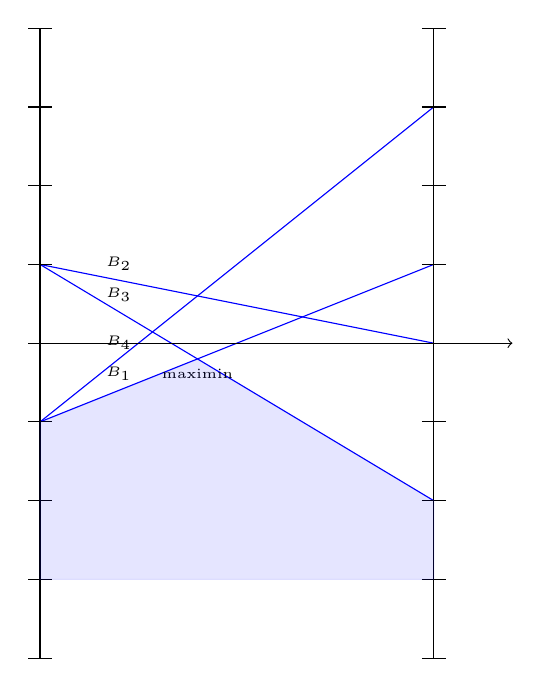
\begin{tikzpicture}[place/.style={circle,fill=violet}]
          \coordinate (a1) at (0,-1);
          \coordinate (b1) at (5,1);
          \coordinate (a2) at (0,1); 
          \coordinate (b2) at (5,0); 
          \coordinate (a3) at (0,1); 
          \coordinate (b3) at (5,-2); 
          \coordinate (a4) at (0,-1); 
          \coordinate (b4) at (5,3); 
          \coordinate (o) at (0,0); 
          \coordinate (p) at (5,0); 
          \coordinate (i) at (10/5,-1/5); 
          \draw[-, color=blue] (a1) -- (b1) node[pos=0.2, above, color=black] {\tiny $B_1$};;
          \draw[-, color=blue] (a2) -- (b2) node[pos=0.2, above, color=black] {\tiny $B_2$};;
          \draw[-, color=blue] (a3) -- (b3) node[pos=0.2, above, color=black] {\tiny $B_3$};
          \draw[-, color=blue] (a4) -- (b4) node[pos=0.2, above, color=black] {\tiny $B_4$};;
          \node (n1) at (i) [below] {\tiny maximin};
          \draw[->, color=black]  (o) -- (6,0); 
          \draw[-, color=black]  (o) -- (0,4); 
          \draw[-, color=black]  (p) -- (5,4); 
          \draw[-, color=black]  (o) -- (0,-4); 
          \draw[-, color=black]  (p) -- (5,-4); 
          \foreach \y in {-4,...,4}
          {
          \draw[-] (-0.15,\y) -- (0.15,\y);
          \draw[-] (4.85,\y) -- (5.15,\y);
          }
          \filldraw[color=blue, opacity=0.1] (a1) -- (i) -- (b3) -- (5,-3) -- (0,-3) -- (a1);
        \end{tikzpicture}
      }
    \end{figure}
  \end{center}
The maximin is the intersection of the lines $B_1$ and $B_3$, and the probabilities are obtained for the reduced $2\times 2$ table,
\begin{center}
  \begin{tabular}{|l|l|l|l|l|}
    \hline
          & $B_1$ & $B_3$ \\
    \hline
    $A_1$ & 1     & -2    \\ 
    $A_2$ & -1    & 1     \\ 
    \hline
  \end{tabular}
\end{center}

for which $\left(x_1, x_2\right) = \left(\frac{2}{5},\frac{3}{5}\right)$ and $\left(y_1,y_2\right) = \left(\frac{3}{5},\frac{2}{5}\right)$ and the value of the game is $\nu = -\frac{1}{5}$

\subsubsection*{Problem 2}
Solve the game graphically:

\begin{center}
  \begin{tabular}{|l|l|l|}
    \hline
    & $B_1$ & $B_2$ \\
    \hline
    $A_1$ & 2     & -3    \\
    $A_2$ & -1    & 2     \\
    $A_3$ & 1     & 1     \\
    $A_4$ & 3     & 0     \\
    \hline 
  \end{tabular}
\end{center}


In this case, player A will choose a strategy which will maximize the A's payoff, but B will try to choose a strategy that will minimize A's payoff. Hence, the lowest point of intersection of the lines from the top will be the value of the game.

\begin{center}
  \begin{tabular}{|l|l|}
    \hline
    \textbf{A's pure strategy} & \textbf{Expected payoff for A}       \\
    \hline
    $A_1$                      & $2y_1-3\left(1-y_1\right)=5y_1-3$    \\
    $A_2$                      & $-y_1+2\left(1-y_1\right) = -3y_1+2$ \\
    $A_3$                      & $1$                                  \\
    $A_4$                      & $3 y_1$                              \\
    \hline
  \end{tabular}
\end{center}


\begin{center}
    \begin{figure}[H]
      \centering \scalebox{0.8}{
        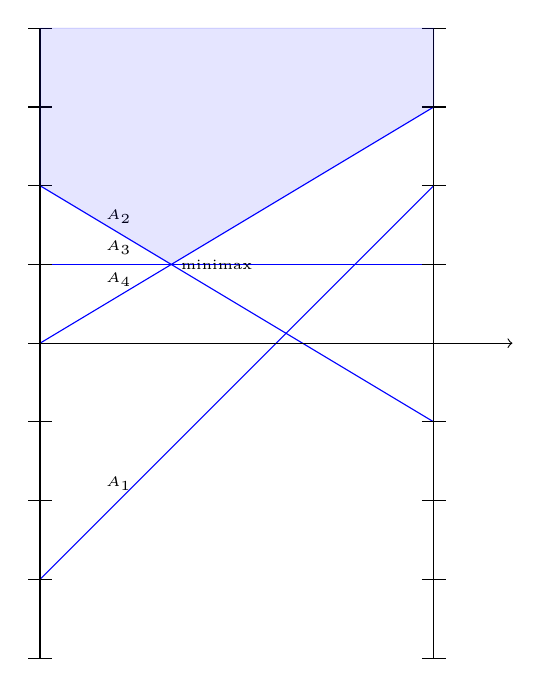
\begin{tikzpicture}[place/.style={circle,fill=violet}]
          \coordinate (a1) at (0,-3);
          \coordinate (b1) at (5,2);
          \coordinate (a2) at (0,2); 
          \coordinate (b2) at (5,-1); 
          \coordinate (a3) at (0,1); 
          \coordinate (b3) at (5,1); 
          \coordinate (a4) at (0,0); 
          \coordinate (b4) at (5,3); 
          \coordinate (o) at (0,0); 
          \coordinate (p) at (5,0); 
          \coordinate (i) at (5/3,1); 
          \draw[-, color=blue] (a1) -- (b1) node[pos=0.2, above, color=black] {\tiny $A_1$};;
          \draw[-, color=blue] (a2) -- (b2) node[pos=0.2, above, color=black] {\tiny $A_2$};;
          \draw[-, color=blue] (a3) -- (b3) node[pos=0.2, above, color=black] {\tiny $A_3$};
          \draw[-, color=blue] (a4) -- (b4) node[pos=0.2, above, color=black] {\tiny $A_4$};;
          \node (n1) at (i) [right] {\tiny minimax};
          \draw[->, color=black]  (o) -- (6,0); 
          \draw[-, color=black]  (o) -- (0,4); 
          \draw[-, color=black]  (p) -- (5,4); 
          \draw[-, color=black]  (o) -- (0,-4); 
          \draw[-, color=black]  (p) -- (5,-4); 
          \foreach \y in {-4,...,4}
          {
          \draw[-] (-0.15,\y) -- (0.15,\y);
          \draw[-] (4.85,\y) -- (5.15,\y);
          }
          \filldraw[color=blue, opacity=0.1] (0,4) -- (a2) -- (i) -- (b4) -- (5,4) -- (0,4); 
        \end{tikzpicture}
      }
    \end{figure}
  \end{center}
The lowest point from the top part of the graph is called the minimax point. 
The lines intersecting at the point are $A_2$ and $A_4$. So, we write the reduced table.

\begin{center}
  \begin{tabular}{|l|l|l|} \hline
          & $B_1$ & $B_2$ \\
    \hline
    $A_2$ & -1    & 2     \\
    $A_4$ & 3     & 0     \\
    \hline 
  \end{tabular}
\end{center}
Now, continue with finding the solution for mixed strategy. 

We find that $\left(x_1, x_2\right) = \left( \frac{1}{2}, \frac{1}{2}\right)$ and $\left(y_1,y_2\right) = \left(\frac{1}{3}, \frac{2}{3}\right)$ and the value of the game is $\nu = 1$

\subsubsection{Solving Games as a LPP}
Any game with a $m\times n$ payoff table can be solved as a linear programming problem in the following manner:

For Player A, the optimal mixed strategy can be solved using simplex method on the LPP

Maximize $x_{m+1}$

Subject to 
\begin{align*}
  p_{11} x_1 + p_{21} x_2 + \cdots +p_{m1} x_m - x_{m+1} & \ge 0 \\
  p_{12} x_1 + p_{22} x_2 + \cdots +p_{m2} x_m - x_{m+1} & \ge 0 \\
  \vdots                                                         \\
  p_{1n} x_1 + p_{2n} x_2 + \cdots +p_{mn} x_m - x_{m+1} & \ge 0 \\
  x_1+x_2+\cdots+x_m                                  & = 1   \\
  x_i \ge 0 \tag{for $i=1,2,\ldots ,m$}
\end{align*}

For Player B, the optimal mixed strategy can be solved using simplex method on the LPP

Minimize $y_{n+1}$

Subject to 
\begin{align*}
  p_{11} y_1 + p_{12} y_2 + \cdots +p_{1n} y_n - y_{n+1} &\le 0 \\
  p_{21} y_1 + p_{22} y_2 + \cdots +p_{2n} y_n - y_{n+1} &\le 0 \\
  \vdots \\
  p_{m1} y_1 + p_{m2} y_2 + \cdots +p_{mn} y_n - y_{n+1} &\le 0 \\
  y_1+y_2+\cdots+y_n                                  &= 1 \\
  y_i                                                &\ge 0 \tag{for $i=1,2,\ldots ,n$}
\end{align*}

For the previous problem, the LPP for player A can be written as:

Maximize  $x_5$

subject to
\begin{align*}
  2x_1-x_2+x_3+3 x_4-x_5 &\ge 0 \\
  -3x_1+2x_2+x_3-x_5     &\ge 0 \\
  x_1+x_2+x_3+x_4        &= 1 \\
  x_1,x_2,x_3,x_4        &\ge 0
\end{align*}

and for player B, the optimal probabilities can be found using the following LPP:

Minimize   $y_3$

subject to
\begin{align*}
  2y_1-3y_2     &\le 0 \\
  -y_1+2y_2-y_3 &\le 0 \\
  y_1+y_2-y_3   &\le 0 \\
  3y_1-y_3      &\le 0 \\
  y_1+y_2       &= 1 \\
  y_1,y_2       &\ge 0
\end{align*}
\end{document}

